\section{Grundlagen und Beugung}
\subsection{TITAN Elektronenmikroskop}
Das in diesem Teil verwendete Mikroskop ist das FEI TITAN 80-300, welches im Laufe von 3 Laboreinheiten für unterschiedlichen Problemstellung verwendet wurde.

Das FEI TITAN 80-300 ist ein hoch auflösendes Transmission Elektronenmikroskop, welches zusätzlich für die off Axis Holographie ausgerüstet wurde. Das Mikroskop hat eine 80-300 kV Schottky Field Emission Electron Gun mit der eine Ortsauflösung von ca. 80 pm erreicht werden kann.

\begin{figure}[htbp]
 \centering
 \includegraphics[width=0.7\textwidth]{Grundlagen&Beugung/TITAN_Mikroskop.jpg}
 \caption[FEI TITAN 80-300]{Bild des FEI TITAN 80-300, mit off Axis Holographie ausgerüstet }
 \label{TITANMikroskop}
\end{figure}


\subsection{Transmissionselektronenmikroskopie}

Die Transmissionselektronenmikroskopie ist ein Abbildungsverfahren bei der mit Hilfe eines Elektrons strahl ermöglicht wird.\\
Bei diesem Verfahren wird eine dünne Probe mit dem Elektronenstrahl durchleuchtet, die Beschleunigung Spannungen für den Elektronenstrahl befinden sich im Bereich von 80 bis 400 kV.\\
Beim Durchdringen der Probe werden Elektronen elastisch und inelastisch gestreut, mit Hilfe von Adäquaten Objektiv und Pojektivlinsen können dieser fokussiert werden und durch eine Phosphor Leuchtschirm oder einem Szintillation-CCD System sichtbar gemacht werden.

\subsection{Mikroskop check und Alignement}
Um das Mikroskop in Betrieb zu nehmen müssen einige Checks und Ausrichtungen vorgenommen werden. Diese können wie in folgenden zusammengefast werden: Vakuum Check, Elektronenstrahl Finden, Kondensor einstellen, Astigmatismus korrigieren, Pivotpunkte korrigieren, Rotationszentrum Einstellen und Zemlin Tableaus.

\subsubsection{Vakuum Check}
Es muss überprüft werden ob der Druck in im Mikroskop und den einzelten Kammern unter Bestimmten Werten liegt, ("Octagon" <25 log). Fall dies nicht der Fall ist und die „Column valves“ geöffnet werden kann das zum Schaden an der Elektronen Gun und Sensoren kommen. Wenn der druck ausreichend niedrig ist und Gase nicht weiter ausgepumpt werden müssen können die „Column valves“ (Vakuum Schleusen) geöffnet werden.\\
Zum Abpumpen stehen dem Mikroskop Turbopumpen und  Ionenpumpen zur Verfügung.

\subsubsection{Elektronenstrahl Finden}
Falls nach dem Öffnen der Vakuumschleuse der Elektronenstrahl nicht auf dem Leuchtschirm zu sehen ist muss dieser zuerst gefunden werden. Dafür ist es von Vorteil die Vergrößerung herunter zu fahren, dann kann die Probe Verfahren werden so dass der Elektronenstrahl hindurch fallen kann. Zudem muss der Strahl mit Hilfe des „Beam Shift“ auf die Mitte des Leuchtschirm verfahren werden.

\subsubsection{Kondensor einstellen}
Der Kondensor muss anschließend eingestellt werden, dafür werden folgende Einstellungen verwendet:
\begin{itemize}
  \item Gun lens 1
  \item Spot size 1
  \item C2 ~34%
  \item C2 Blende (100um)
\end{itemize}
Die C2 Blende zentriert: Um eine Blende zu benutzen wird zuerst mit der „Intensity“ der Elektronenstrahl auf den ganzen Leuchtschirm ausgeweitet. Dann wird eine blende in den Strahlengang eingefahren, diese Blende liegt vor der zweiten Kondensor Linse.  Der Schatten der Blende kann nun mit Hilfe der Multifunktion Knöpfe in die Mitte des Leuchtschirmes gefahren werden.

\subsubsection{Einstellung der Probenhöhe}
Um die probenhöhe nach dem Einsetzen eine neue Probe zu ermitteln, muss man einigen Schritten folgen.\\
Im Mikroskop ist ein Standardfokus festgelegt, der Euzentrische Fokus. Damit nicht bei jeder Probe der Euzentrische Fokus neu festgelegt werden muss wird versucht die Probe in diesen Ebene zu verfahren. Dabei wird die Probe entlang der Optischen Achse verfahren. Danach wird ein Stück amorphes Material in der Probe gesucht und identifiziert, durch Proben verfahren (X,Y Richtung) und der Kondensor Linse C2 wird dann dieser Bereich ausgeleuchtet. Im Imaging Modus wird dann der stahl zusammengezogen und auf einen kleinen Punkt fokussiert, dabei entstehen um den Leuchtpunkt Beugungsringe. Die Probe kann nun Endlage der Optischen ebene verfahren werden bis sich die Ringe in den Nullstrahl auf einen Leuchtfleck zusammenziehen.  An diesem Punkt ist die Probe grob am der Brennebene angekommen.\\
Wenn der Elektronenstrahl (Intensity) wieder aufgezogen wird sollte die Probe recht gut fokussiert sein. Wenn die Probe nun an einen Punkt verfahren wird an dem Probenmaterial und Vakuum sichtbar ist, kann durch leichter Justierung des Fokus kann das Bild so eingestellt werden das der Kontrast zwischen Vakuum und Probenmaterial am geringsten ist oder gar verschwindet, an diesem Punkt ist der beste Fokus erreicht. \\
Anschließend kann durch verstellen des Fokus in den Unter-/Oberfokus gewechselt werden. Hierbei wird dann der Kontrast zwischen Vakuum und Probe stärker.

\subsubsection{Astigmatismus des Kondensorsystem korrigieren}
Der Astigmatismus entsteht, wenn der Elektronenstahl mehrere Brennlinien hat. Bei der Mikroskopie ist das durch Zwei Fokusse zu erkennen, bei den jeweiligen Fokussen ist nur eine Ebene fokussierst so das in der senkrecht dazu stehenden Achse ein Unter-/Überfokus entsteht und/oder die Objekte auf dem Leuchtschirm gestreckt wirkt. Um diesen Fehler zu korrigieren, wird ein Quadrupol Stigmator verwendet, dieser kann durch variieren die Brennpunkte auf dieselbe ebene führen und eine gute Fokussierung herbeiführen. Wenn der Elektronenstrahl durch die C2 Linse zusammengezogen wird, bildet dieser dann einen symmetrischen Punkt auf dem Leuchtschirm ab, wenn ein oval entsteht ist das ein Indiz auf einen Astigmatismus.

\subsubsection{Entkopplung von Strahlkippung und -Verschiebung}
Im Elektronenmikroskop kann der Elektronenstrahl durch mehrerer Ablenkspulen verkippt werden. Dabei wird der Strahl um bestimmten Punkt verkippt, dieser ist der sogenannte Pivotpunkt. Dieser Punkt kann für die x und y Richtung des Strahls unterschiedlich sein und müssen so eingestellt werden das die am gleichen Ort liegen. Wenn der Pivotpunkt richtig eingestellt ist wird der Fokus beim verkippen des Strahles nicht beeinflusst.

\subsubsection{Grobe Korrektur der Koma}
Wenn das rotationszentrum der Elektronenstrahl nicht richtig eingestellt ist, verändern sich die Größen und Position der auf dem Leuchtschirm zu erkennenden Strukturen. Mit Hilfe der Multifuntions Knöpfe kann das rotationszentrum so eingestellt werden das die Strukturen beim Rotieren unverändert bleiben.

\subsubsection{Zemlin Tableau}
Um die übrig gebliebenen Bildfehler zu korrigieren wird mit der Software und der CCD Camara ein Zemlin Tableau erstellt. Mit Hilfe einer Fast Fourier Transformation kann dann die Bildfehler identifiziert und in den korrigiert wenden. Die Bildfehler die korrigiert werden sind die z.B. Sphärische Aberration, Defokus, Axialecoma und two-/three-fold Astigmatismus.\\
Dies ist ein meist repetitiver Prozess, die Korrekturen sind auch zeitlich limitiert da sich die Einstellungen im Mikroskop durch thermische Effekte schnell verändern


\subsection{Aufnehme im Fokus Über-/Unterfokus}

Um sich mit dem Mikroskop besser vertraut zu machen wurden einige TEM Aufnahmen erstellt.\\
Hierfür wurde eine Standardprobe verwende diese bestand aus einem Kohlenstoff film auf dem Latex Kugeln und Goldpartikeln aufgebracht waren.\\
Zuerst wurden eine Reihe von Bildern aufgenommen um den Fokus, Unter- und Überfokus zu veranschaulichen, siehe \cref{TEMStandardprobe}.


\begin{figure}
     \centering
     \begin{subfigure}[b]{0.3\textwidth}
         \centering
         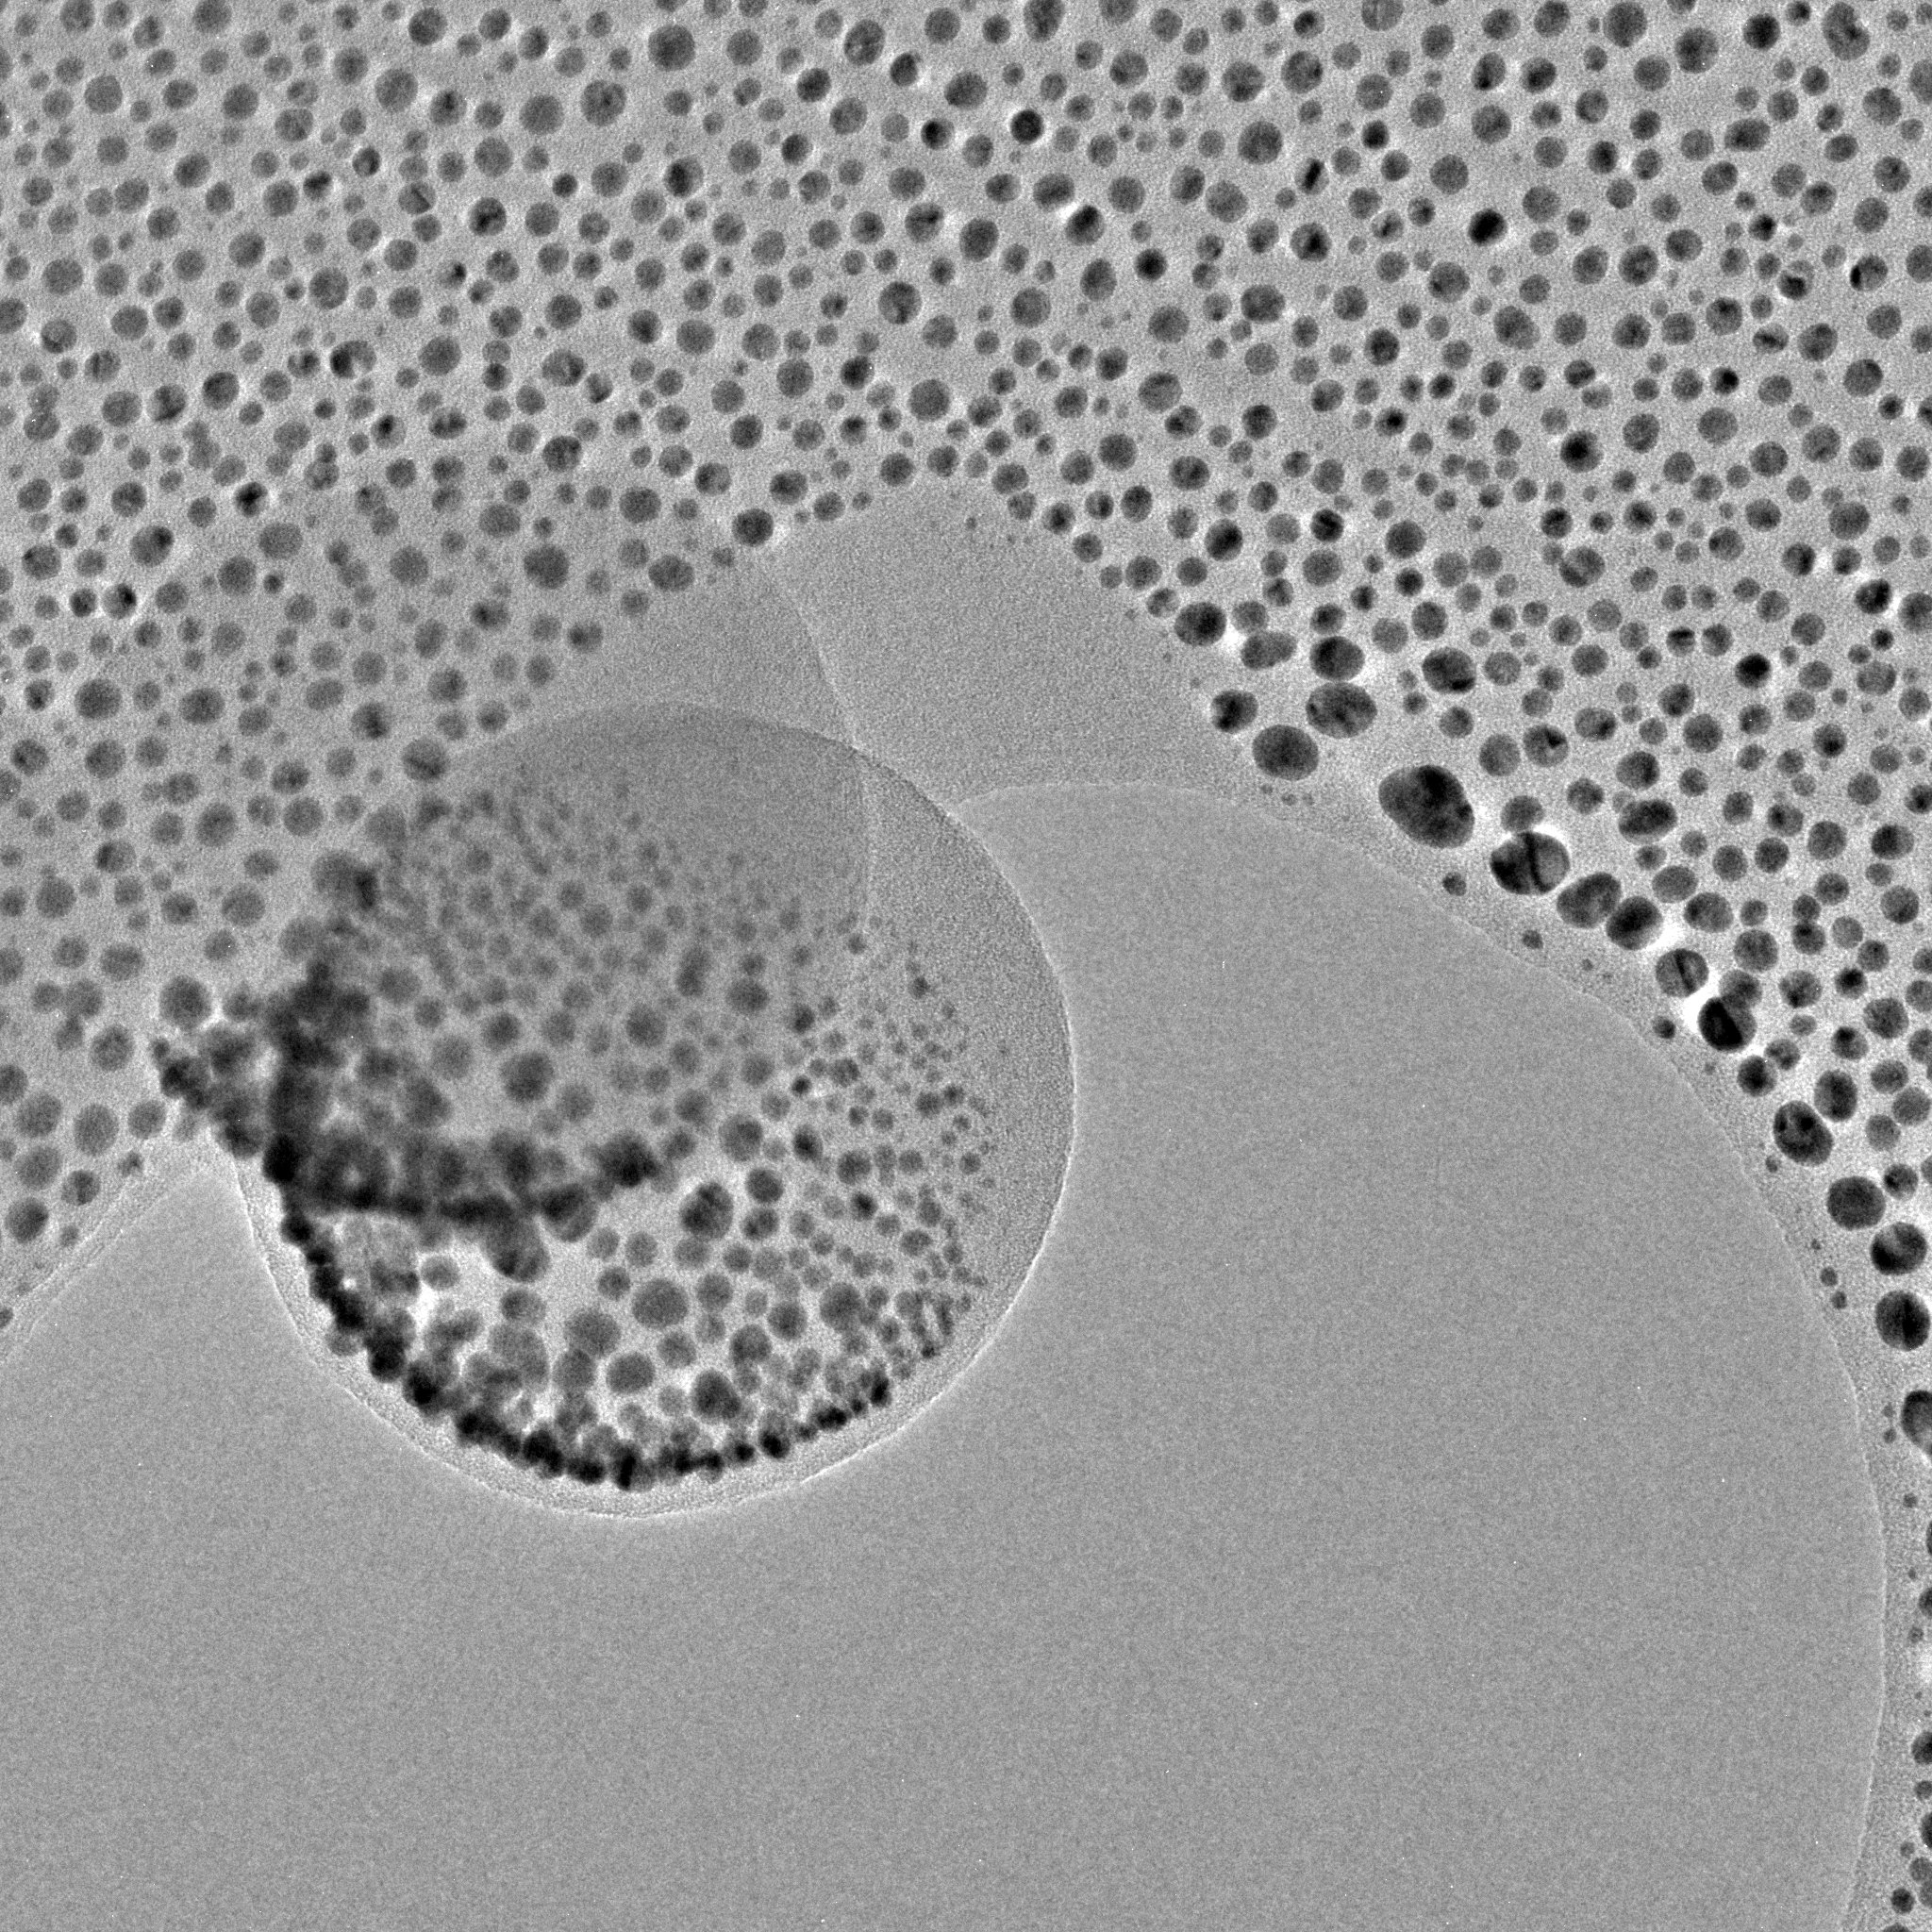
\includegraphics[width=\textwidth]{Grundlagen&Beugung/Lateckugel_Im_Fokus.jpg}
         \caption{Im Fokus}
         \label{SPFokus}
     \end{subfigure}
     \hfill
     \begin{subfigure}[b]{0.3\textwidth}
         \centering
         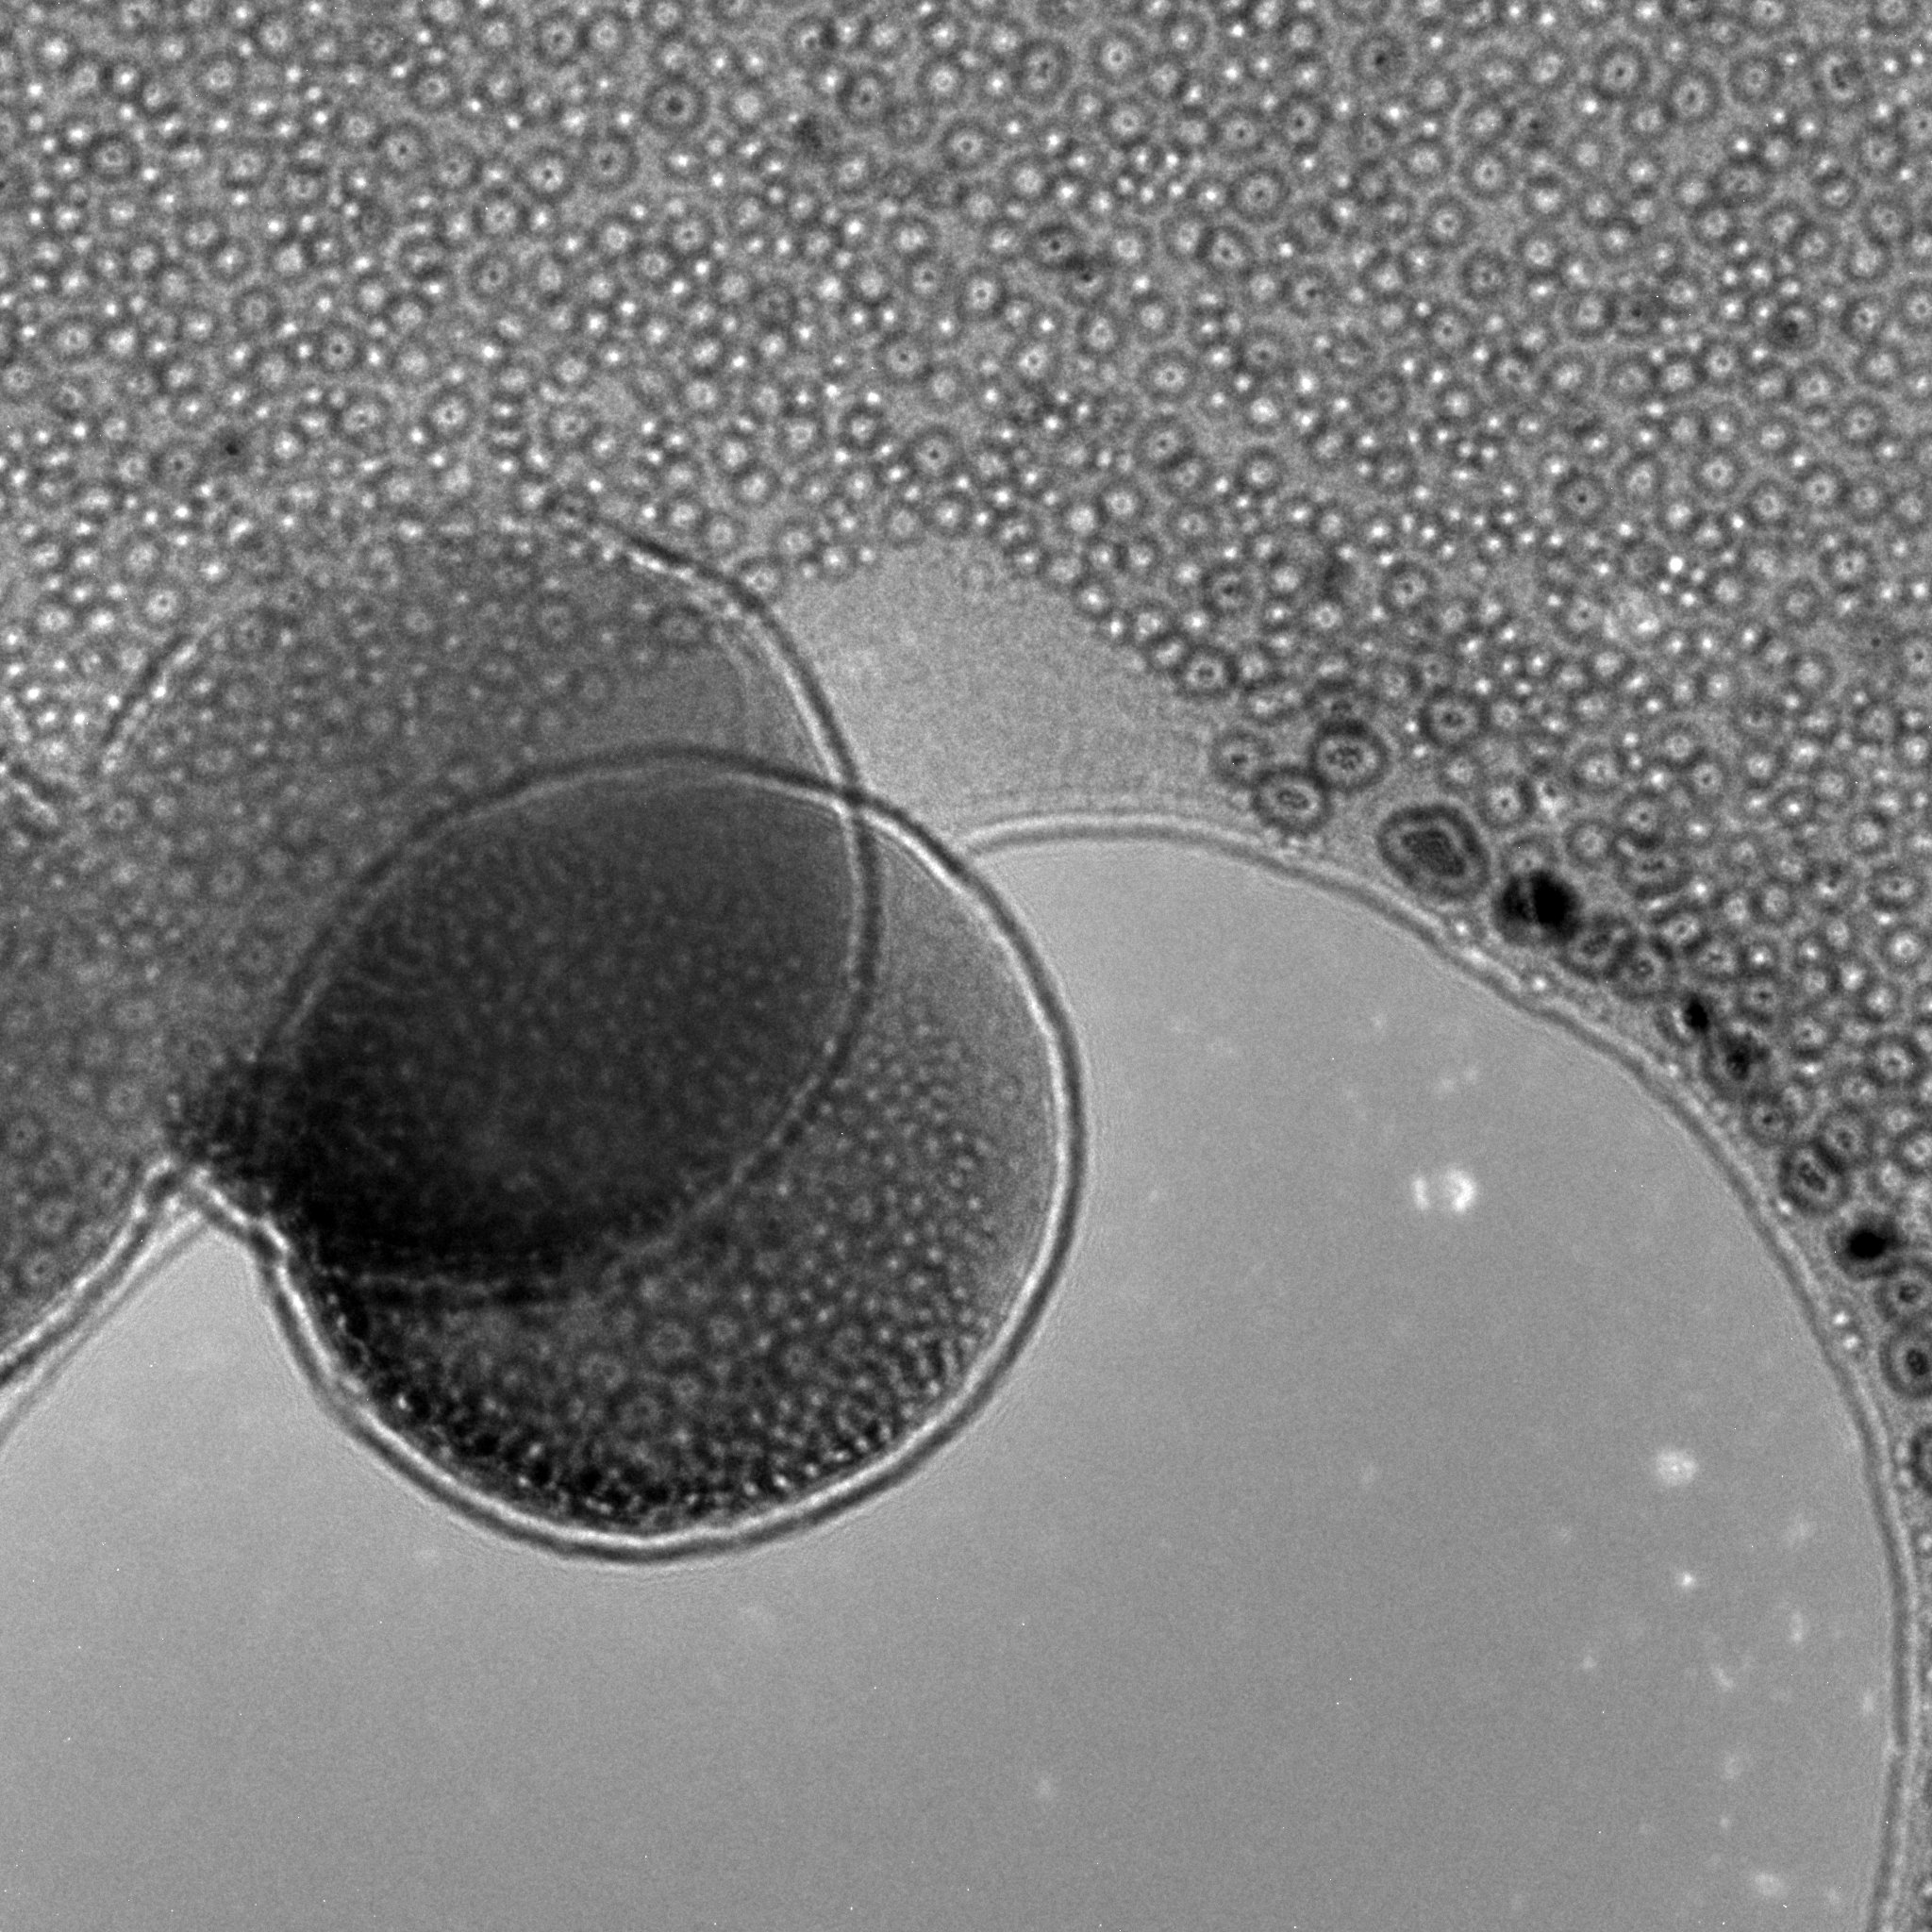
\includegraphics[width=\textwidth]{Grundlagen&Beugung/Latexkugeln_Im_Überfokus.jpg}
         \caption{Überfoku}
         \label{SPÜberfoku}
     \end{subfigure}
     \hfill
     \begin{subfigure}[b]{0.3\textwidth}
         \centering
         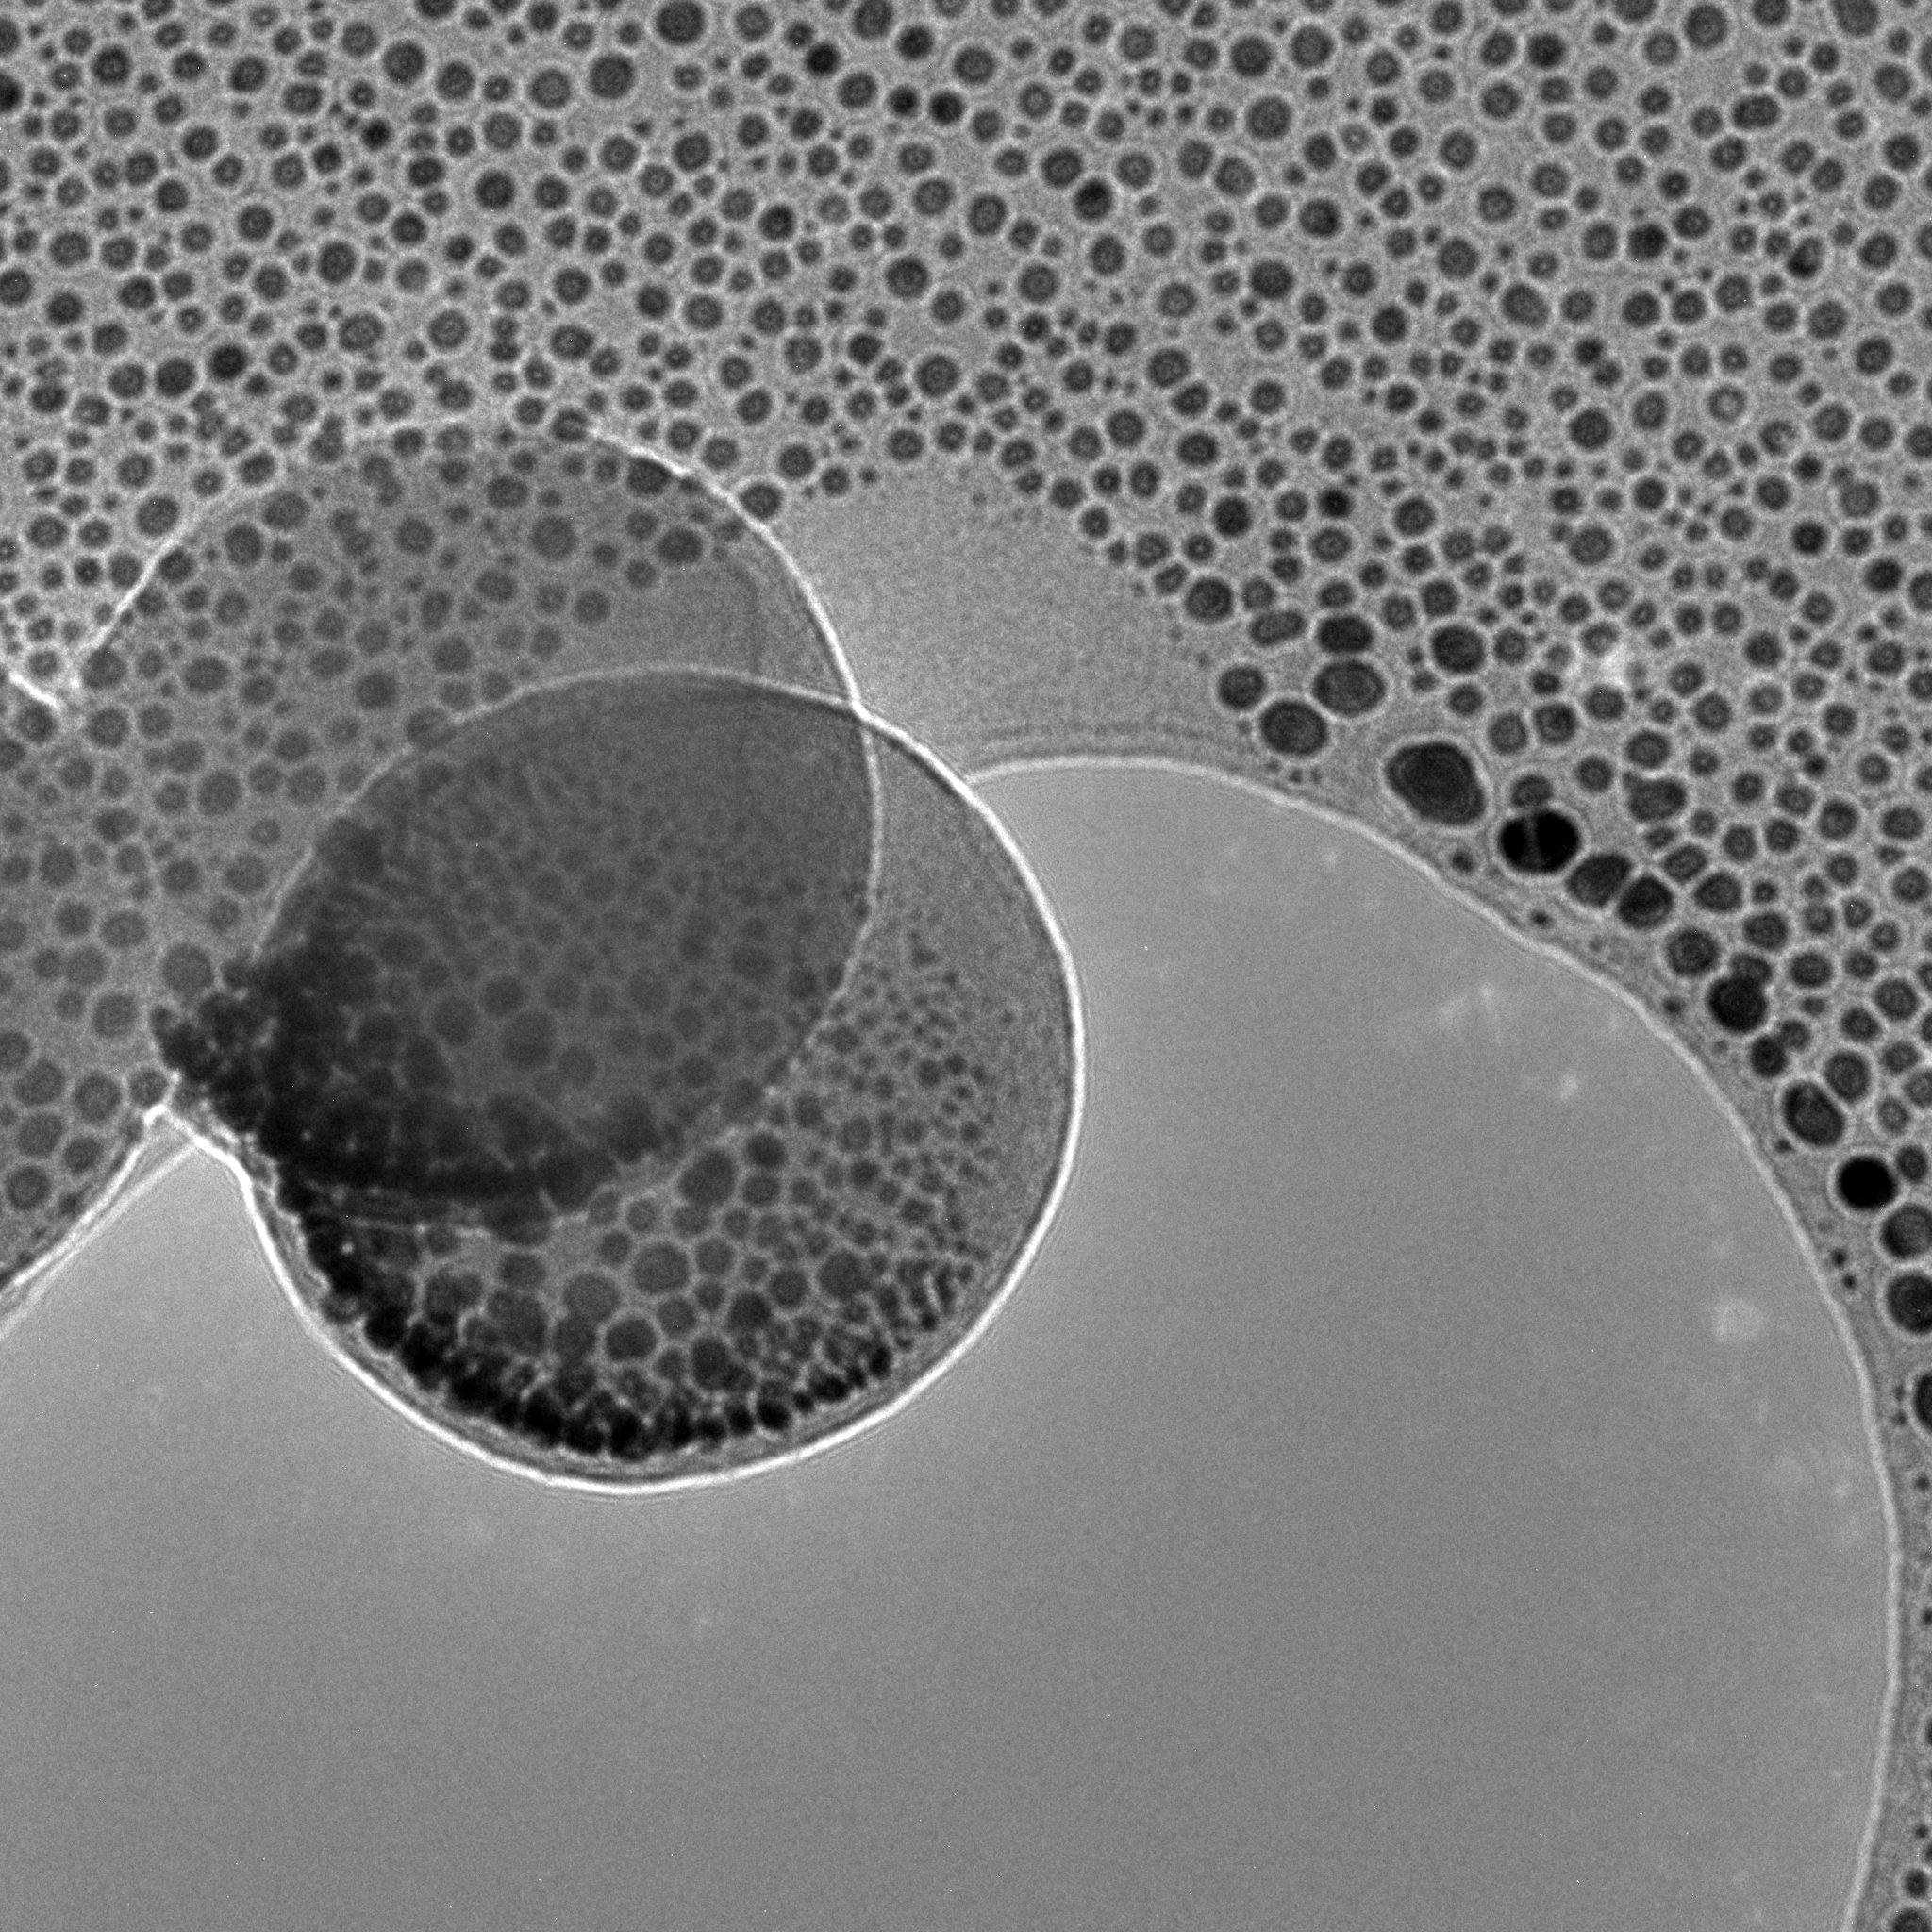
\includegraphics[width=\textwidth]{Grundlagen&Beugung/Latexkugeln_Im_Unterfokus.jpg}
         \caption{Unterfokus}
         \label{SPUnterfokus}
     \end{subfigure}
        \caption{TEM Aufnahmen eine Standardprobe, mit Kohlenstofffilm, Latex Kugeln und Goldpartikeln}
        \label{TEMStandardprobe}
\end{figure}

Am Bild im Fokus sind einige Elemente der Probe gut erkennbar: Es ist ein Kohlenstoff Film zu erkennen, dieser Film weist ein Loch an der Unteren kante der Aufnahme auf in dieser Region ist nur Vakuum abgebildet. Es sind außerdem die vergleichsweise großen Latex Kugeln und die kleineren Goldpartikel auf die auf dem Kohlenstoff Film aufgebracht sind Erkennbar. Hier wird der starke Kontrast zwischen den schweren Gold Partikeln und dem leichten Kohlestoff und Latex gut sichtbar. Der Kontrast zwischen Kohlestoff Film und Vakuum ist hingegen sehr schwach was auf einen guten Fokus hindeutet.\\
Der Überfokus entsteht, wenn die Probe entlang der optischen Achse leicht vor der Objektebene der Objektlinse positionirt ist. Bei der Aufnahme des Überfokus ist ein starker dunkler Kontrast am Rand/Saum des Kohlefilms erkennbar. Der Kontrast zwischen den Goldpartikeln und dem Kohlenstoff ist dagegen geringer als zuvor. \\
Im Unterfokus ist die Probe etwas hinter der Objektebene der Objektlinse positioniert, dabei ist ein Weißer Rand am der Kohlenstofffilm Kante zu erkennen, der Kontrast zwischen den Latex kugeln, den Goldpartikeln und dem Kohlenstofffilm ist jedoch immer noch ziemlich gut. In diesem Modus ist es leichter unterschiedliche Strukturen in der Probe auseinander zu halten und zu identifizieren.\\
Der helle und der dunkle Fresnel-Saum bei den defokussierten Abbildungen ergibt sich durch Interferenzerscheinungen. Entstehen durch die Beugung der Elektronenwelle an der Kohlenstoffkante.

\subsubsection{Gold-Cluster}
Die Gold Partikel wurden mit dem HRTEM in einer höheren Vergrößerung genauer angeschaut. Mit dieser Einstellung ist eine atomare Auflösung möglich, und erste Kristallstruktur Strukturen erkennbar. In der Aufnahme \cref{TEMGoldcluster} sind mehrerer Cluster zu erkennen, und auch die Orientierung und Anordnung der Goldatome innerhalb der einzelnen Cluster ist erkennbar. Die Cluster heben sich gegen den amorphe kohlestofffilm gut ab.

\begin{figure}[htbp]
 \centering
 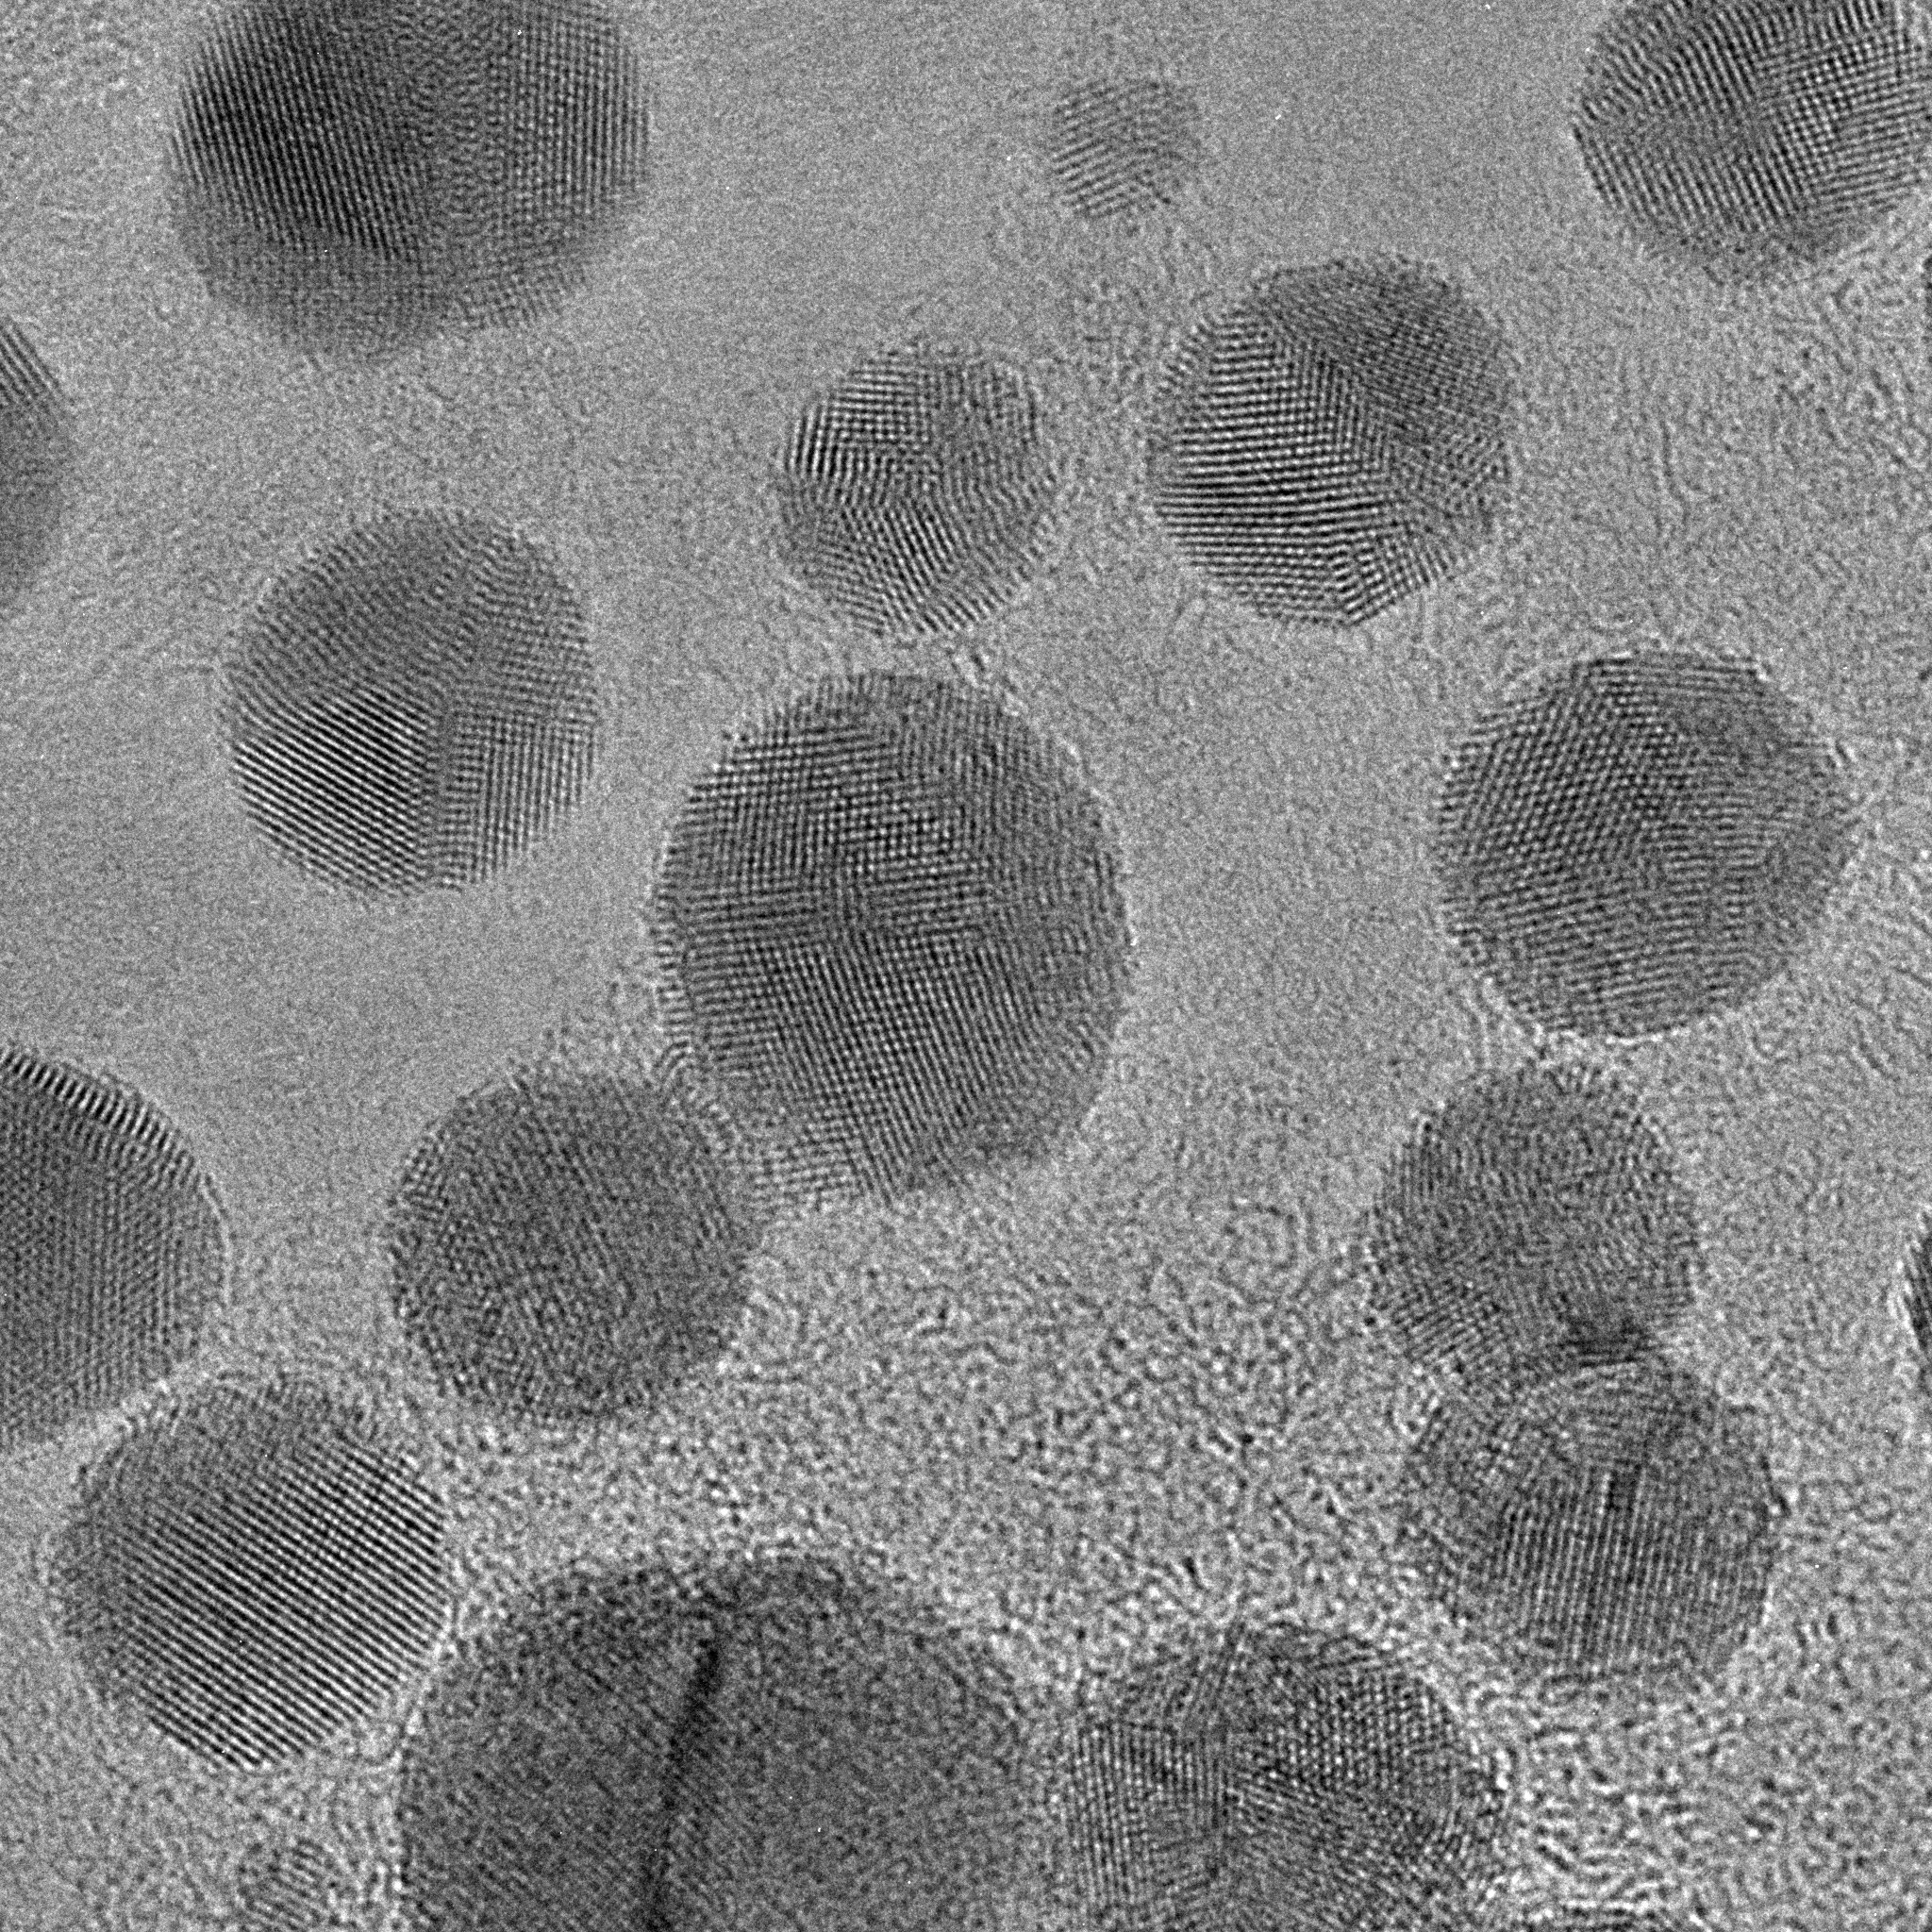
\includegraphics[width=0.7\textwidth]{Grundlagen&Beugung/Goldpartikel_im_leichten_ueberfokus.jpg}
 \caption[TEM Gold cluster]{TEM Aufnahme von Gold Cluster auf Kohlestofffilm}
 \label{TEMGoldcluster}
\end{figure}

\subsection{Aufnehmen von Beugungsbildern}
Um ein Beugungsbild aufzunehmen muss zuerst im Bildmodus des Mikroskops eine adäquate stelle auf der Probe identifiziert werden und die ins Zentrum des Leuchtschirmes verfahren werden. Um ins Beugungsbild zu wechseln muss der „Diffraction“ Knopf am Steuer Panel gedruckt werden. Dies Verändert die Leistung der „Diffraction lense“ (DL) und „Projection lense“ (PL) linsen so dass ein Beugungsbild abgebildet wird. Um die CCD Kamera vor zu starker Einstrahlung zu schützen muss vor dem hochklappen des Leuchtschirm ein „Beam Stopper“ in den null strahl verfahren werden. Zusätzlich können SA Blende eingebracht werden, in diesen versuch wurde eine 10 Mikrometer und 40 Mikrometer Blende verwendet. Das Beugungsbild kann nun nach dem hochklappen des Leuchtschirm und ausfahren der CCD Kamera aufgenommen werden.

\subsubsection{Beugungsbilder der Au Probe mit verschiedenen Blenden}

Zuerst wurde ein Bild mit einem SA Blende von 10 Mikrometer aufgenommen, das Beugungsbild ist auf einem amorphen kohlenstofffilm Teil der Probe aufgenommen. Die Beleuchtungszeit der CCD Kamera betrug 8 Sekunden (siehe Abbildung \cref{AU10um} ).\\
Die dieser Blenden Größe sind vor allem vereinzelte Punkte zu erkennen, diese bilden auch schon Andeutungen von ringen. Beugungsringe entstehen bei einer polykristallinen Probe mit unterschiedlichen kristallographischen Orientierungen. Jedoch kann, wenn nur einige wenige Kristall Orientierungen beleuchtet werde, sich die beleuchtungsringe nicht vollständig schließen.

\begin{figure}[htbp]
 \centering
 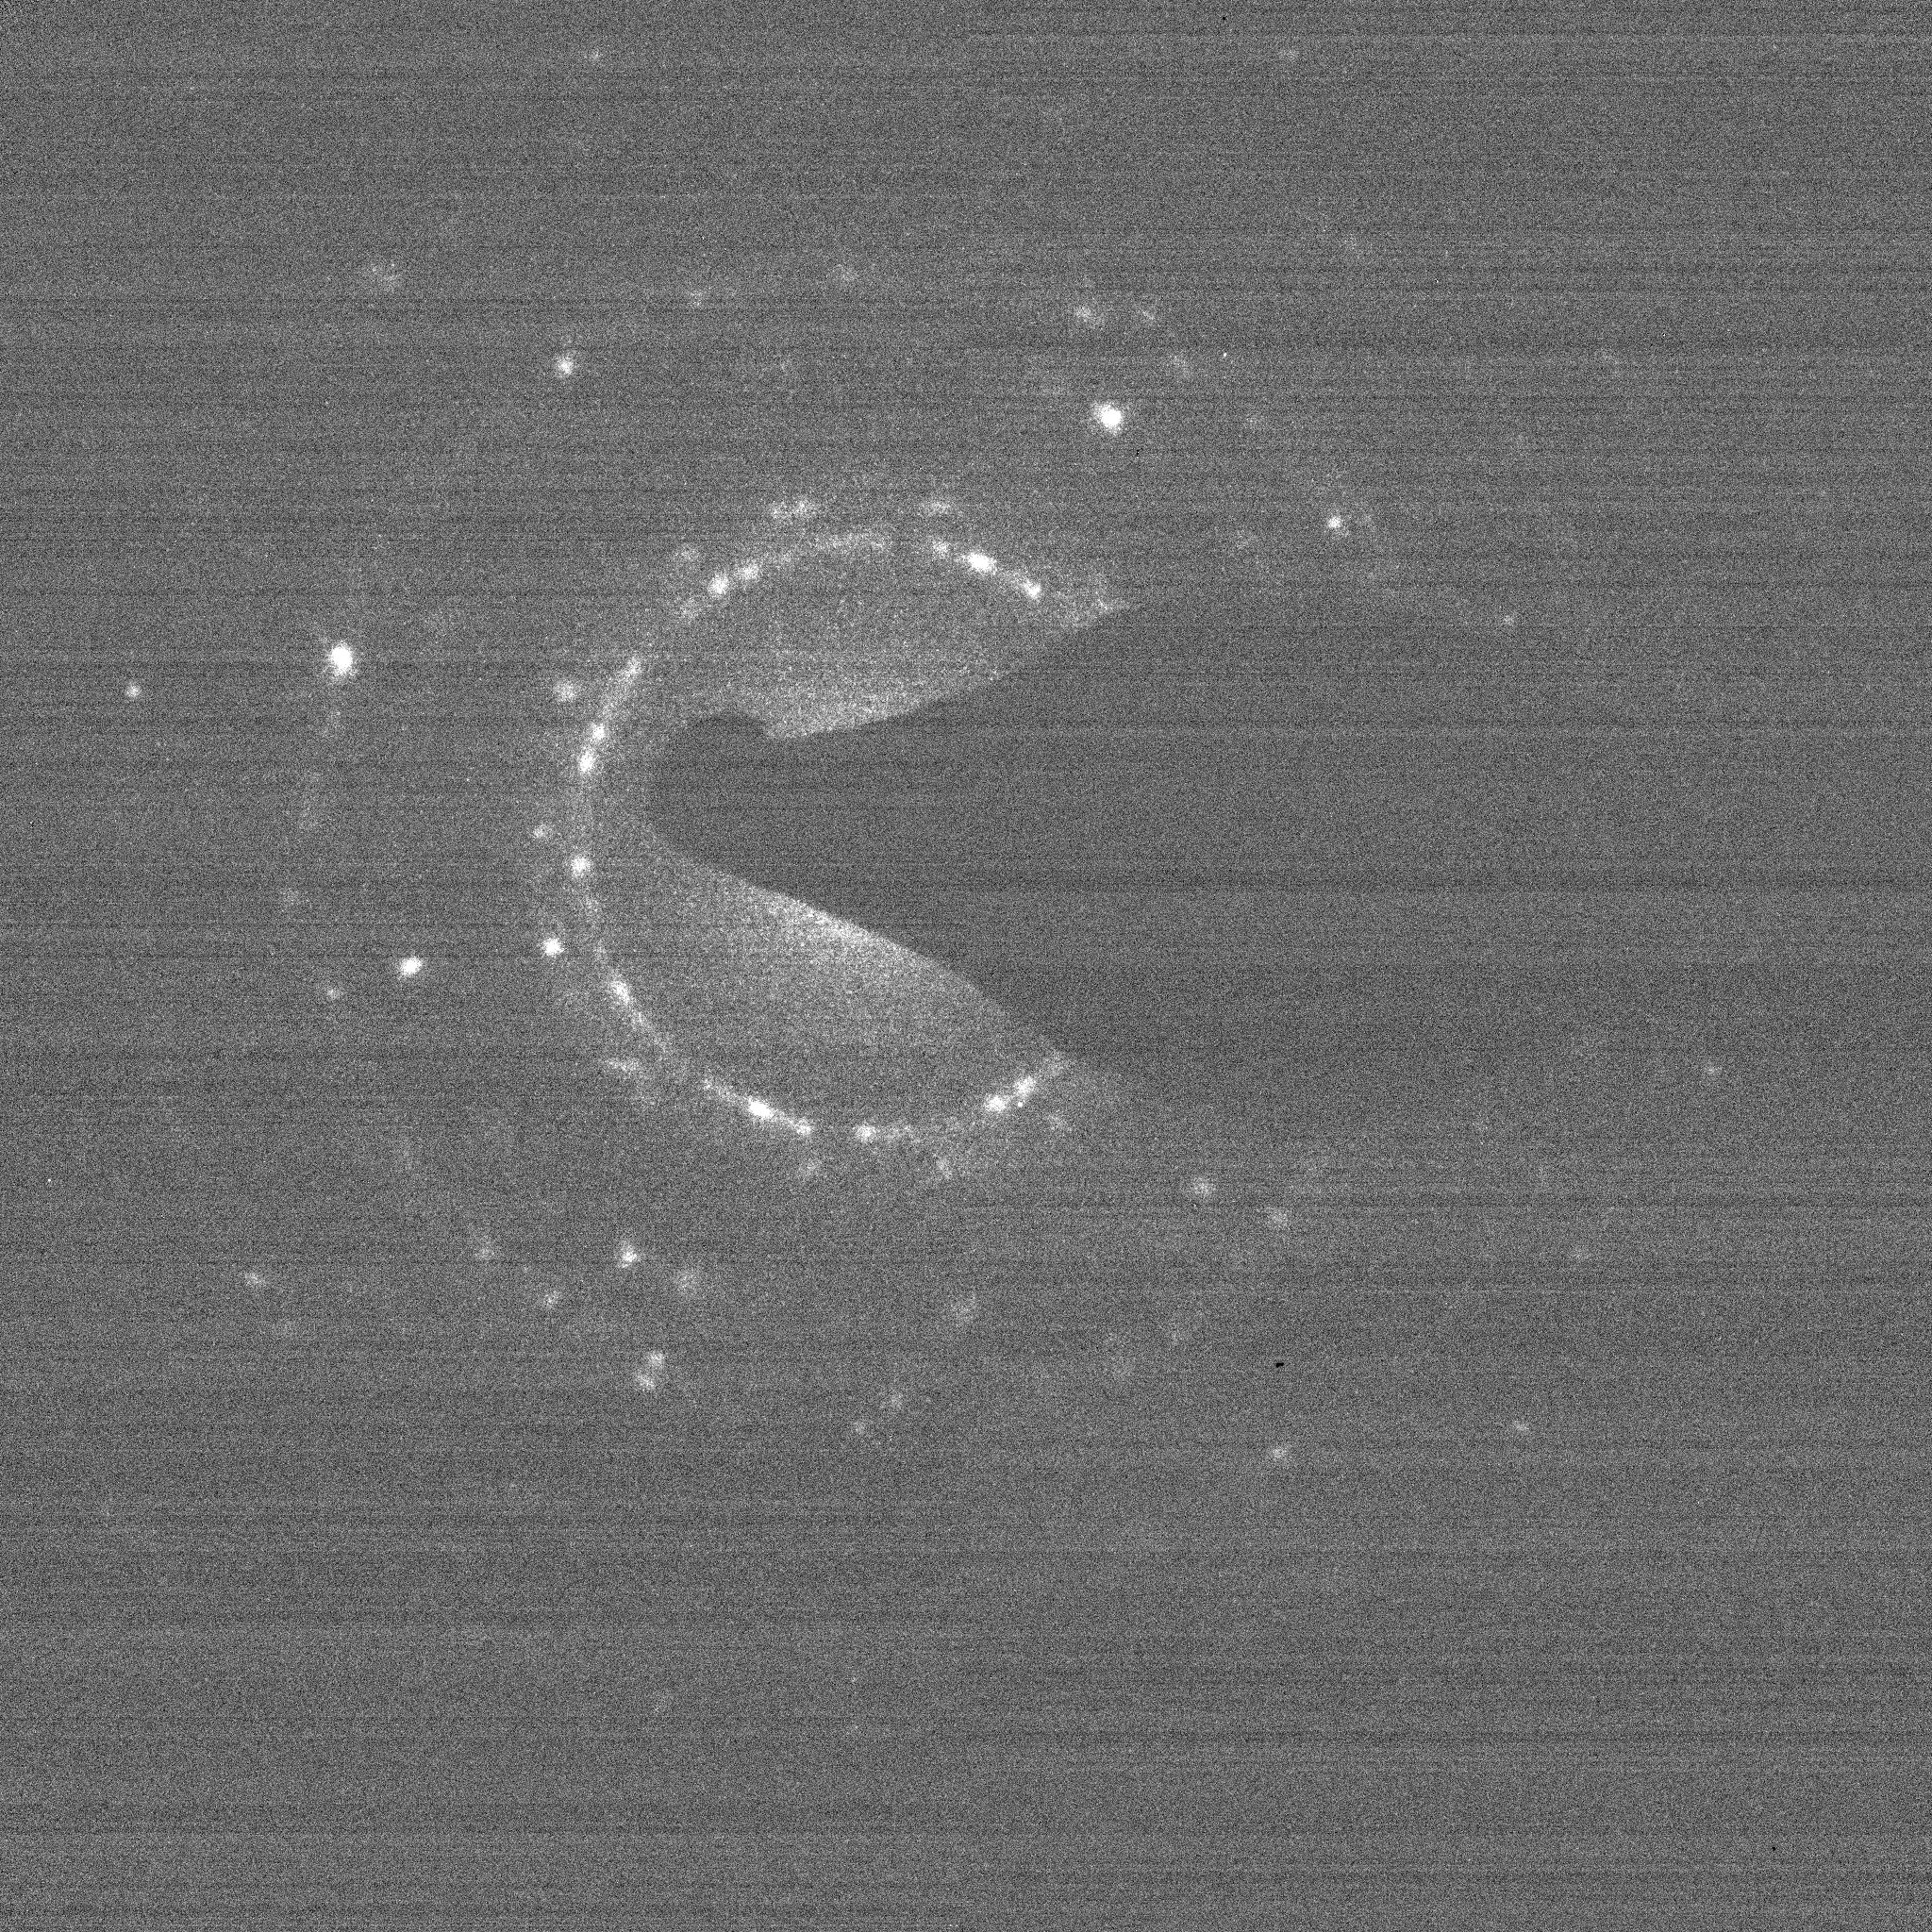
\includegraphics[width=0.7\textwidth]{Grundlagen&Beugung/Blende_10_Beugung_8sec.jpg}
 \caption[Beugungsbild Au 10µm Blede]{TEM Beugungsbild aufnahme von Au Cluster mit 10µm SA-Blende und 8 sec Beleuchtungszeit}
 \label{AU10um}
\end{figure}

Anschließend wurde ein Beugungsbild mit einer SA Blende von 40 Mikrometer aufgenommen. Die Beleuchtungszeit betrug 4 Sekunden (siehe Abbildung \cref{AU40um}). Hierbei sind die ringförmigen Muster abgebildet, einzelne Punkte sind dennoch gut erkennbar.

\begin{figure}[htbp]
 \centering
 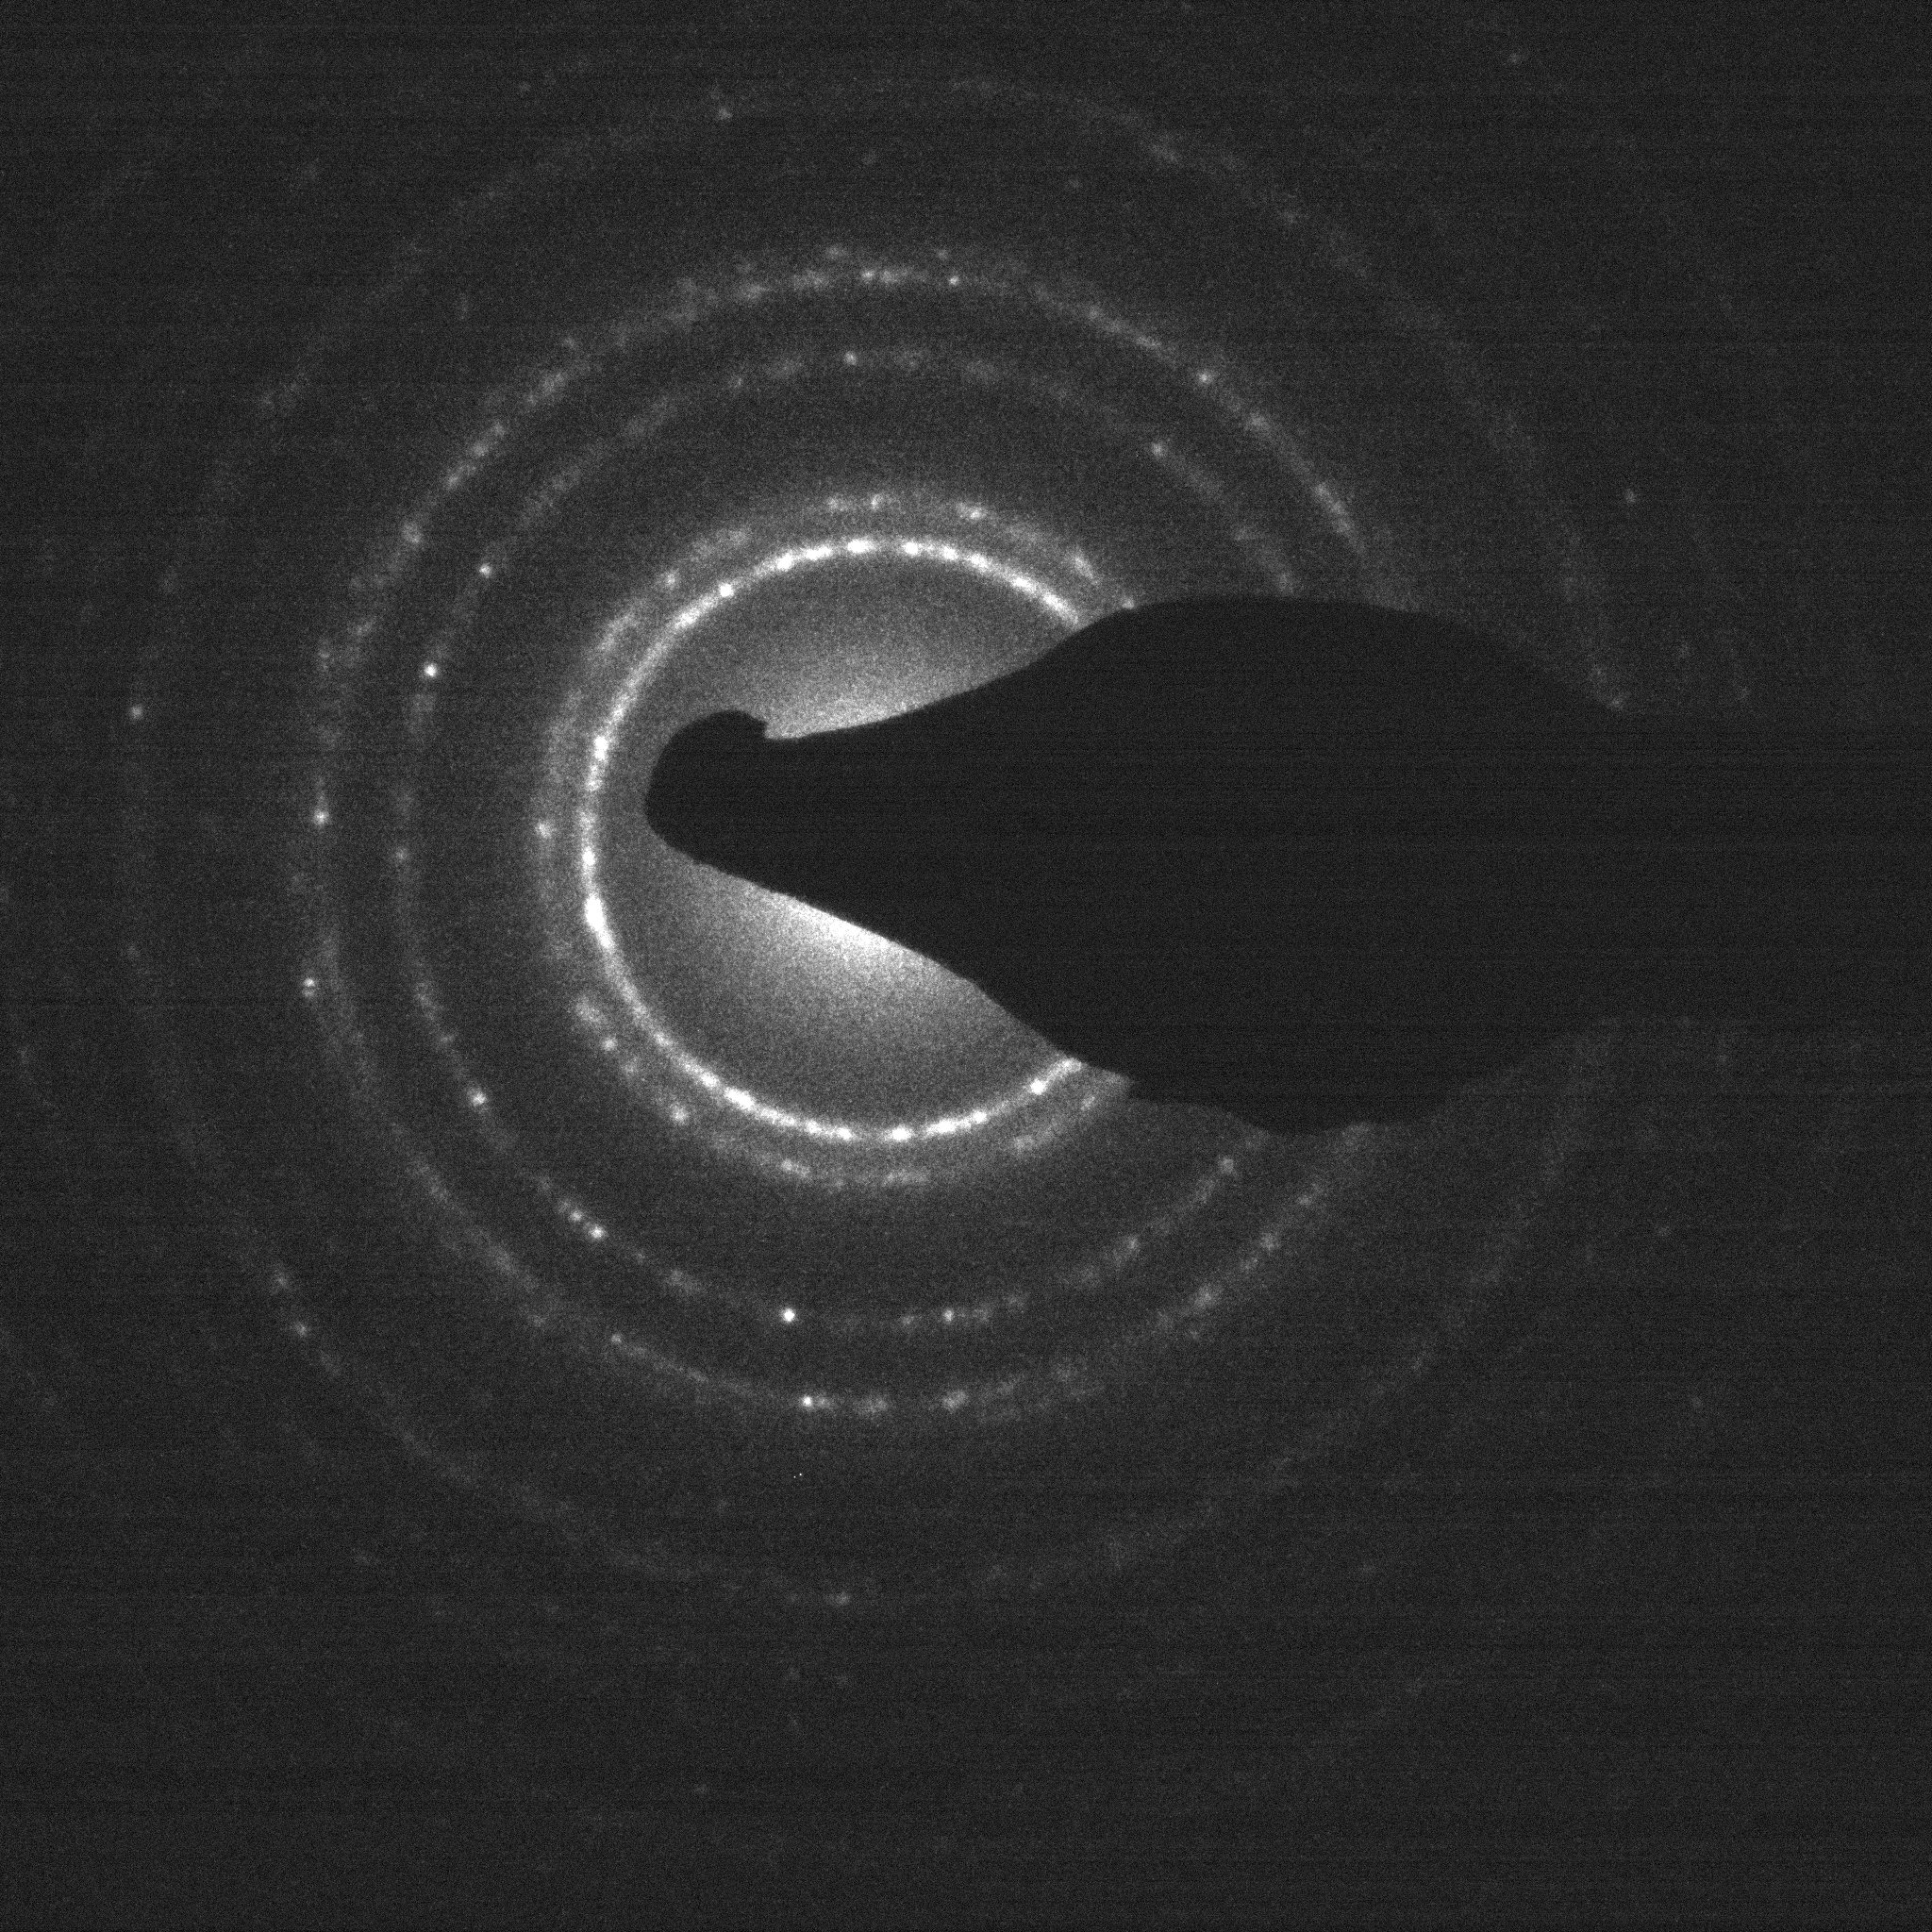
\includegraphics[width=0.7\textwidth]{Grundlagen&Beugung/Blende_40_Beugung_4sec.jpg}
 \caption[Beugungsbild Au 40µm Blede]{TEM Beugungsbild aufnahme von Au Cluster mit 40µm SA-Blende und 4 sec Beleuchtungszeit}
 \label{AU40um}
\end{figure}

\subsection{Hell-/ Dunkelfeld aufnehmen}
Die Standardprobe und insbesondere eine Latex Kugel wurde sich zusätzlich zum „Brightfield“, in dem vor allem die Streuabsorption der Probe abgebildet wird, auch das „Darkfield“ angeschaut. Beim Darkfield wird vor allem die Streuung an der Probe abgebildet.\\ 
Um ein Darkfield Aufnahme zu erlangen wird gibt es Zwei Möglichkeiten die im Laufe des Versuchs auch beide ausprobiert wurden. Das „dirty Dakfield“ und das „Centered Darkfield“.
\subsubsection{Dirtk darkfield}
Beim Dirty darkfield wird im Beugungsbild eine Beugungsblende vom Zentrum weg zu einem brechungsreflex verfahren. Wenn anschließend ins Bildmodus zurück gewechselt wird sind dann nur Elektronen aus diesem Brechungsreflex zu sehn. Es kann dann ein so genanntes Darkfield Bild aufgenommen werden. Hierbei kann es zu Bildfehlern kommen so das diese Methode nicht optimal ist.

\subsubsection{Centered Darkfield}
Bei Centered Darkfield, wird anstatt die Blende zu verfahren der Elektronenstrahl so verkippt das der gewünschte Reflex durch das Loch in der zentrierten Beugungsblende fällt. Dies hat denselben Effekt wie bei Dirty darkfild aber ohne die Bildfehler, und kann so einen Duknkelfeld Bild aufgenommen werden.

\subsubsection{Standard Probe Hell/Dunkel Feld Aufnahmen}
Bei der Hellfeld Aufnahme der Standard Probe sind die Goldpratikel recht gut durch ihren hohen dunklen Kontrast zu erkennen. Dies last sich durch den schweren Gold Atome erklären die eine Größe Streuung verursachen. Die Latex Kugeln sind ebenfalls gut erkennbar. Der Kohlenstofffilm zeigt jedoch nur einen sehr geringen Kontrast auf.\\
Bei der Centerd Darkfield Aufnahme sind vor allem die Goldpartikel mit einem Besonders guten Kontrast zu erkennen da sie sich Hell vom Dunklen Hintergrund abheben. Nicht alle Goldcluster sind jedoch gleichermaßen gut sichtbar. Dies wird durch die unterschiedliche Orientierung der Kristallstrukturen der jeweiligen Cluster zu erklären. Die Latex Kugeln sind auch in diesem Modus noch erkennbar. Der Kohlefilm hingegen ist quasi nicht sichtbar. 

\begin{figure}
     \centering
     \begin{subfigure}[b]{0.49\textwidth}
         \centering
         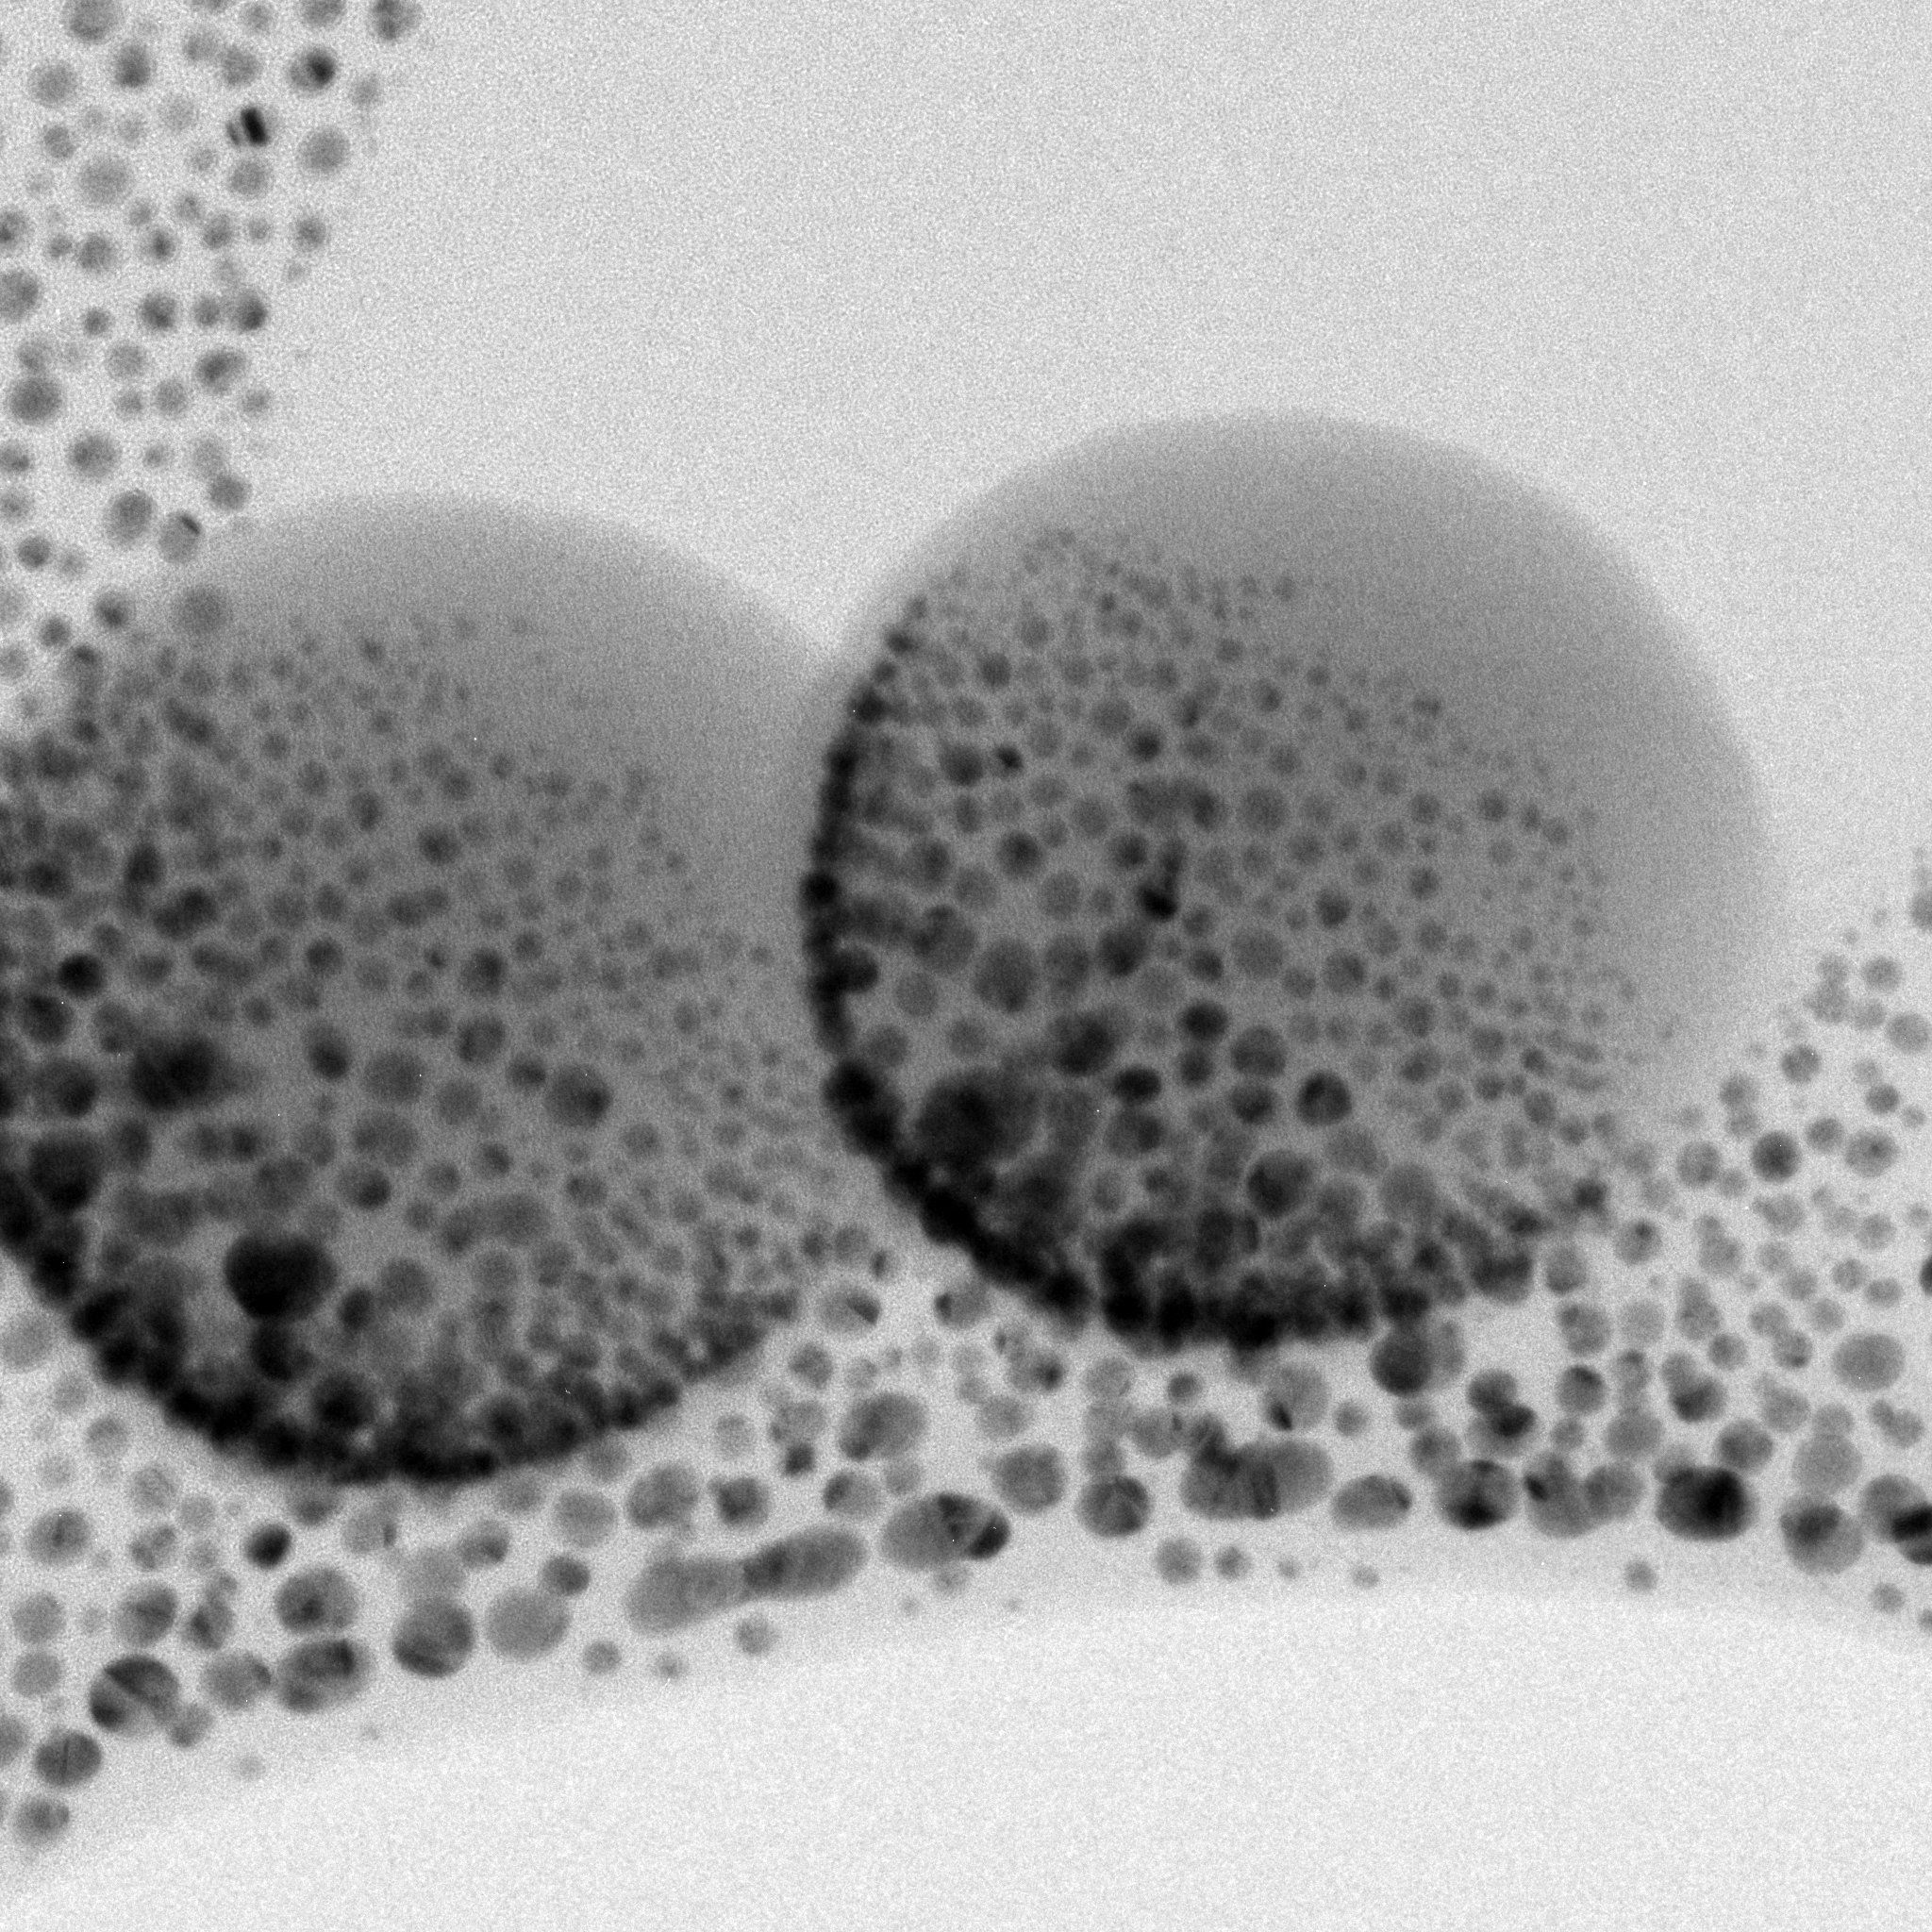
\includegraphics[width=\textwidth]{Grundlagen&Beugung/Goldpartukel_1sec_brightfeeld2.jpg}
         \caption{Brightfield}
         \label{SPBF}
     \end{subfigure}
     \hfill
     \begin{subfigure}[b]{0.49\textwidth}
         \centering
         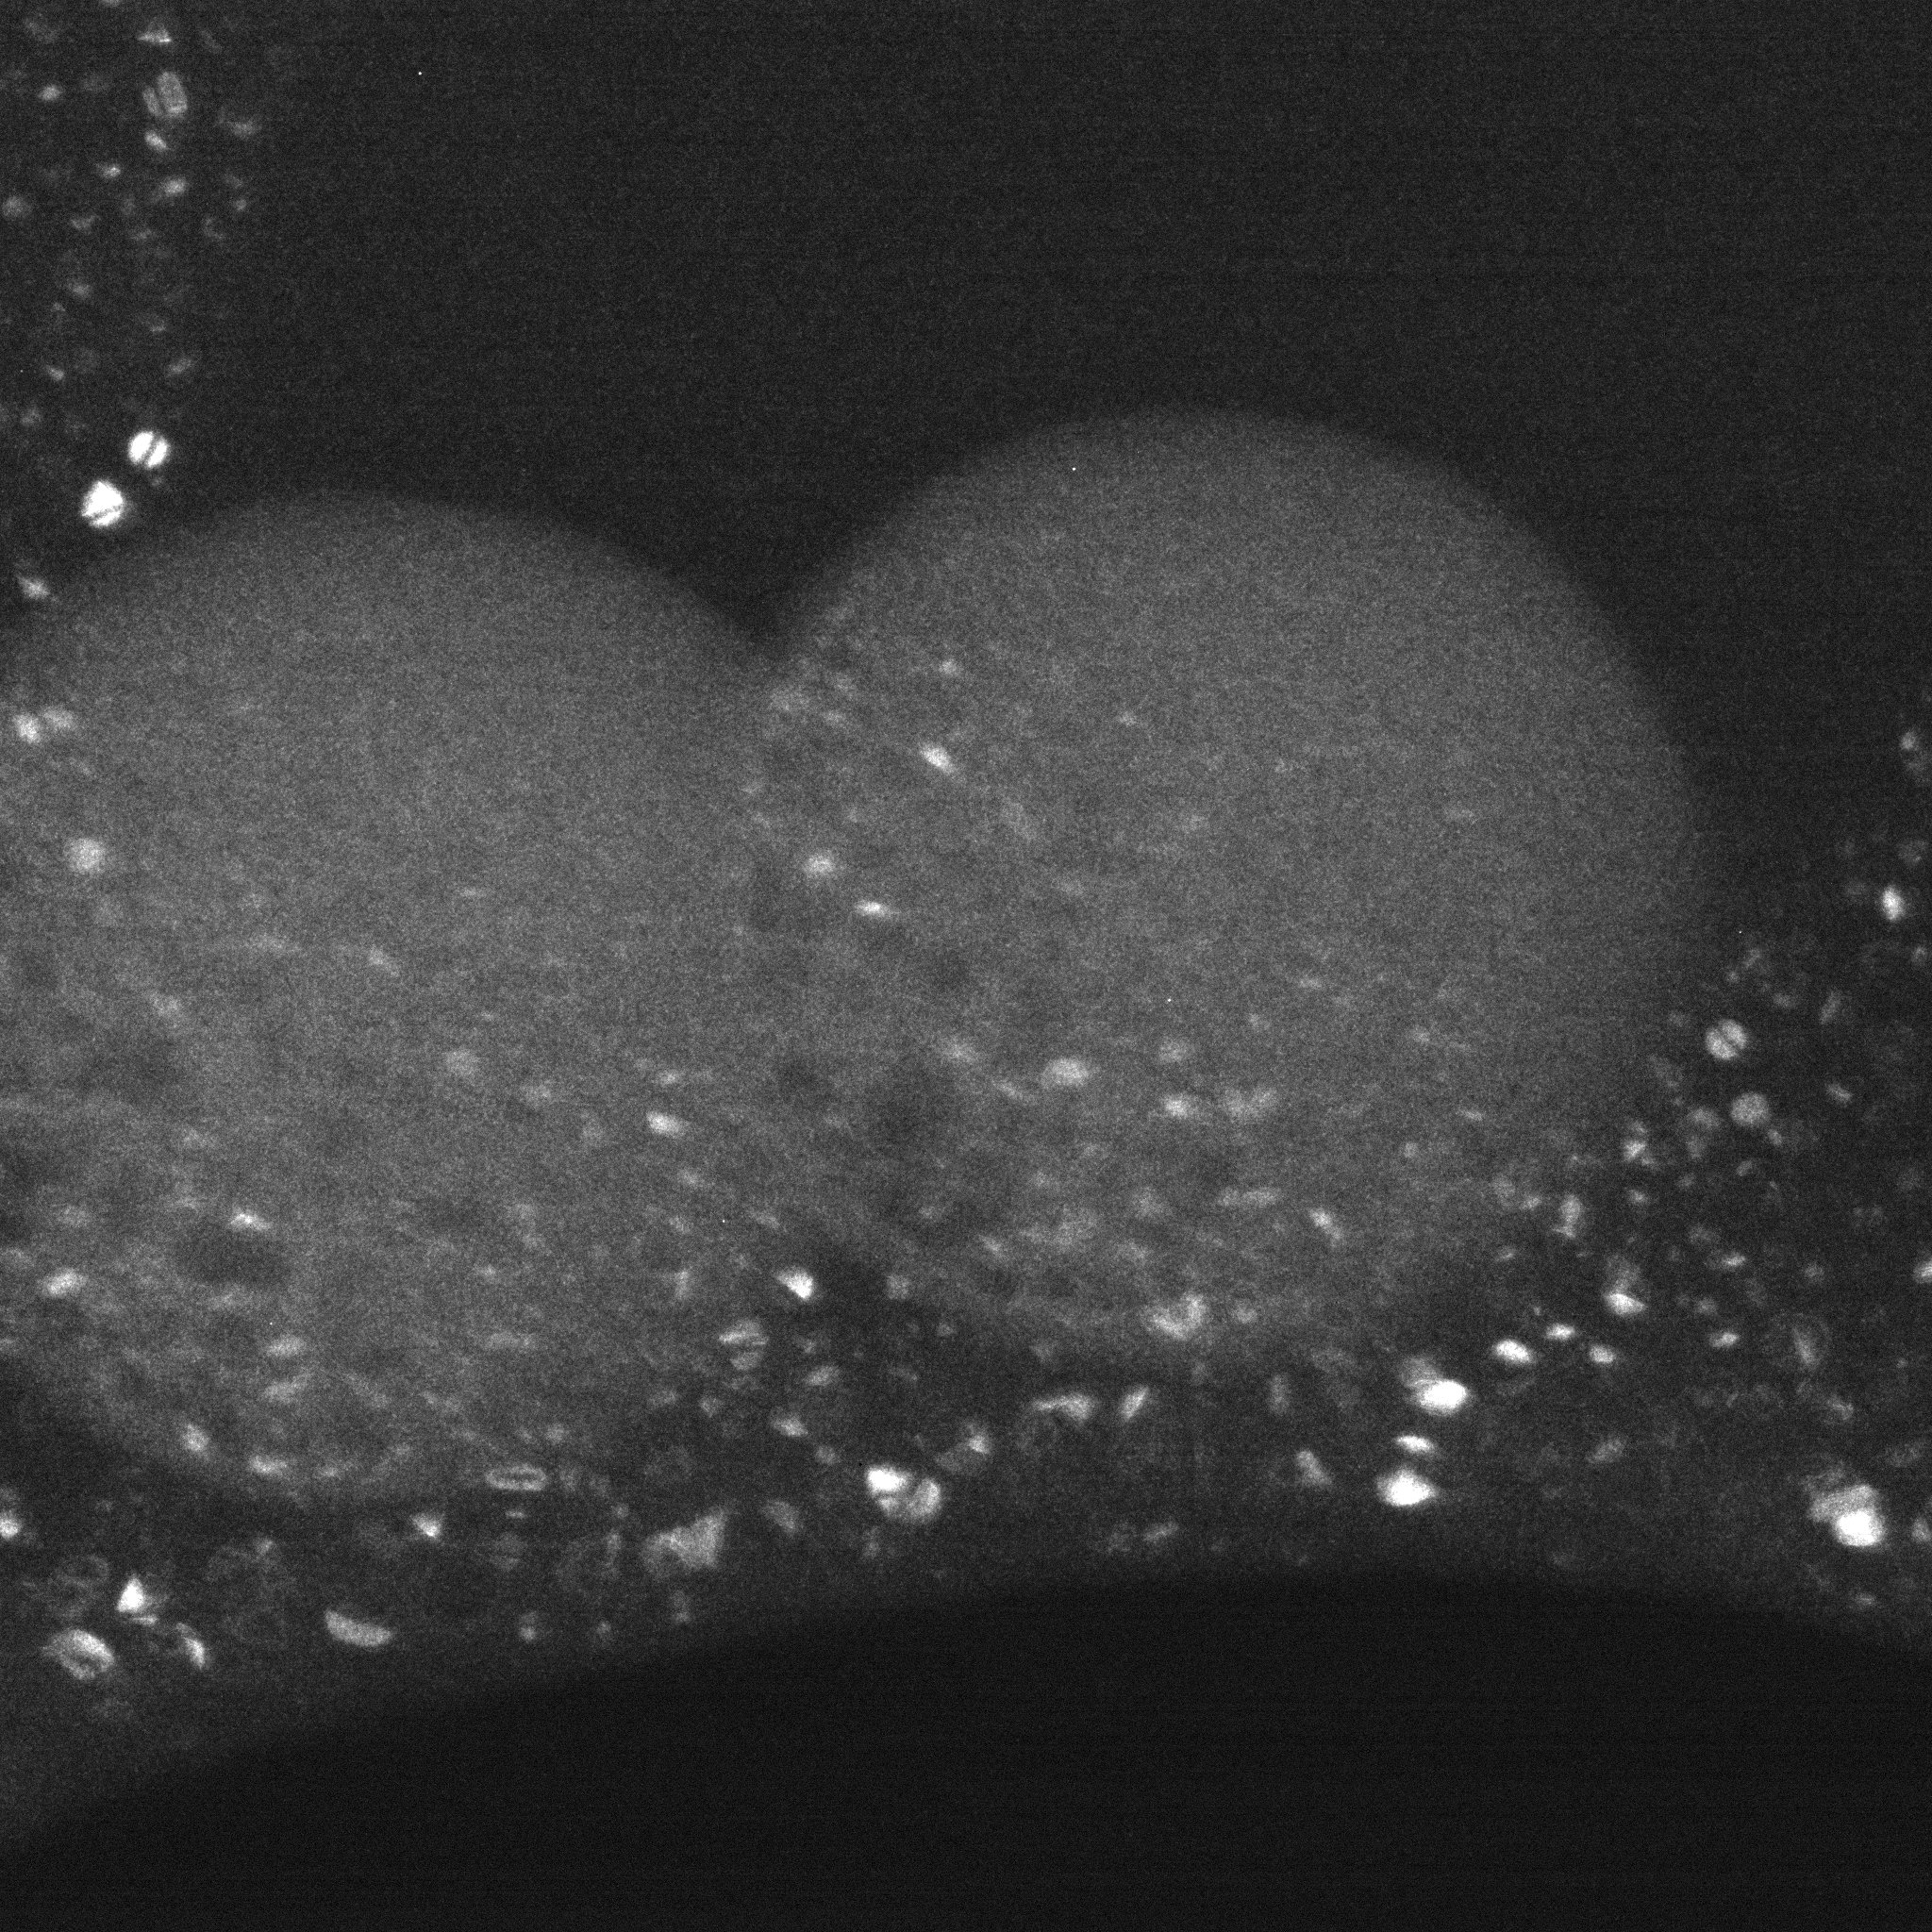
\includegraphics[width=\textwidth]{Grundlagen&Beugung/Goldpratikel_1sec_darkfeeld2_andererWinkel.jpg}
         \caption{Darkfield}
         \label{SPDF}
     \end{subfigure}
        \caption{Bright-/Centered Darkfield Aufnahme der Standard Probe (Kohlenstoff, Latex, Gold), 1 sec Beleuchtungszeit}
        \label{SPBF&DF}
\end{figure}

\subsection{InGaAs/GaAs Struktur}

Um die eigen angefertigt Probe aus der vorher beschriebenen Sektion „Probenpräperation“ genau zu untersuchen, mussten die Proben im Mikroskope getauscht werden. Dabei musste die das Schleusen und die Vakuum System wie zuvor aufgeführt bedient und gecheckt werden. Nach dem tauschen der Probe und einer Entlüftung und Stabilisierungszeit von ca. Einer Stunde musste das Mikroskope wieder neu eingereicht werden.  Dies wurde nach dem zuvor beschriebenen Schema durchgeführt.\\
An der eigenen Probe wurde zunächst versucht ein HRTEM Bild aufnehmen, Hierfür wurde ein geeignete dünne stelle an der Probe Identifiziert. Diese befand sich nahe der Klebesstelle an der Lochkante welches durch die Ionen Dünnung endstanden ist.\\
Nach dem Wechseln zum „Diffraction Mode“ konnte mithilfe der Beugungsbildes und den Kikuchi Linien die Probe so verkippt werden das TEM Aufnahmen entlang einer Zonenachse möglich war. Im Bild Modus wurde dann eine gute Aufnahme des Kristall Struktur mit atomarer Auflösung gemacht. Zudem wurden wieder Aufnahmen im unter-/Über Fokus erstellt. (Siehe Abbildung \cref{EigeneProbe}).

\begin{figure}
     \centering
     \begin{subfigure}[b]{0.49\textwidth}
         \centering
         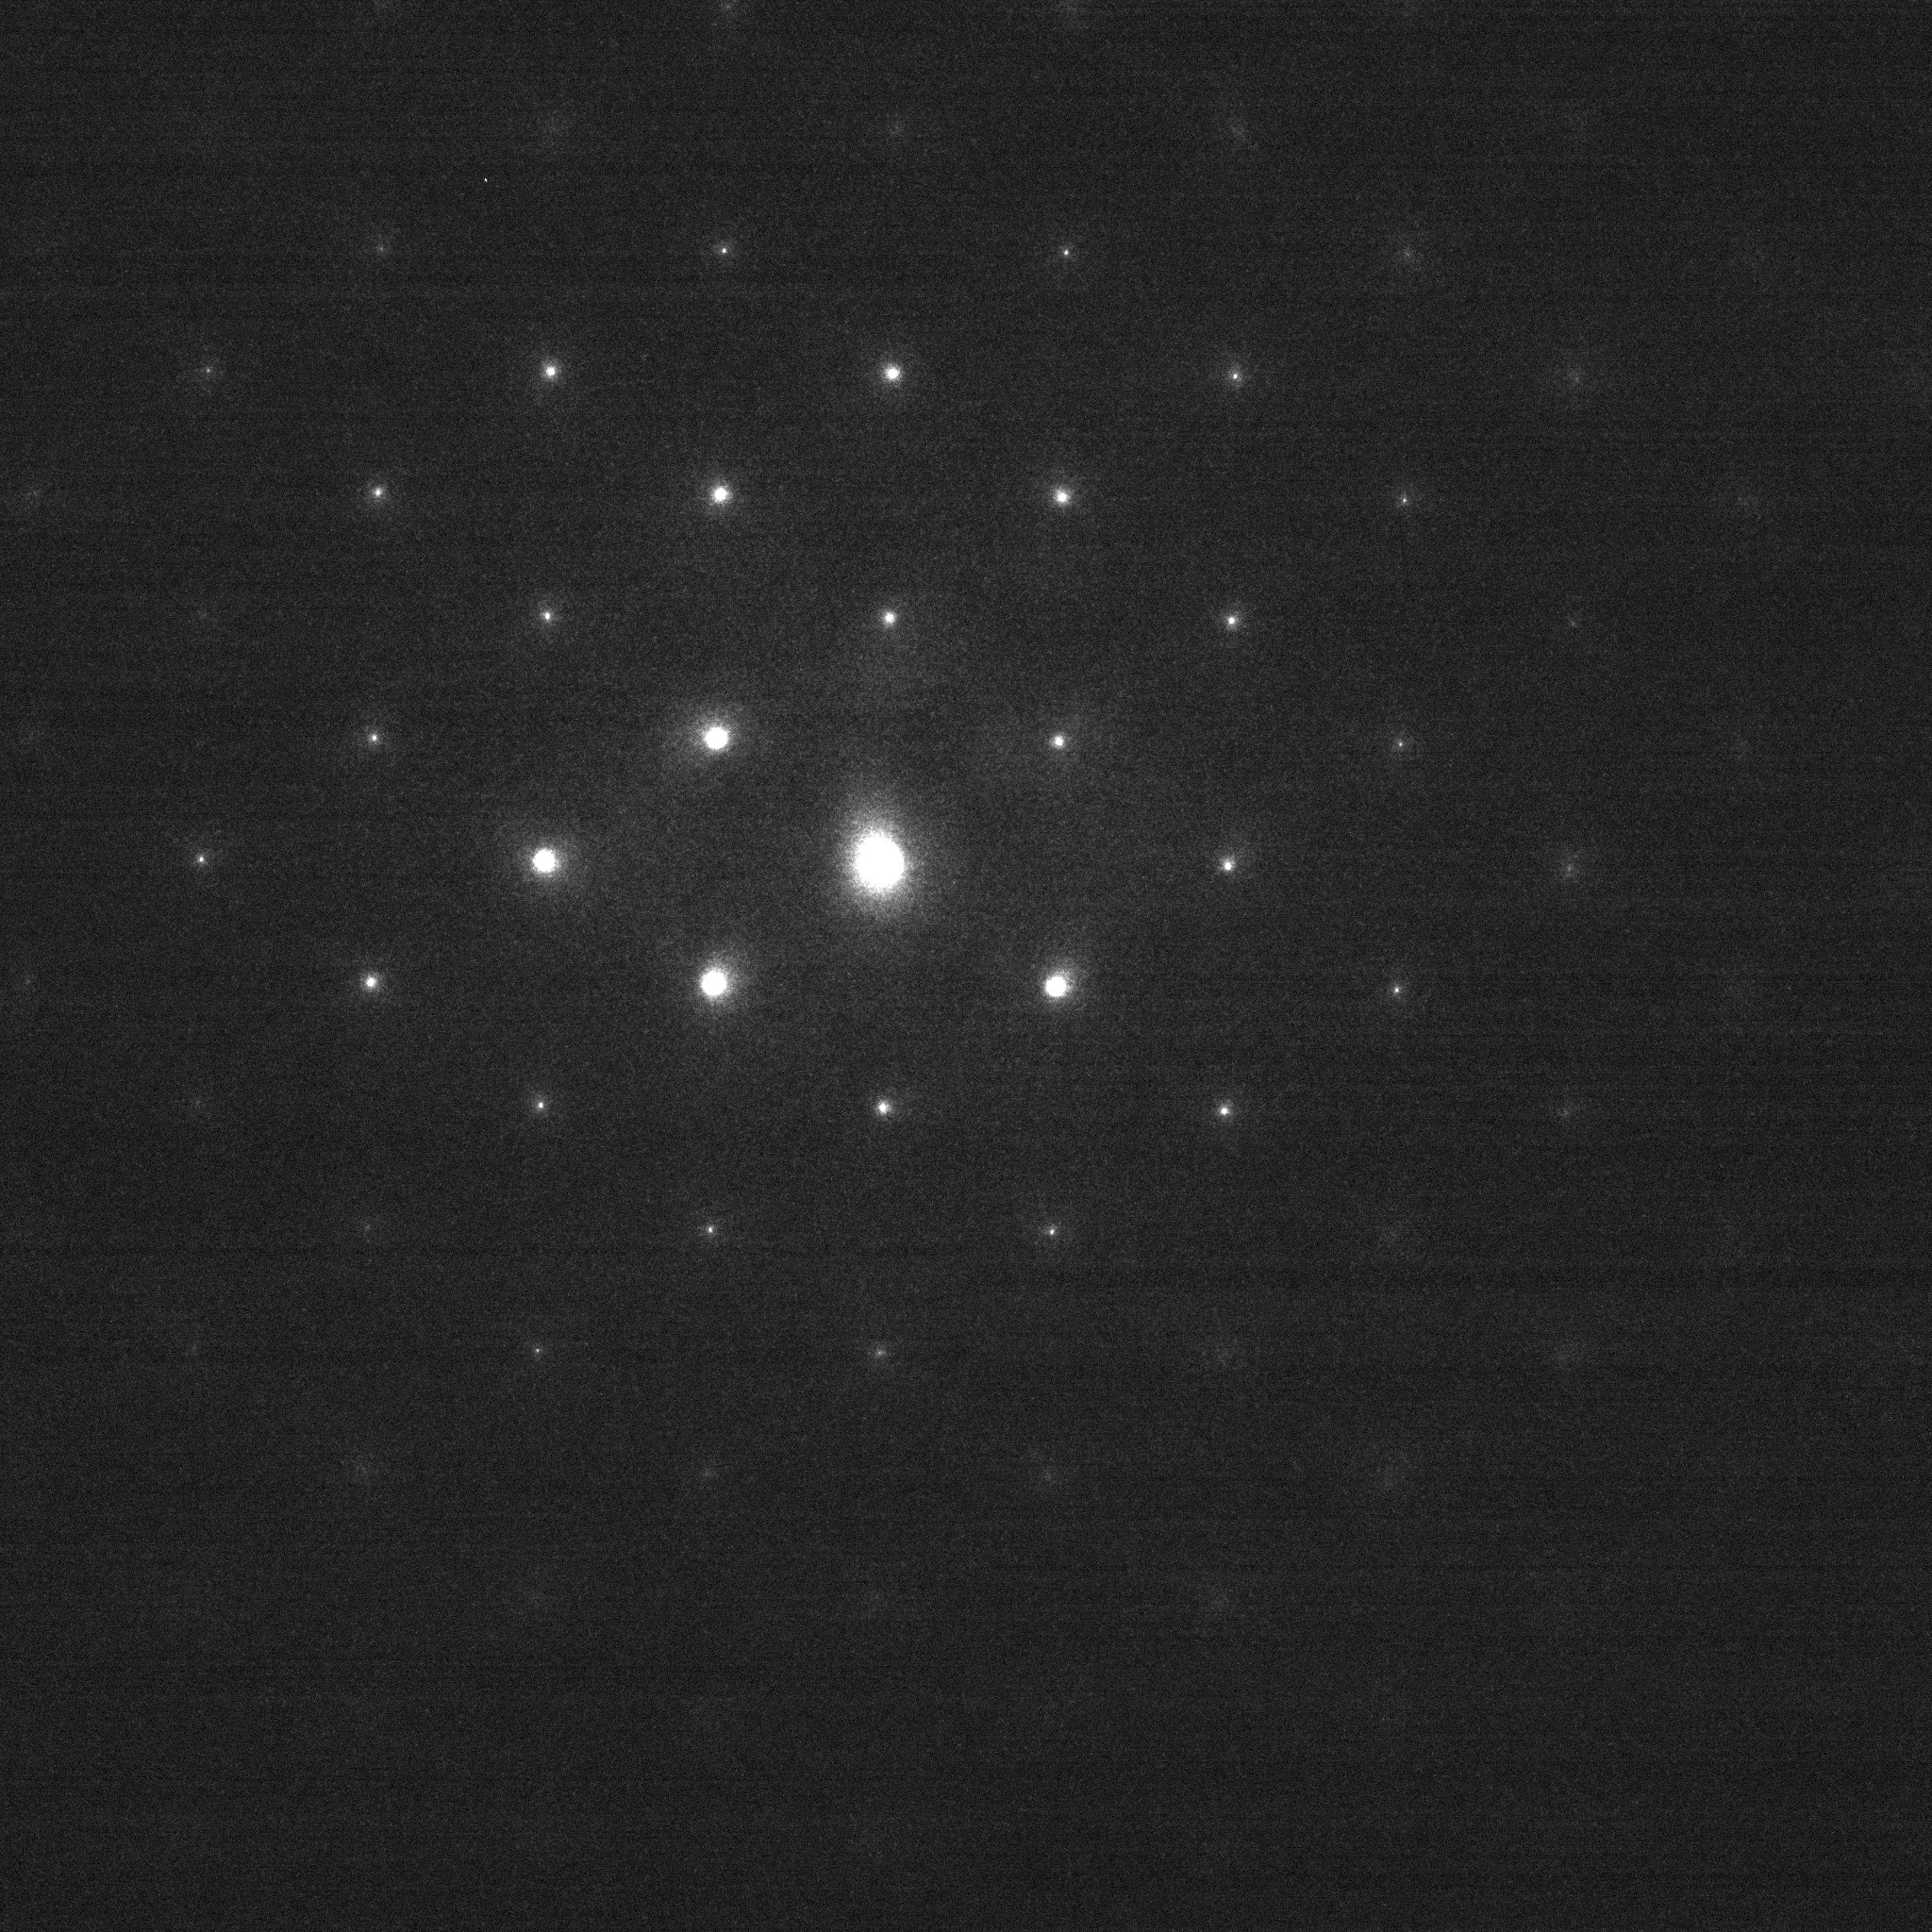
\includegraphics[width=\textwidth]{Grundlagen&Beugung/Eigenprobe_Beugungsbild_zonenachse1.jpg}
         \caption{Beugungsbild}
         \label{EPBB}
     \end{subfigure}
     \hfill
     \begin{subfigure}[b]{0.49\textwidth}
         \centering
         
\includegraphics[width=\textwidth]{Grundlagen&Beugung/Eigene_Probe_Schooeneaufnahme.jpg}
         \caption{Im Fokus}
         \label{EPFokus}
     \end{subfigure}
     \hfill
     \begin{subfigure}[b]{0.49\textwidth}
         \centering
         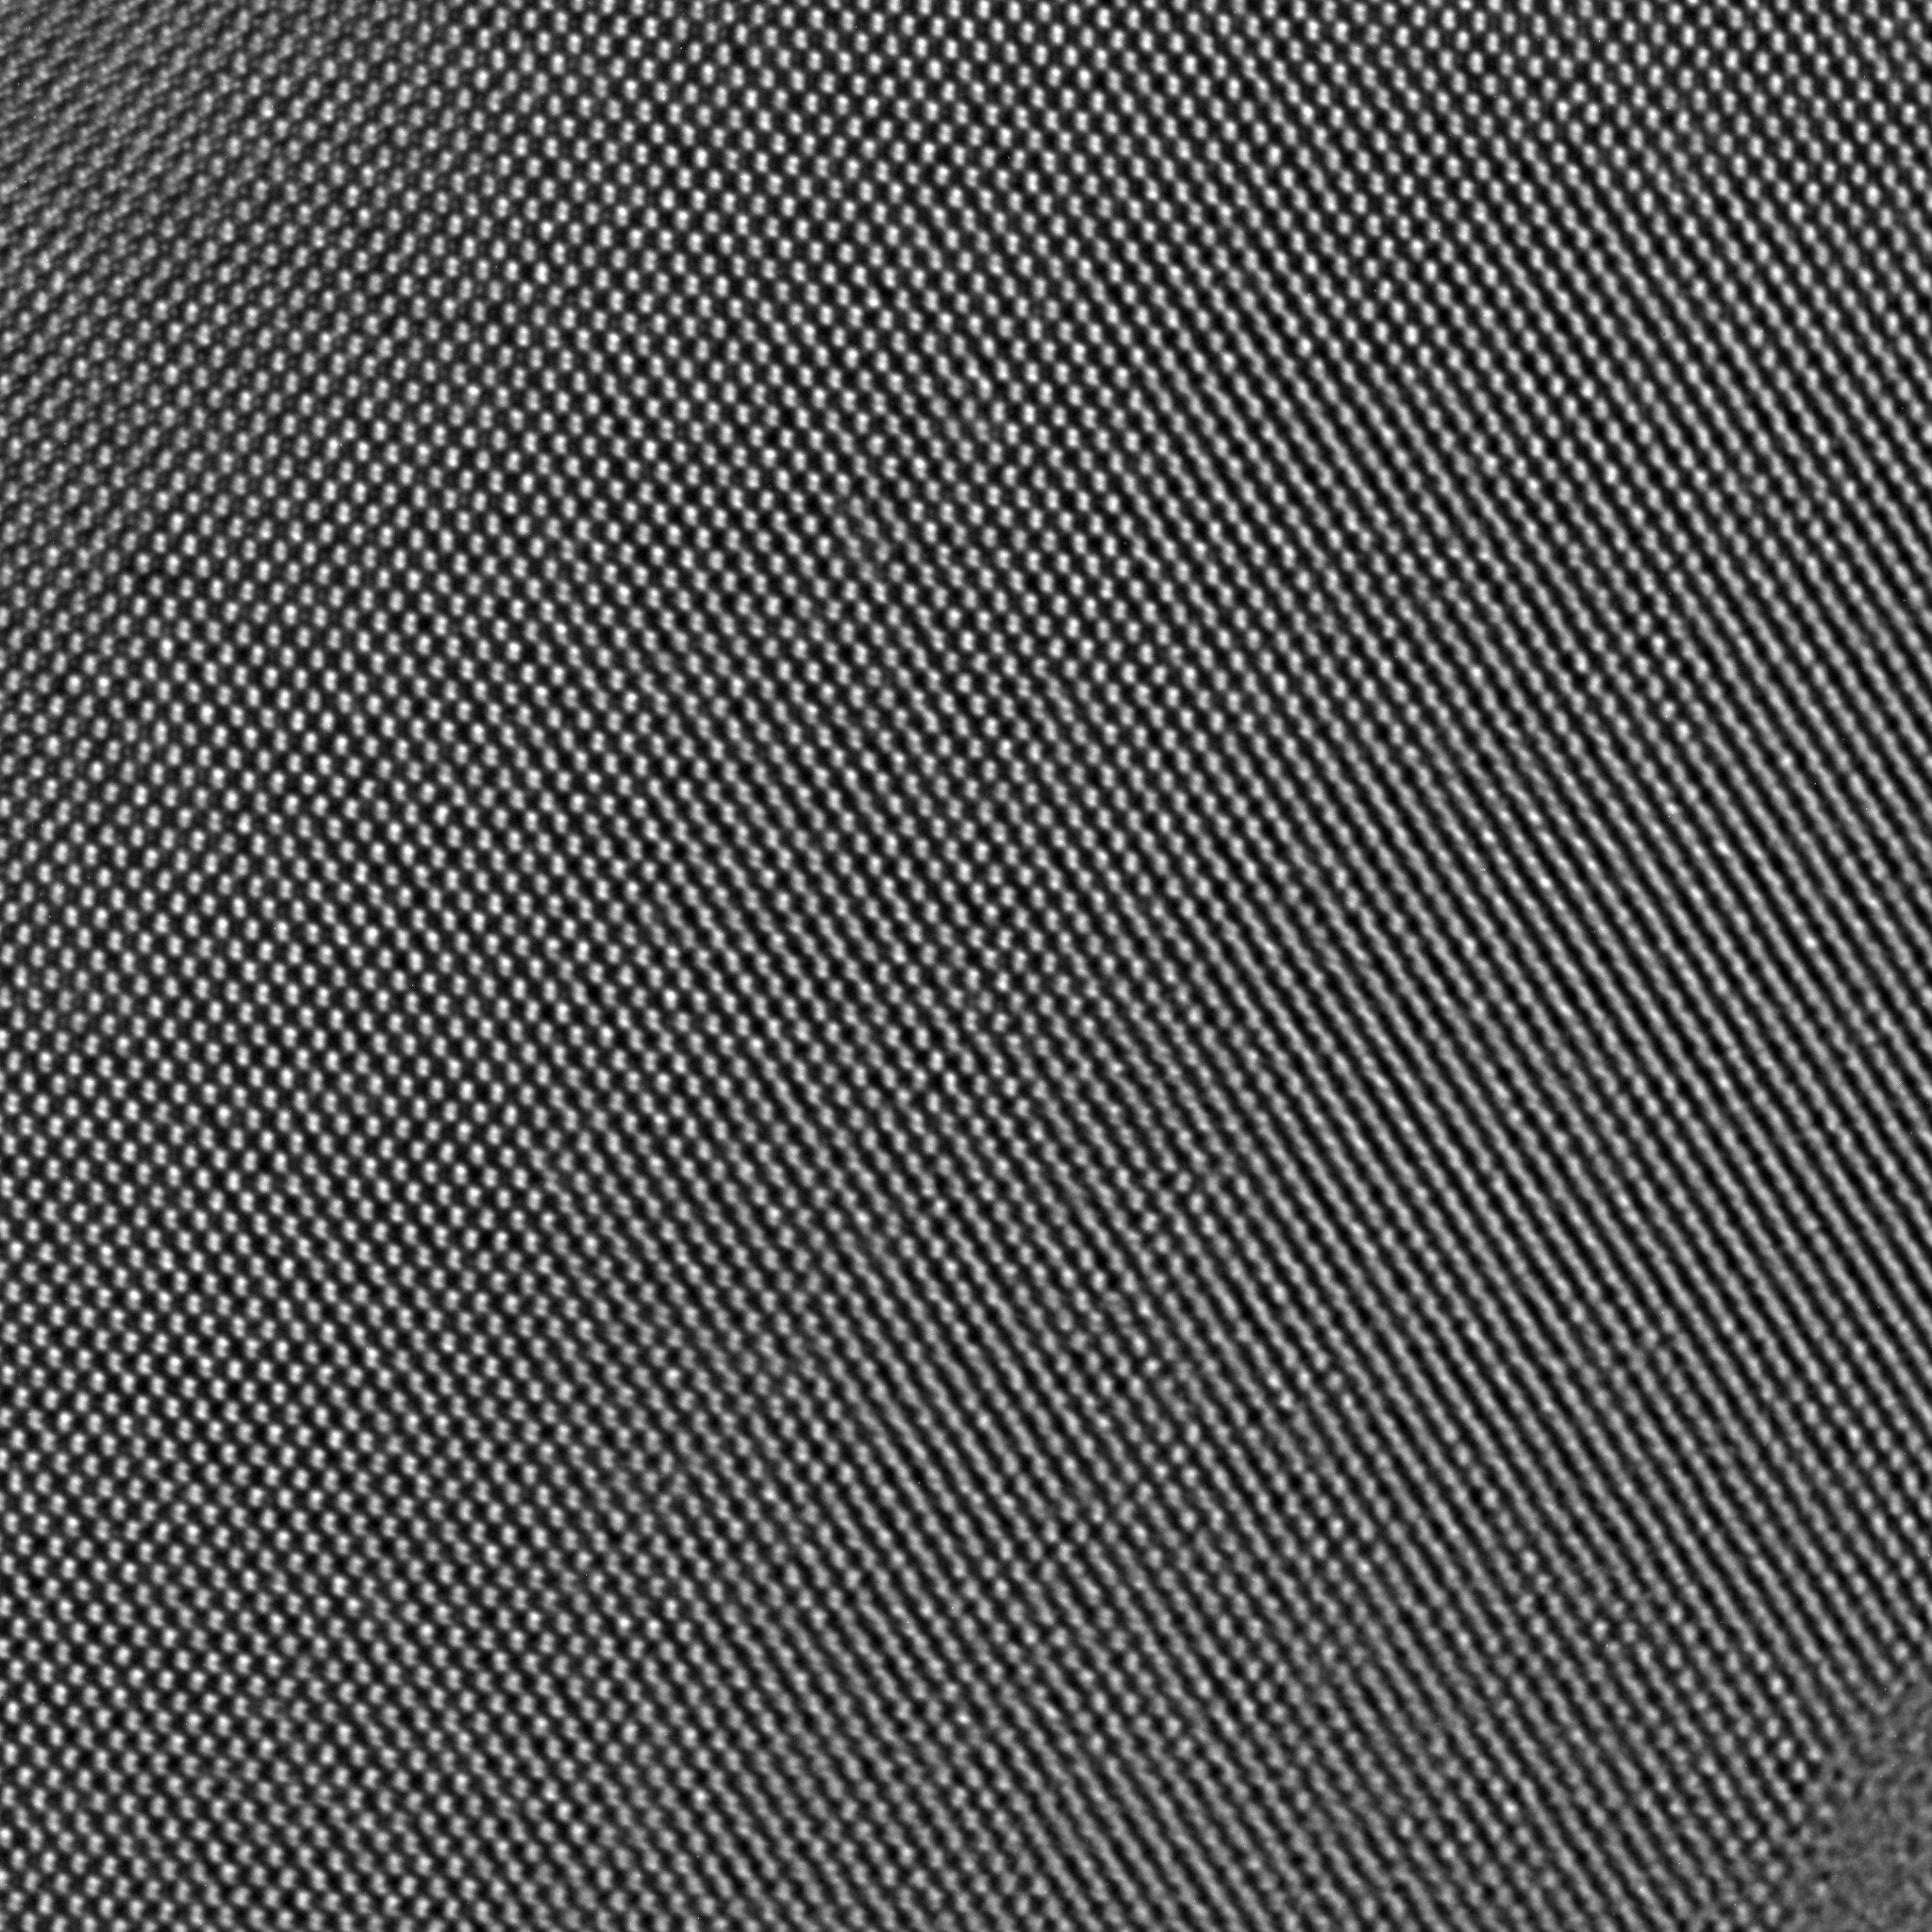
\includegraphics[width=\textwidth]{Grundlagen&Beugung/Eigene_Probe_Unterfokus2.jpg}
         \caption{Unterfokus}
         \label{EPUnterfokus}
     \end{subfigure}
     \hfill
     \begin{subfigure}[b]{0.49\textwidth}
         \centering
         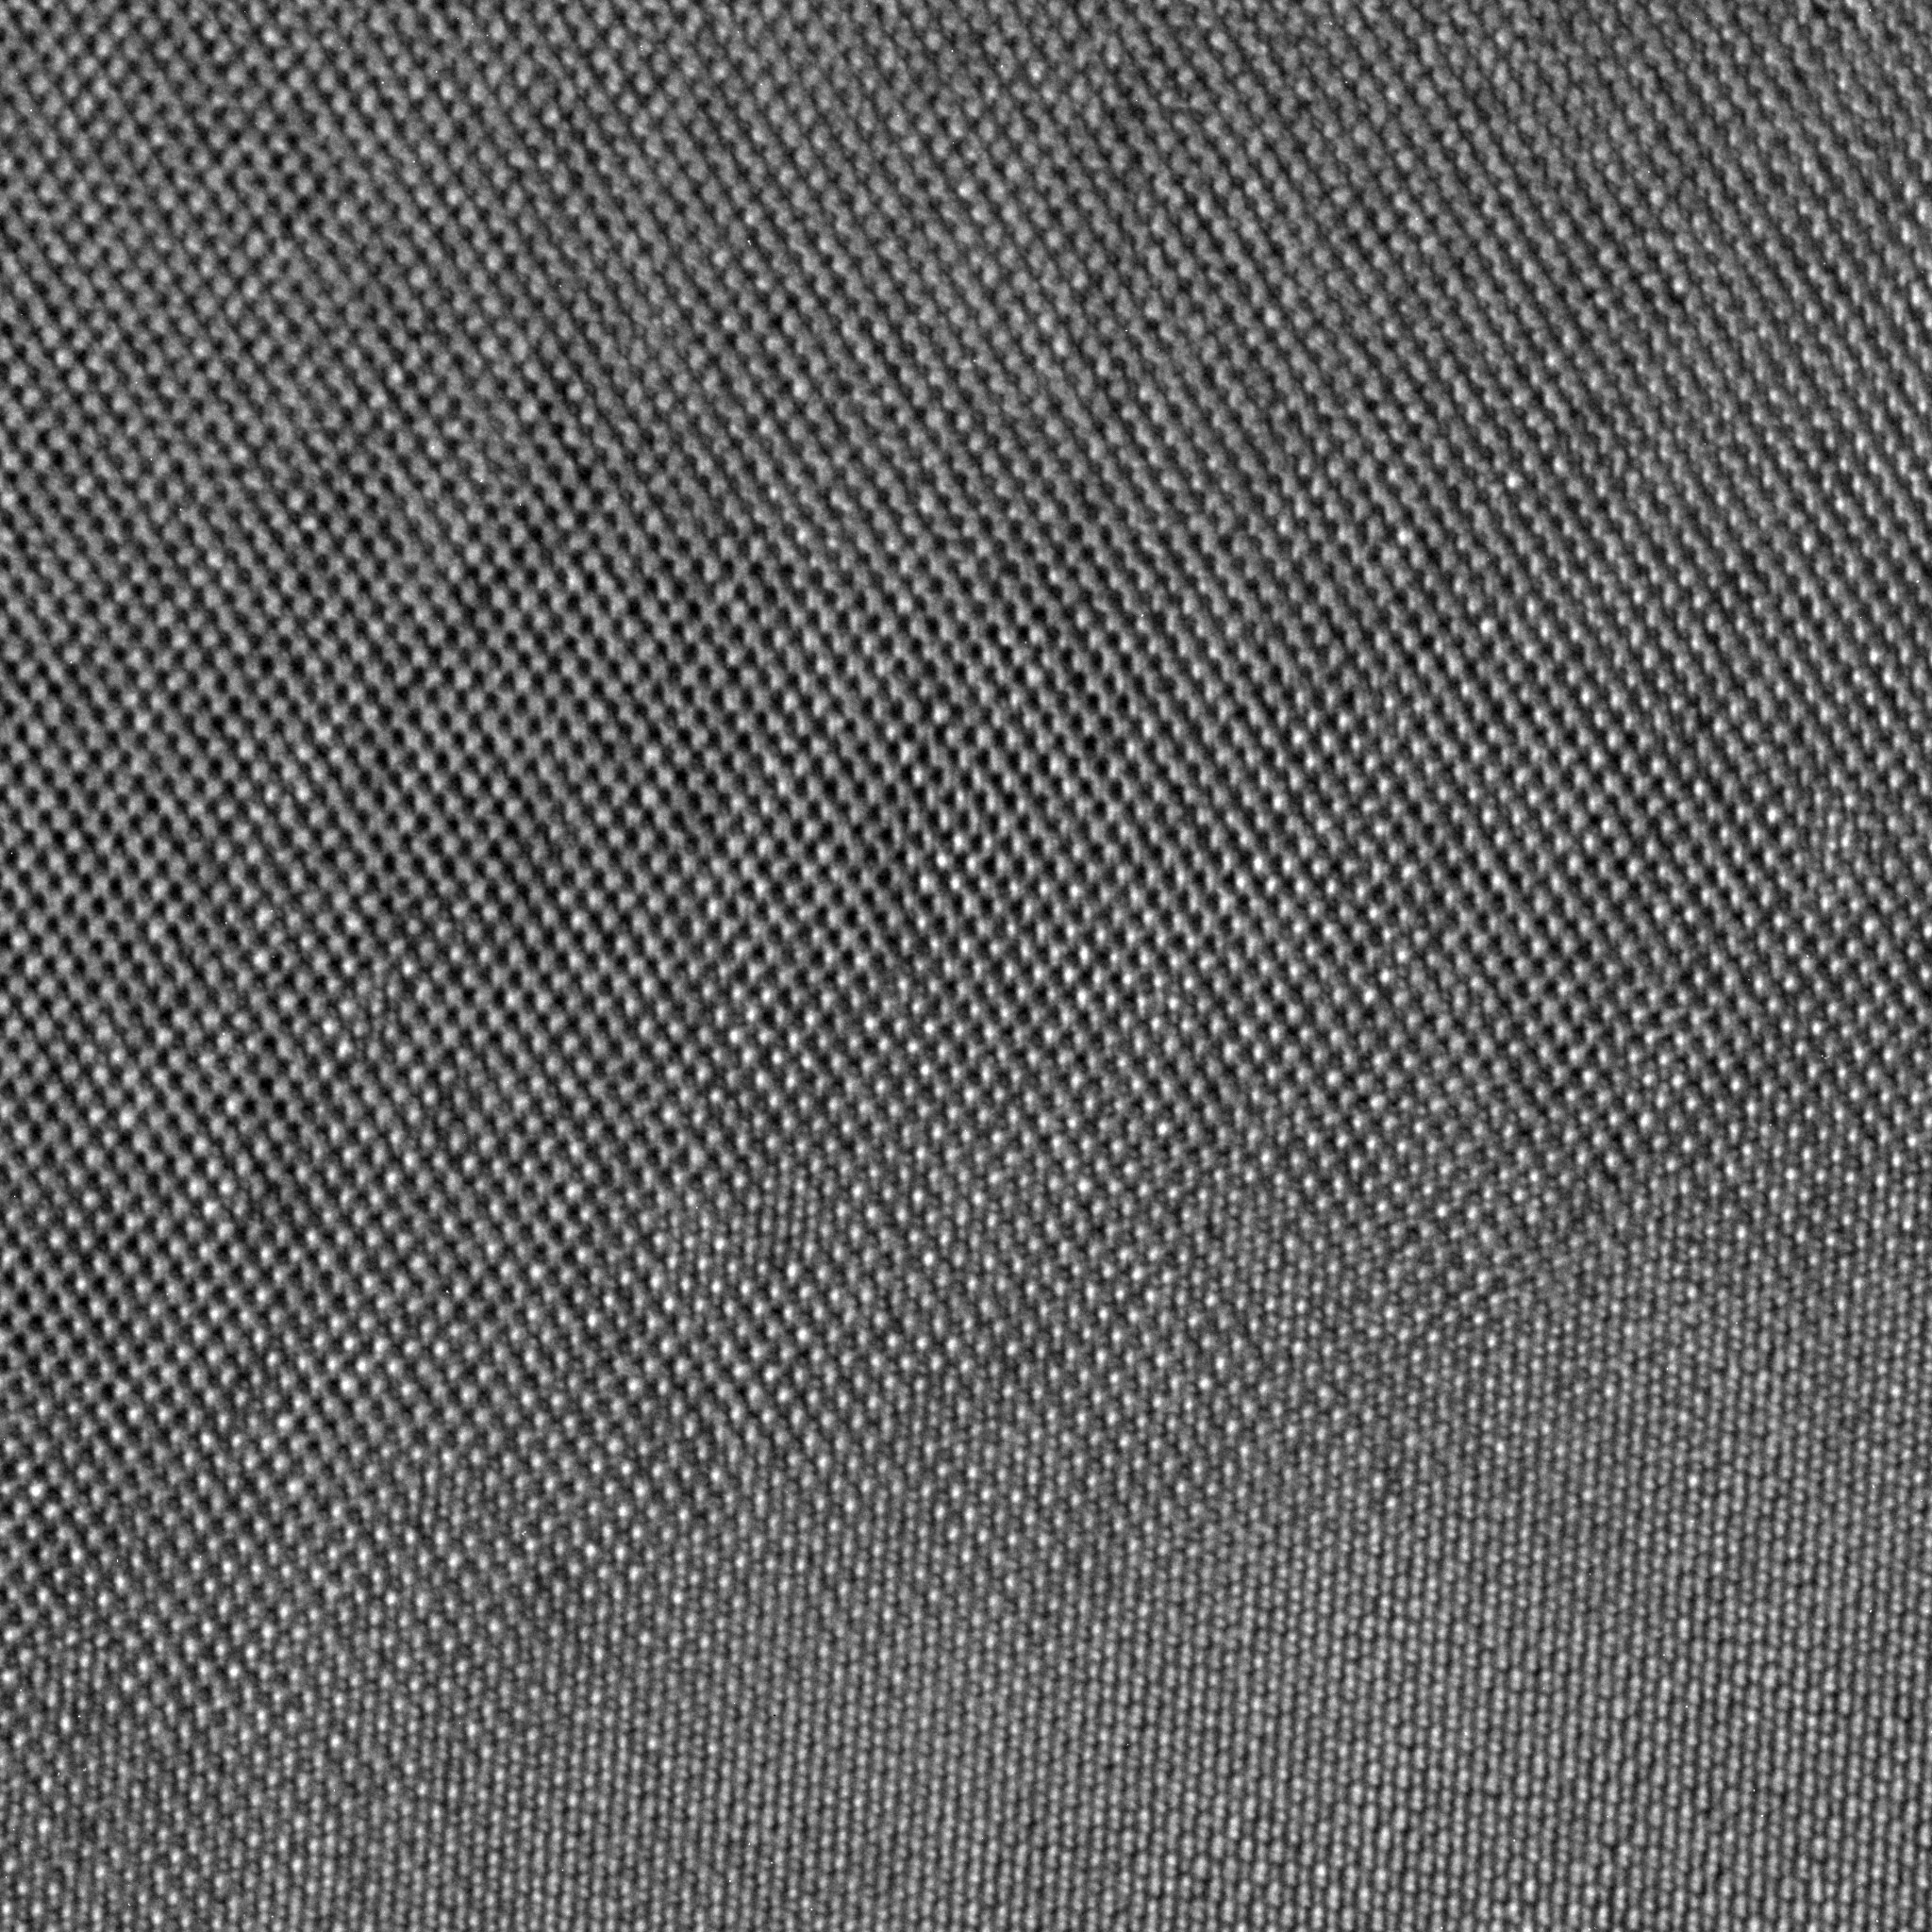
\includegraphics[width=\textwidth]{Grundlagen&Beugung/Eigene_Porbe_Ueberfokus.jpg}
         \caption{Überfokus}
         \label{SPÜberfokus}
     \end{subfigure}
        \caption{HRTEM Aufnahmen der selbst angefertigten Probe. Mir Beugungsbild, Unterfokus und Überfokus. Beugungsbild Aufnahme entlang der Zonenachse (110), Gemessene Reflex Abstände zum nullstrahl: \(R1(200) = 7,148, R2(220) = 9.810 und R3(111) = 6.450\).}
        \label{EigeneProbe}
\end{figure}

Mit dem Beugungsbild wurde zunächst versucht die Zonenachse zu identifizieren, hierfür wurden mit Hilfe der Software „ImangeJ“ die Distanzen vom Nullstrahl zu den anliegenden Reflexen der XYZ Richtungen gemessen. \\
%R1=7,148/2 (3,574), Y = 9.810/2 (4,905), Z = 6,450/2 (3,225)
Mit Hilfe des Struktur Faktor Formel und dem Wissen das sie Probe ein GaAs Kristall ist, welcher eine FCC (Face Centered Cubic) ist kann folgende Relation gefunden werden.
\[
    \frac{R_i}{R_j} = \frac{\sqrt{h_i^2+k_i^2+l_i^2}}{\sqrt{h_j^2+k_j^2+l_j^2}}
.\]
Dabei können nur Reflexe entstehen wenn hkl alle grade oder ungerade Werte haben, bei gemischten indeces ist der Strukturfaktor 0.
\[
    z.B. = 000, 111, 200, 220, 311, 222, 400, 331, 420, …
.\]
Mit einsetzen der gemessenen Längen und einsetzen verschiedener möglicher hkl Werte, wurden folgende Reflexe identifiziert.
\[
R_1 = (002), R_2 = (220), R_3 = (111) 
.\]
Die Zonenachse muss dementsprechend orthogonal zu diesen drei Achsen sein welche auf die [110] zutrifft.\\
Um auch aufnahmen an entlang anderen Zonenachsen zu erstellen wurde die Probe entlang der [001] Achse verkippt bis wieder ein zentriertes Beugungsbild erkennbar war. (siehe Abbildung \cref{EP2BB}).\\
Hierbei wurden die (020), (200) und (220) Reflexe beobachtet, so dass die Zonenachse nun bei [001] war.

\begin{figure}[htbp]
 \centering
 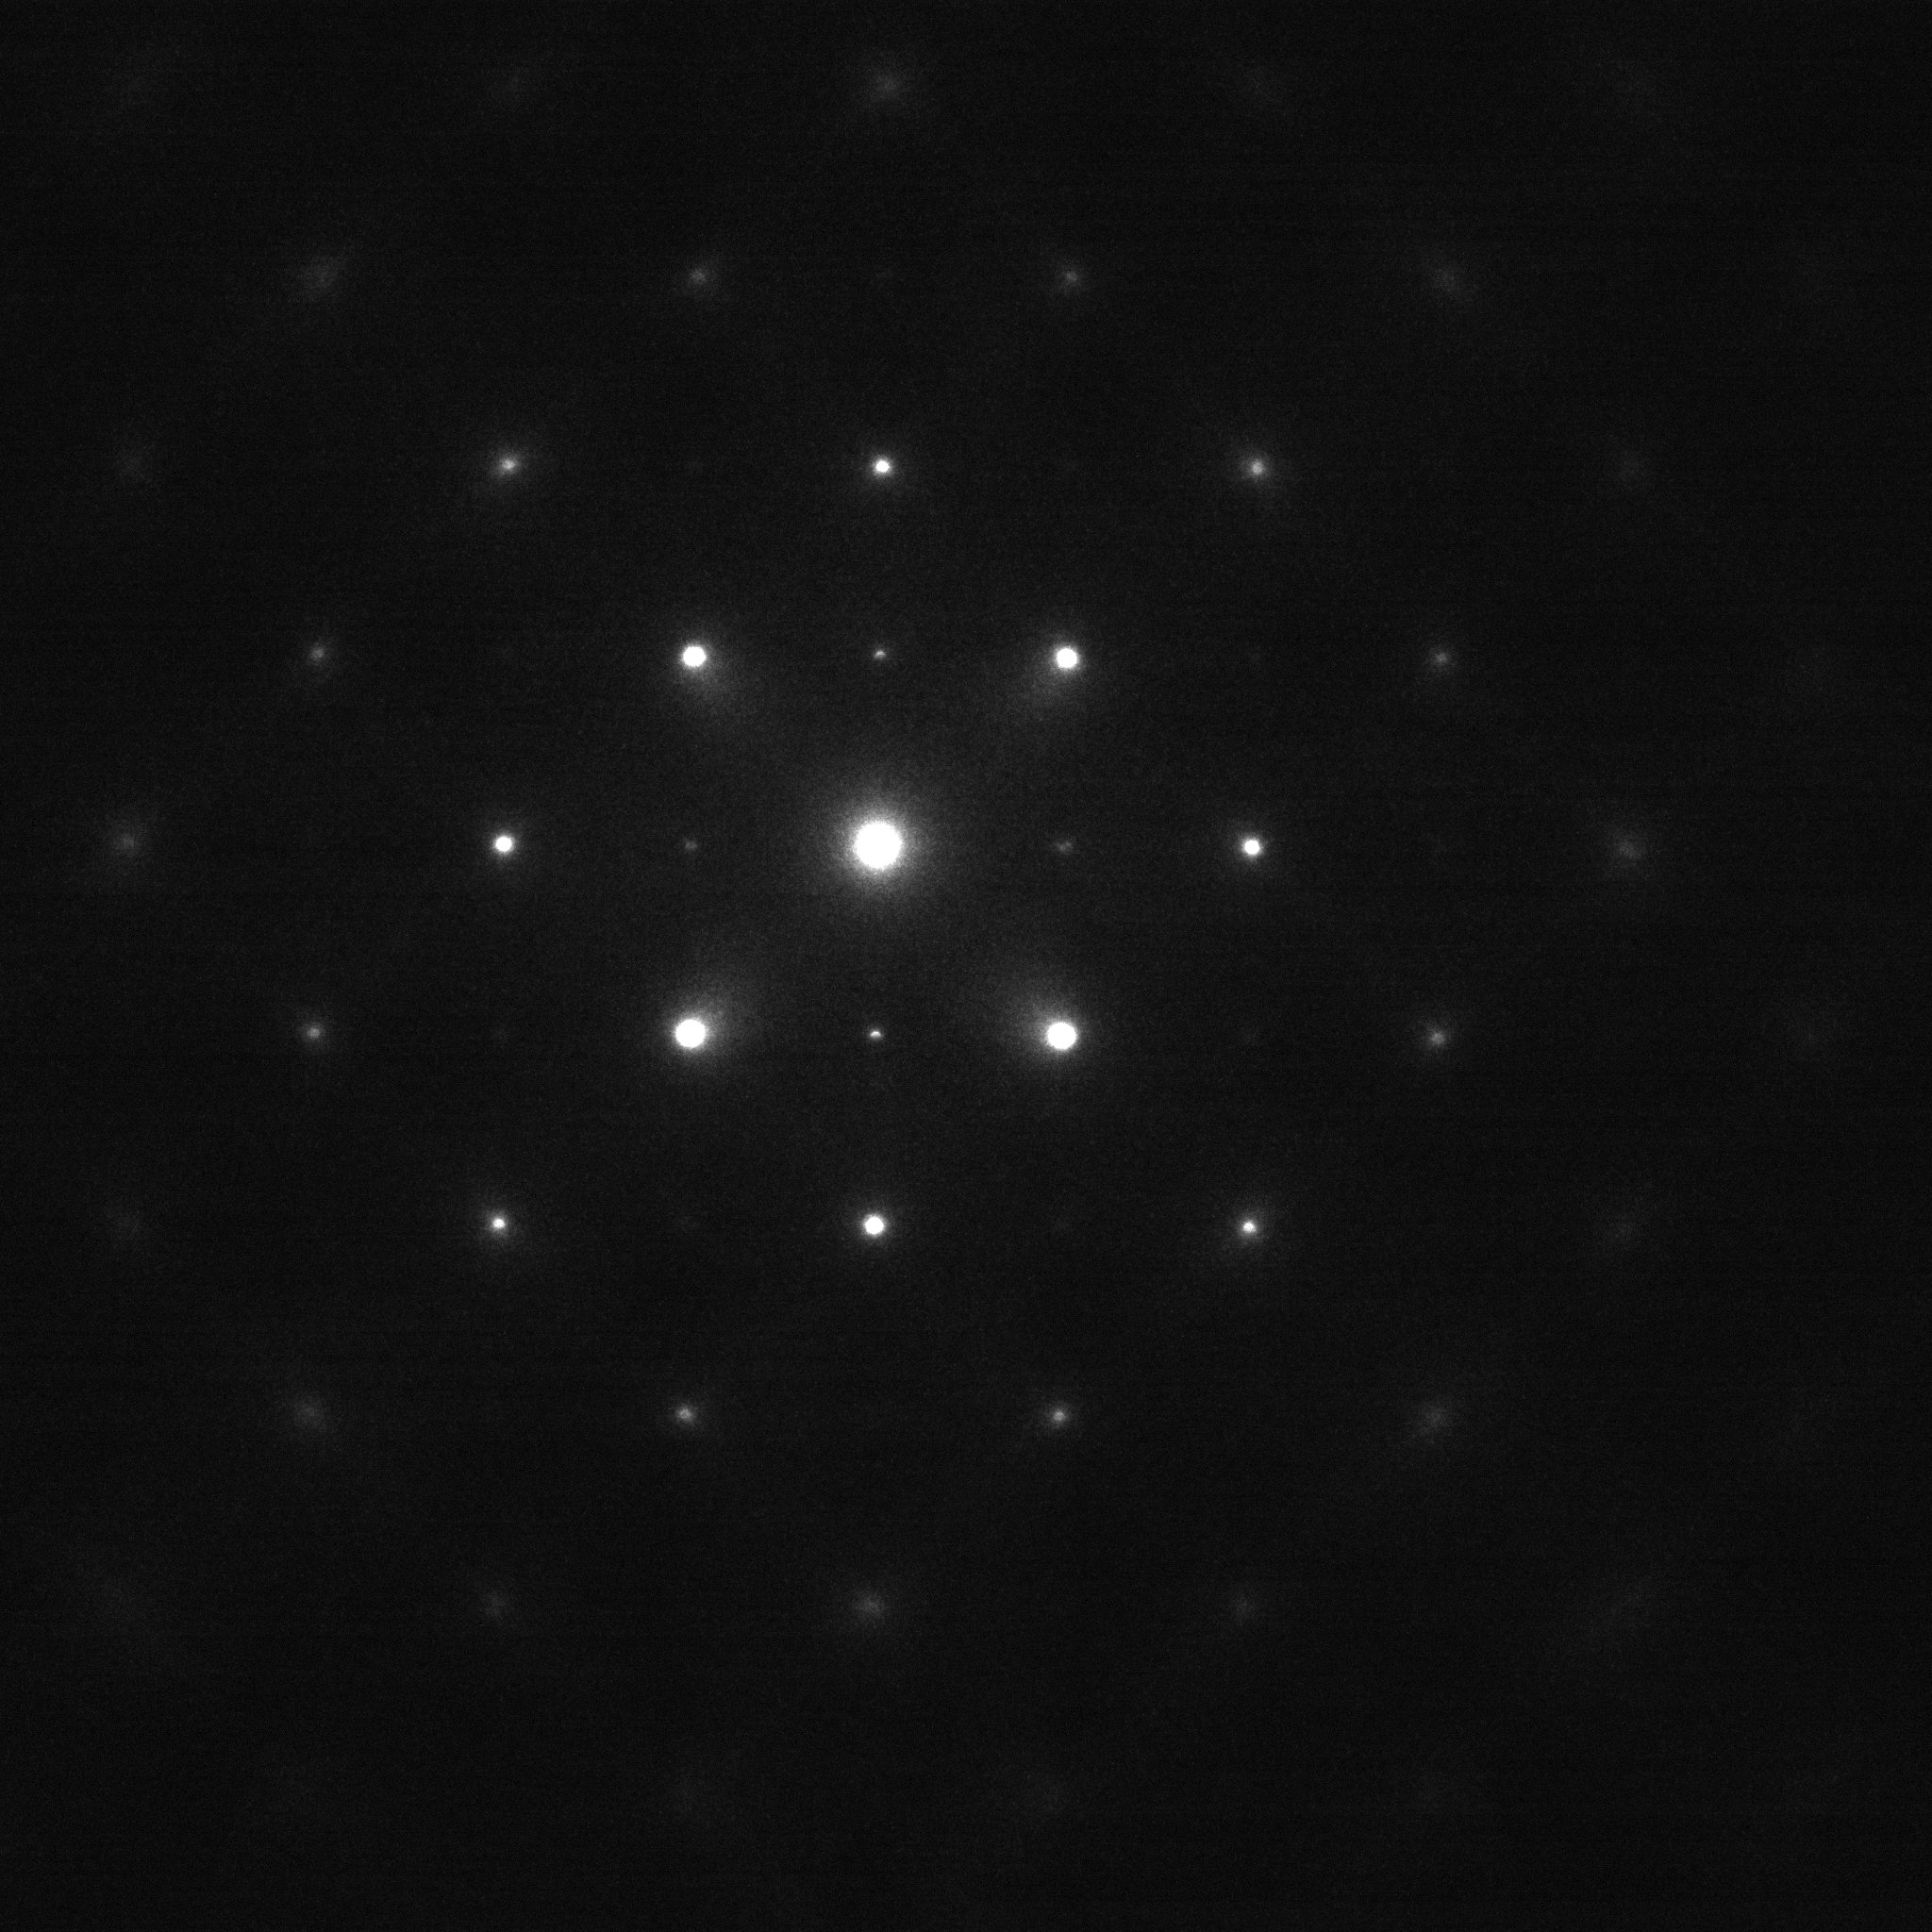
\includegraphics[width=0.7\textwidth]{Grundlagen&Beugung/Eigene_probe_Andere_seite_difraction.jpg}
 \caption[Beugungsbild(001)]{Beugungsbild Aufnahme entlang der Zonenachse (001), Gemessene Reflex Abstände zum nullstrahl: \( R_1(020)=7,086, R_2(220)= 6,98 und R_3(200)= 4,824 \).}
 \label{EP2BB}
\end{figure}

\subsubsection{CBED Aufnahmen}
CBED steht für „Convergent Beam Electron Diffraction“ dies bedeutet das wir im Beugung Modus einen Beleuchtungsstrahl haben der nicht mehr wie zuvor parallel, sondern Konvergent die Probe beleuchtet. Dabei weiten sich auch die Beugungsreflexe zu scheiben auf. Bei weiterer Aufweitung können die beugungsscheiben überschneiden und miteinander interferieren, dadurch werden die Kikuchi Lienen besonderes sichtbar.  Mit Hilfe von CEBD können mehrfachstreuengen der HOLZ Linien an dicken Proben abgebildet werden. Die Symmetrie des Kristals kann untersucht werden. Durch die Symmetrie der Beugungsbilder kann eine Chemische Sensitivität erreicht werden. An bestimmten Zonenachsen können Atome Positionen bestimmt werden.\\
Eine Reihe von CBED aufnahmen der GaAs Probe ist unten aufgeführt, dabei wurde die Beleuchtung von parallel zu konvergent angepasst.

\begin{figure}
     \centering
     \begin{subfigure}[b]{0.3\textwidth}
         \centering
         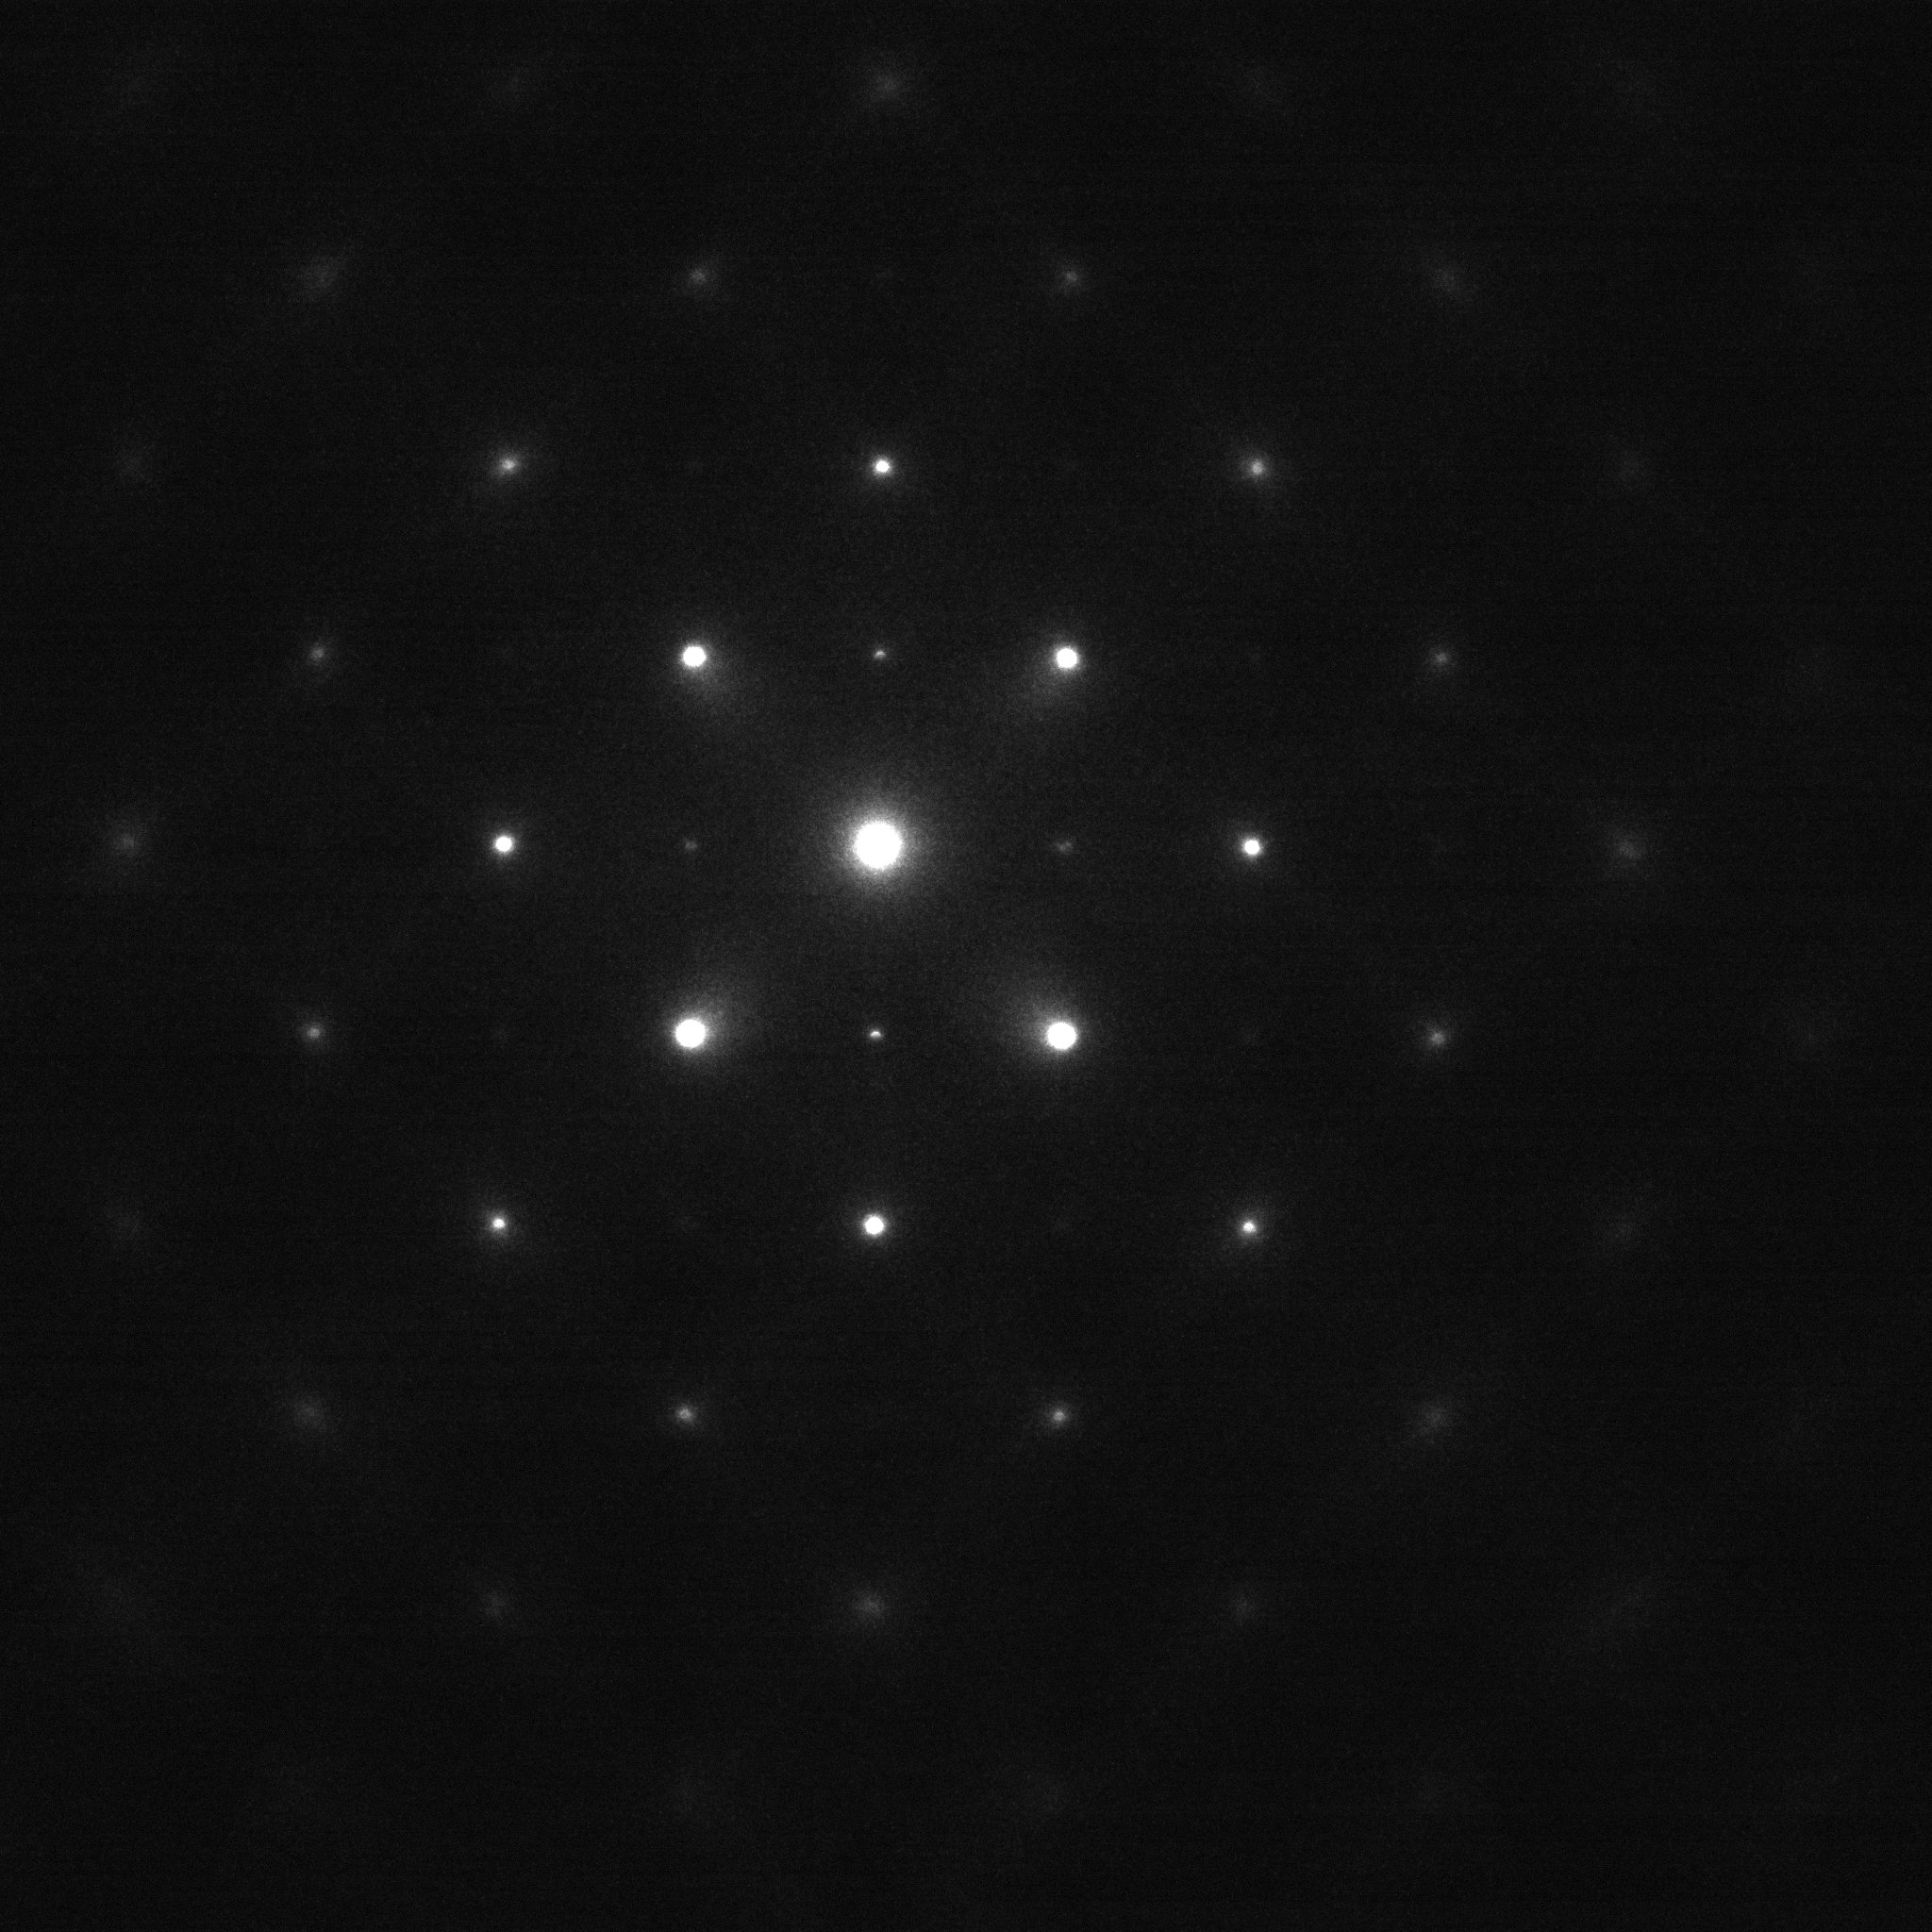
\includegraphics[width=\textwidth]{Grundlagen&Beugung/CBED1.jpg}
         \caption{Parallel}
         \label{CBEDP}
     \end{subfigure}
     \hfill
     \begin{subfigure}[b]{0.3\textwidth}
         \centering
         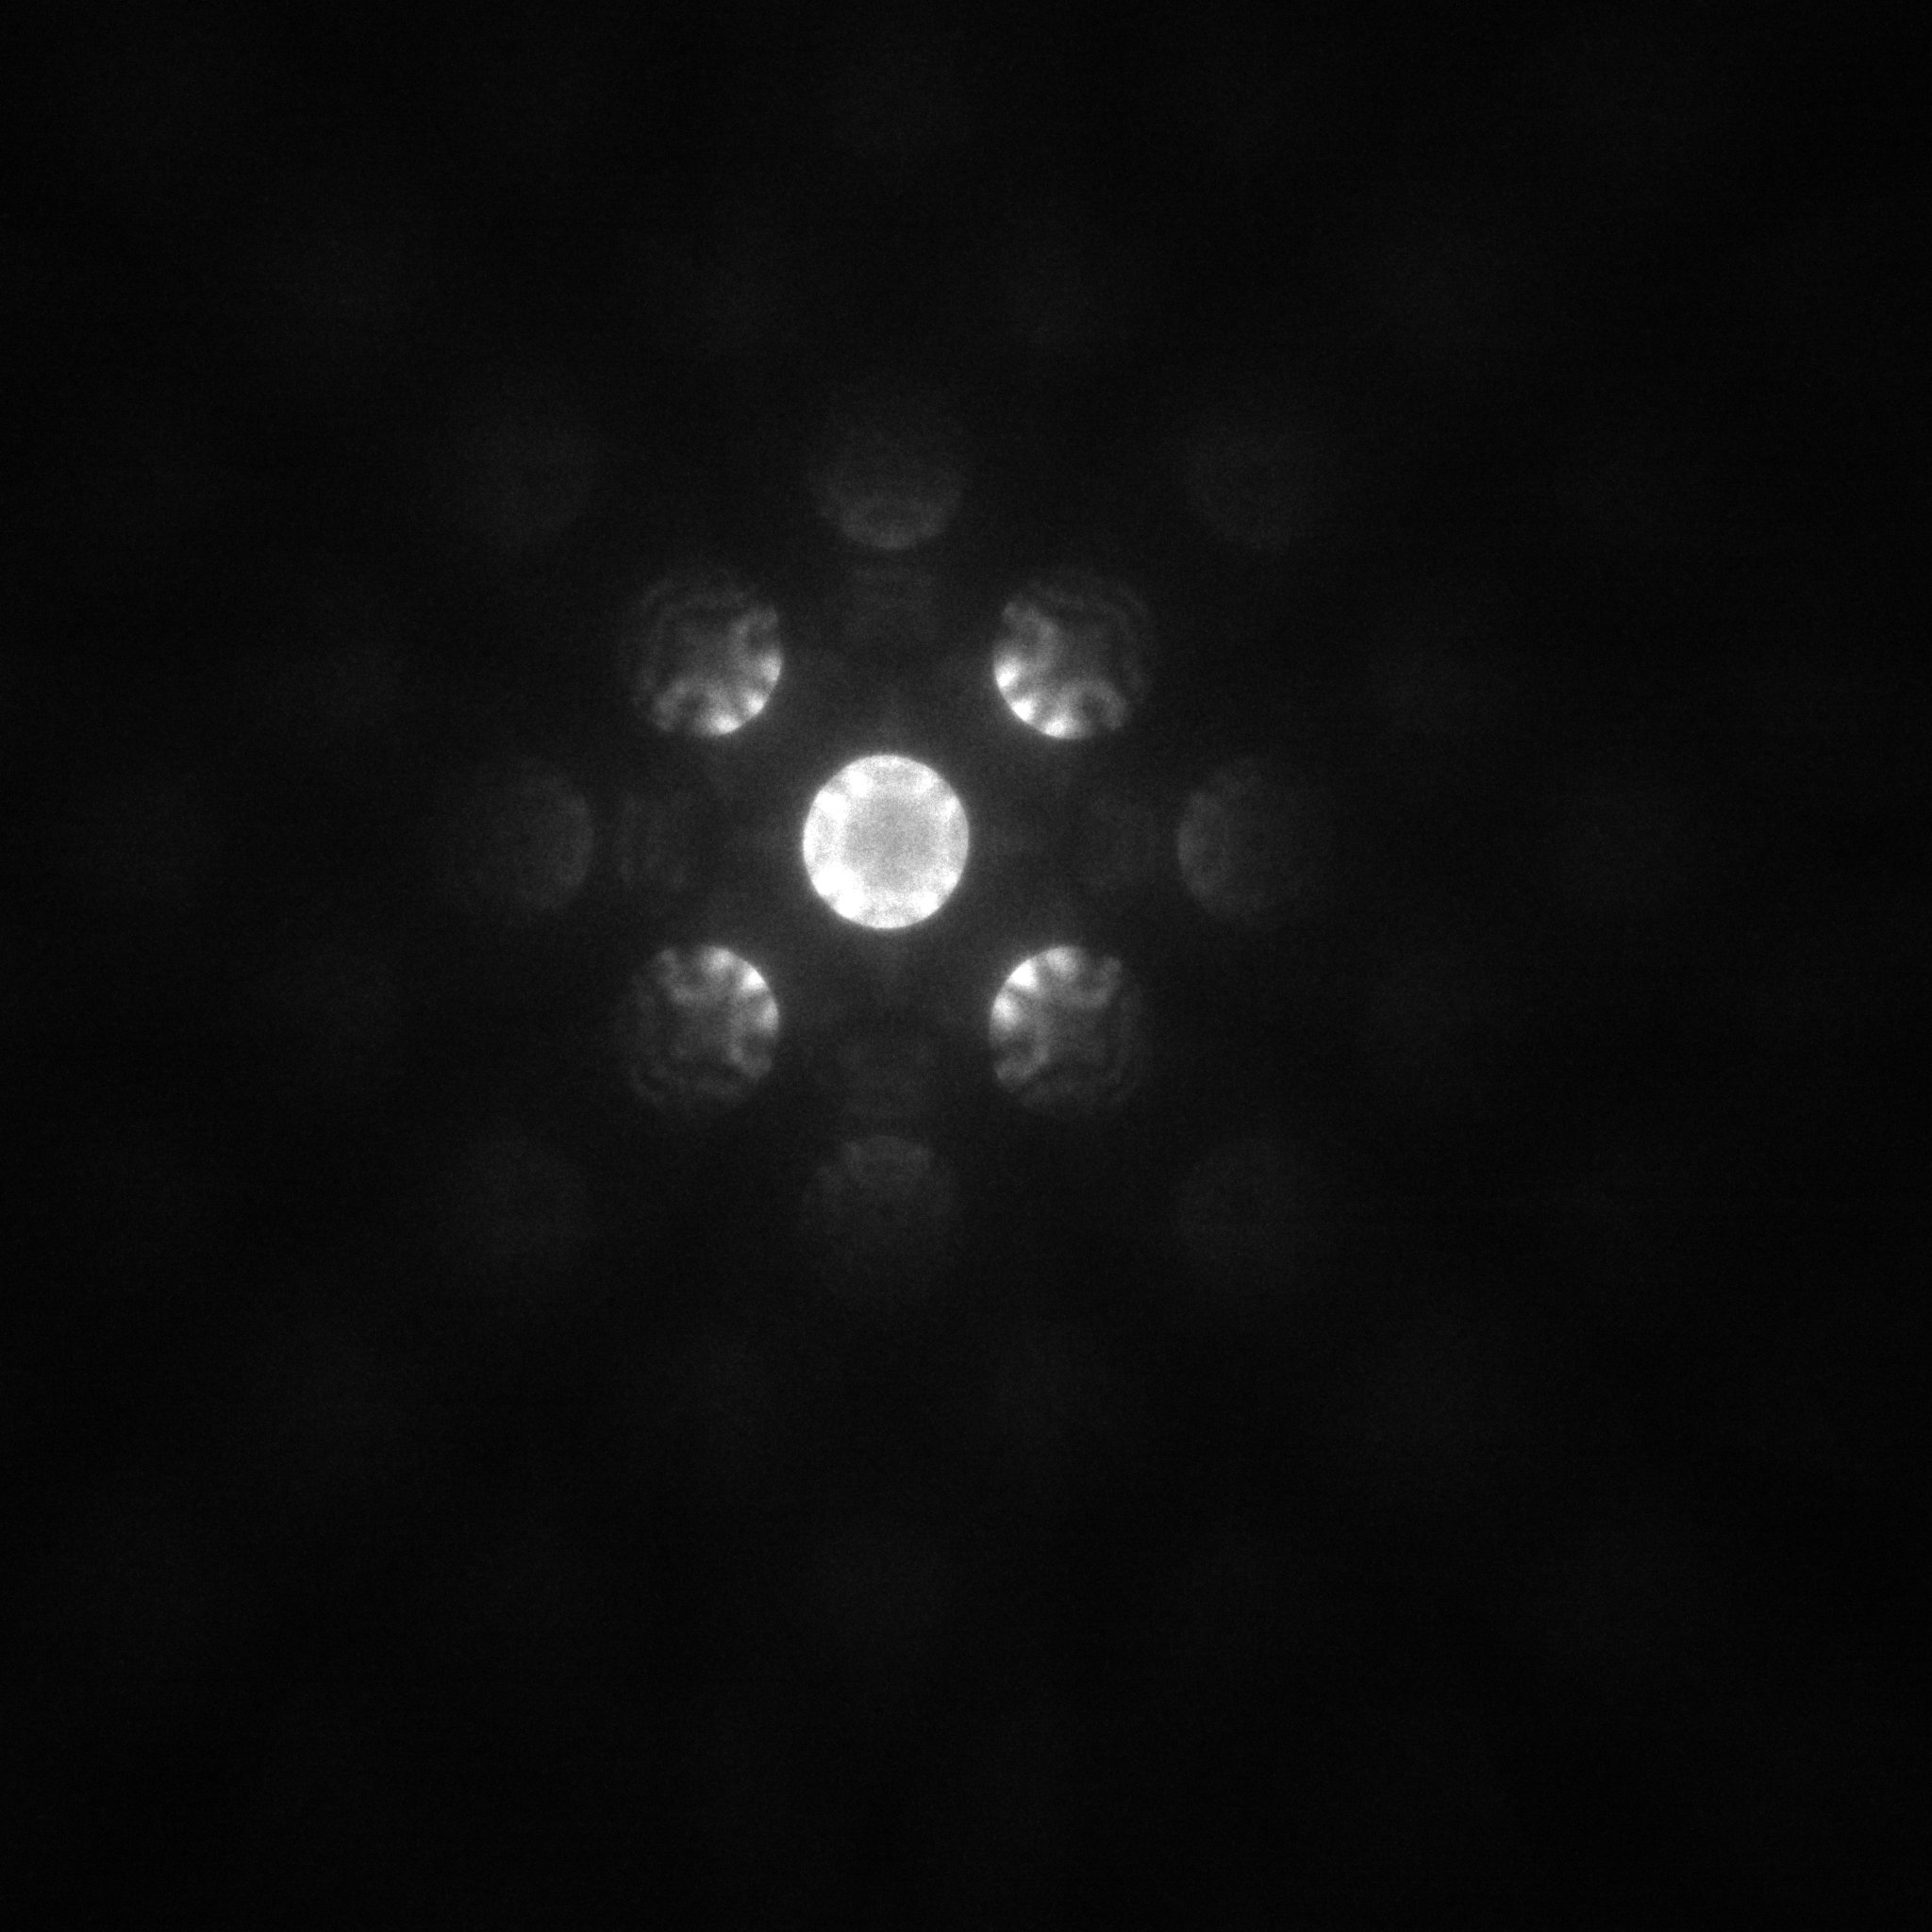
\includegraphics[width=\textwidth]{Grundlagen&Beugung/CBED2.jpg}
         \caption{semi-Konvergent}
         \label{CBEDSK}
     \end{subfigure}
     \hfill
     \begin{subfigure}[b]{0.3\textwidth}
         \centering
         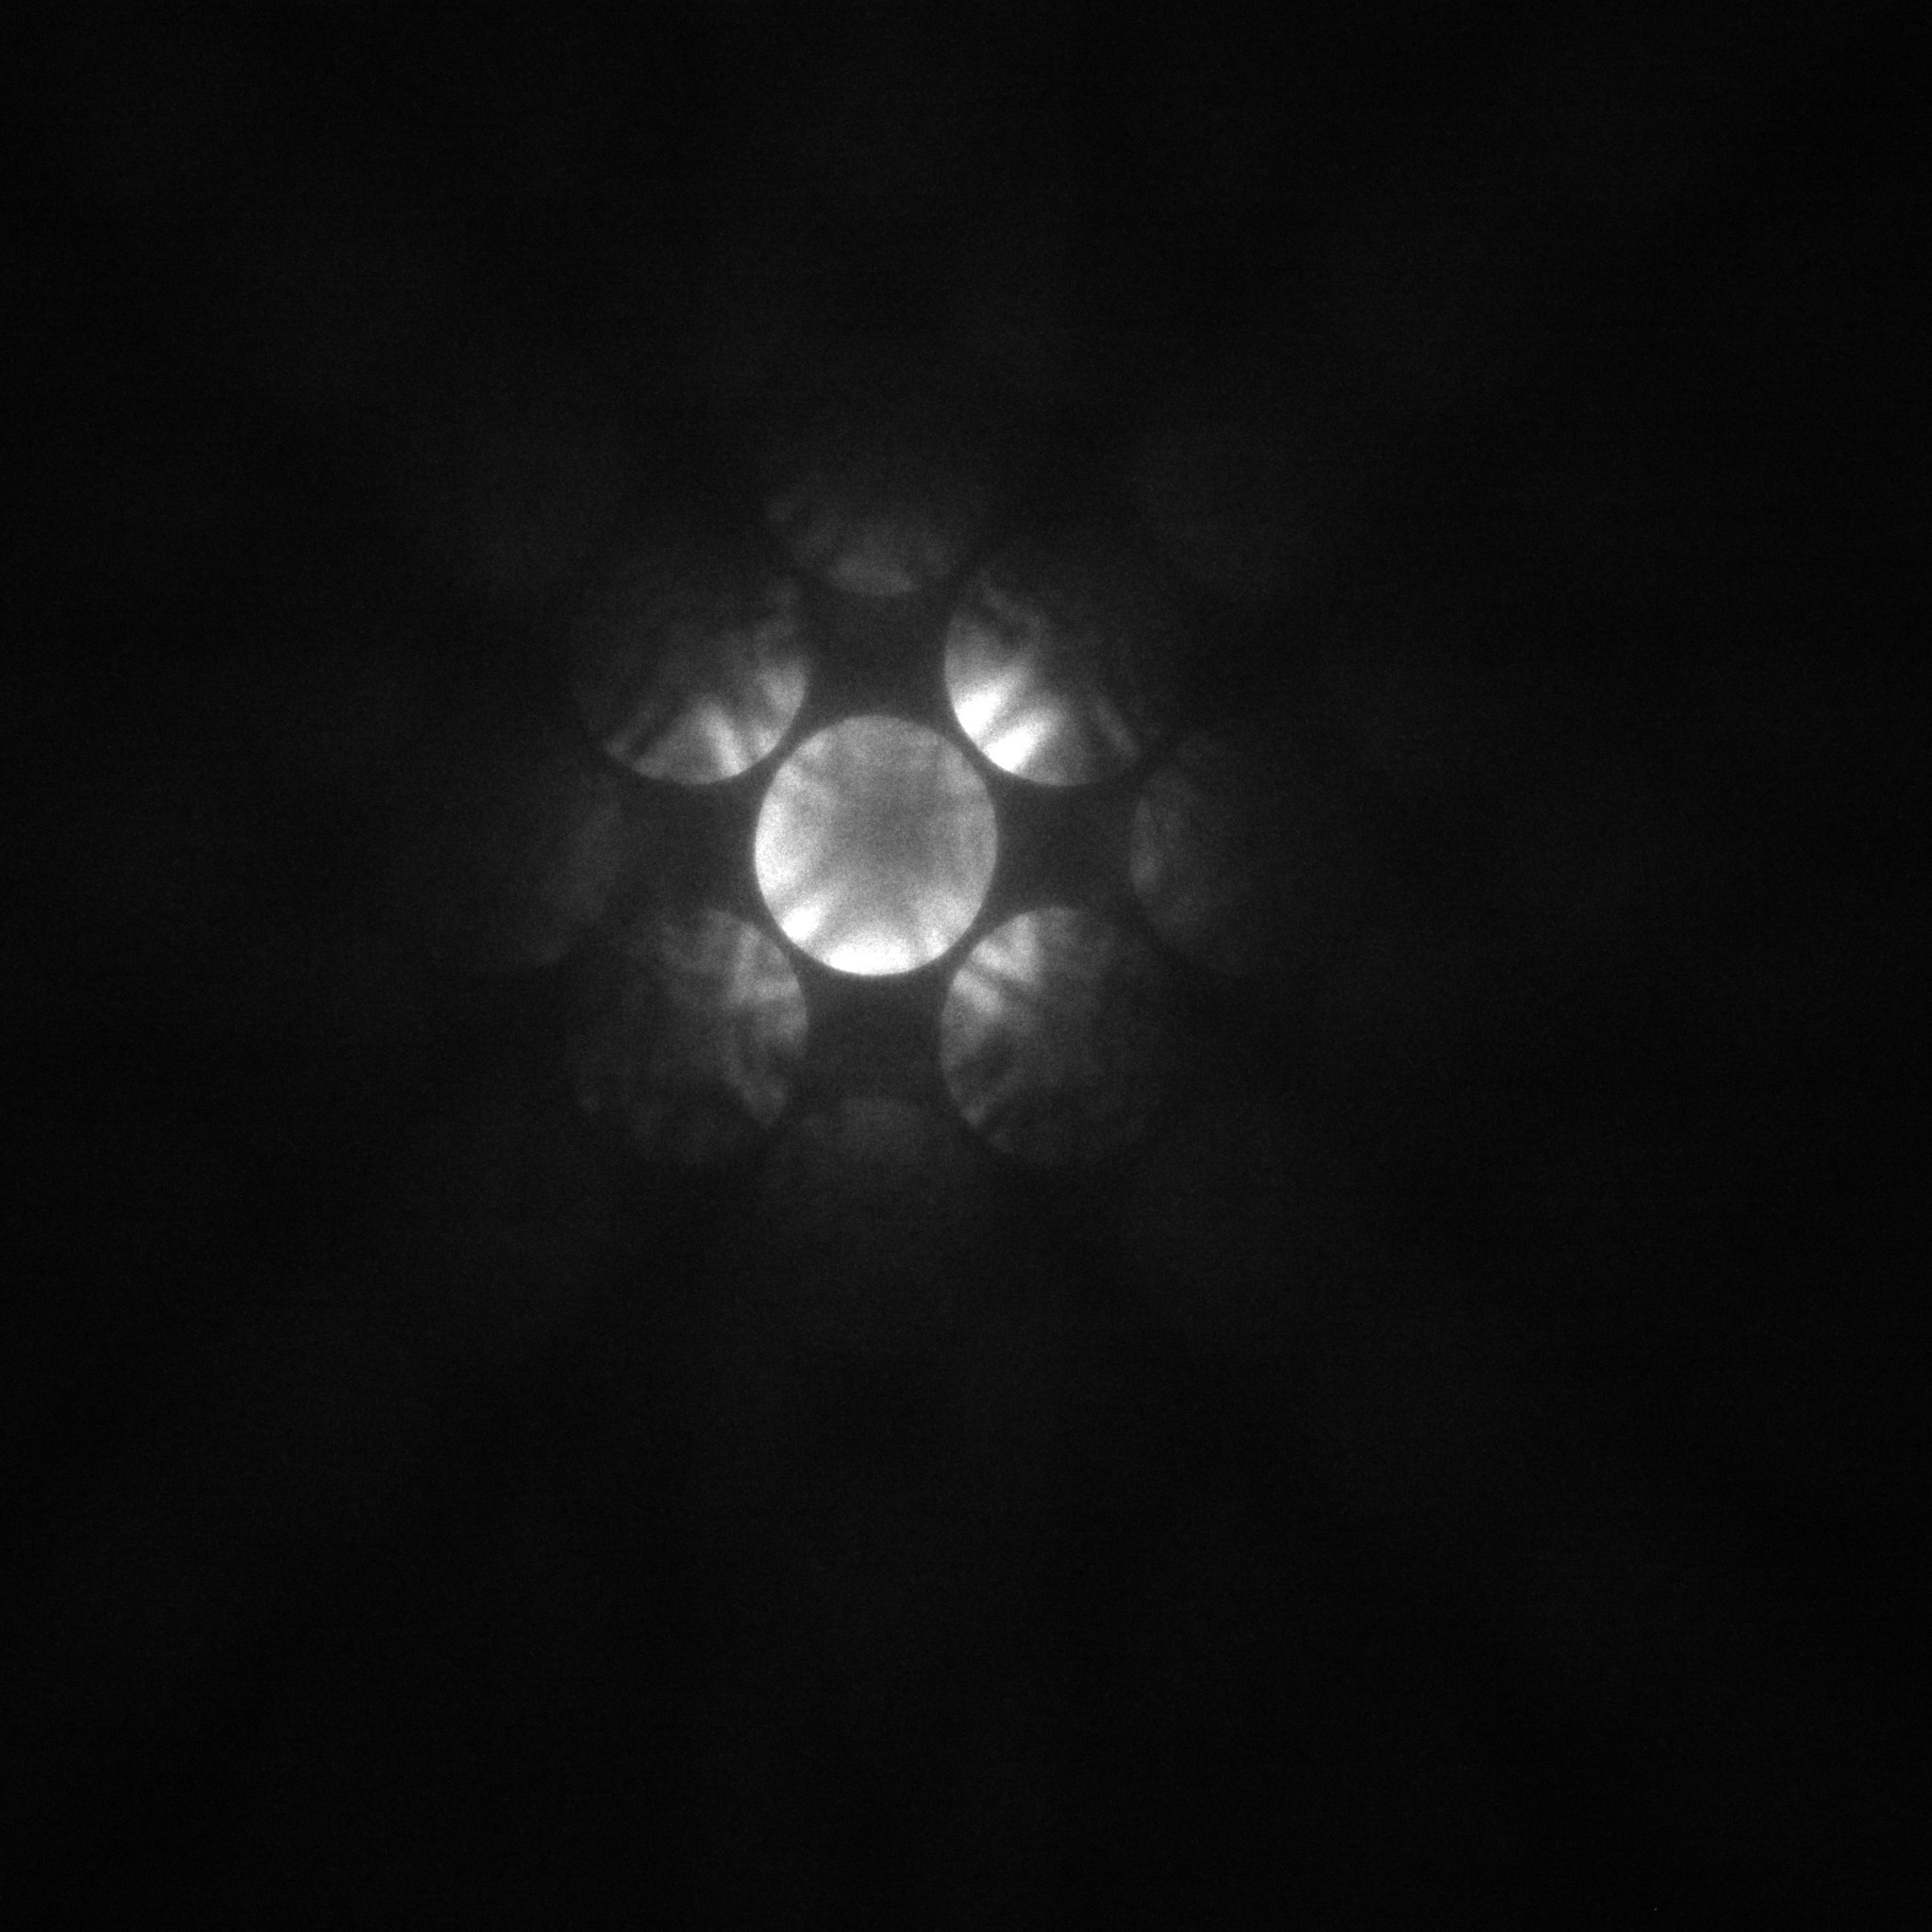
\includegraphics[width=\textwidth]{Grundlagen&Beugung/CBED3.jpg}
         \caption{Konvergent}
         \label{CBEDK}
     \end{subfigure}
        \caption{CBED Aufnehmen der Selbst erstellten GaAs Probe mit verschiedenen Konvergenten Winkeln \(\alpha\)}
        \label{CBED}
\end{figure}

Die GaAs Probe wurde sich im HRTEM im Bildmodus noch etwas angeschaut, dabei sind Zwei Interessante Segmente von besondere Interesse gewesen. 
Zunächst ein Aluminiumbelt (siehe \cref{EPBF&DFAl}). Das Al Belt ist gut in der Hellfeld Aufnahme zu erkennen, da sie einen sehr hohen Kontrast zum GaAs hat, es ist der Dunkler Steifen auf an der Oberseite des Bild. Zusätzlich sind in dieser Aufnahme die Quantum Belts, Untere Seite, zu erkennen und die Klebe stelle an der die beiden proben Segmente verklebt wurden. An der Klebe stelle sind außerdem „Bending Contures“ im GaAs an beiden Seiten erkennbar.

\begin{figure}
     \centering
     \begin{subfigure}[b]{0.49\textwidth}
         \centering
         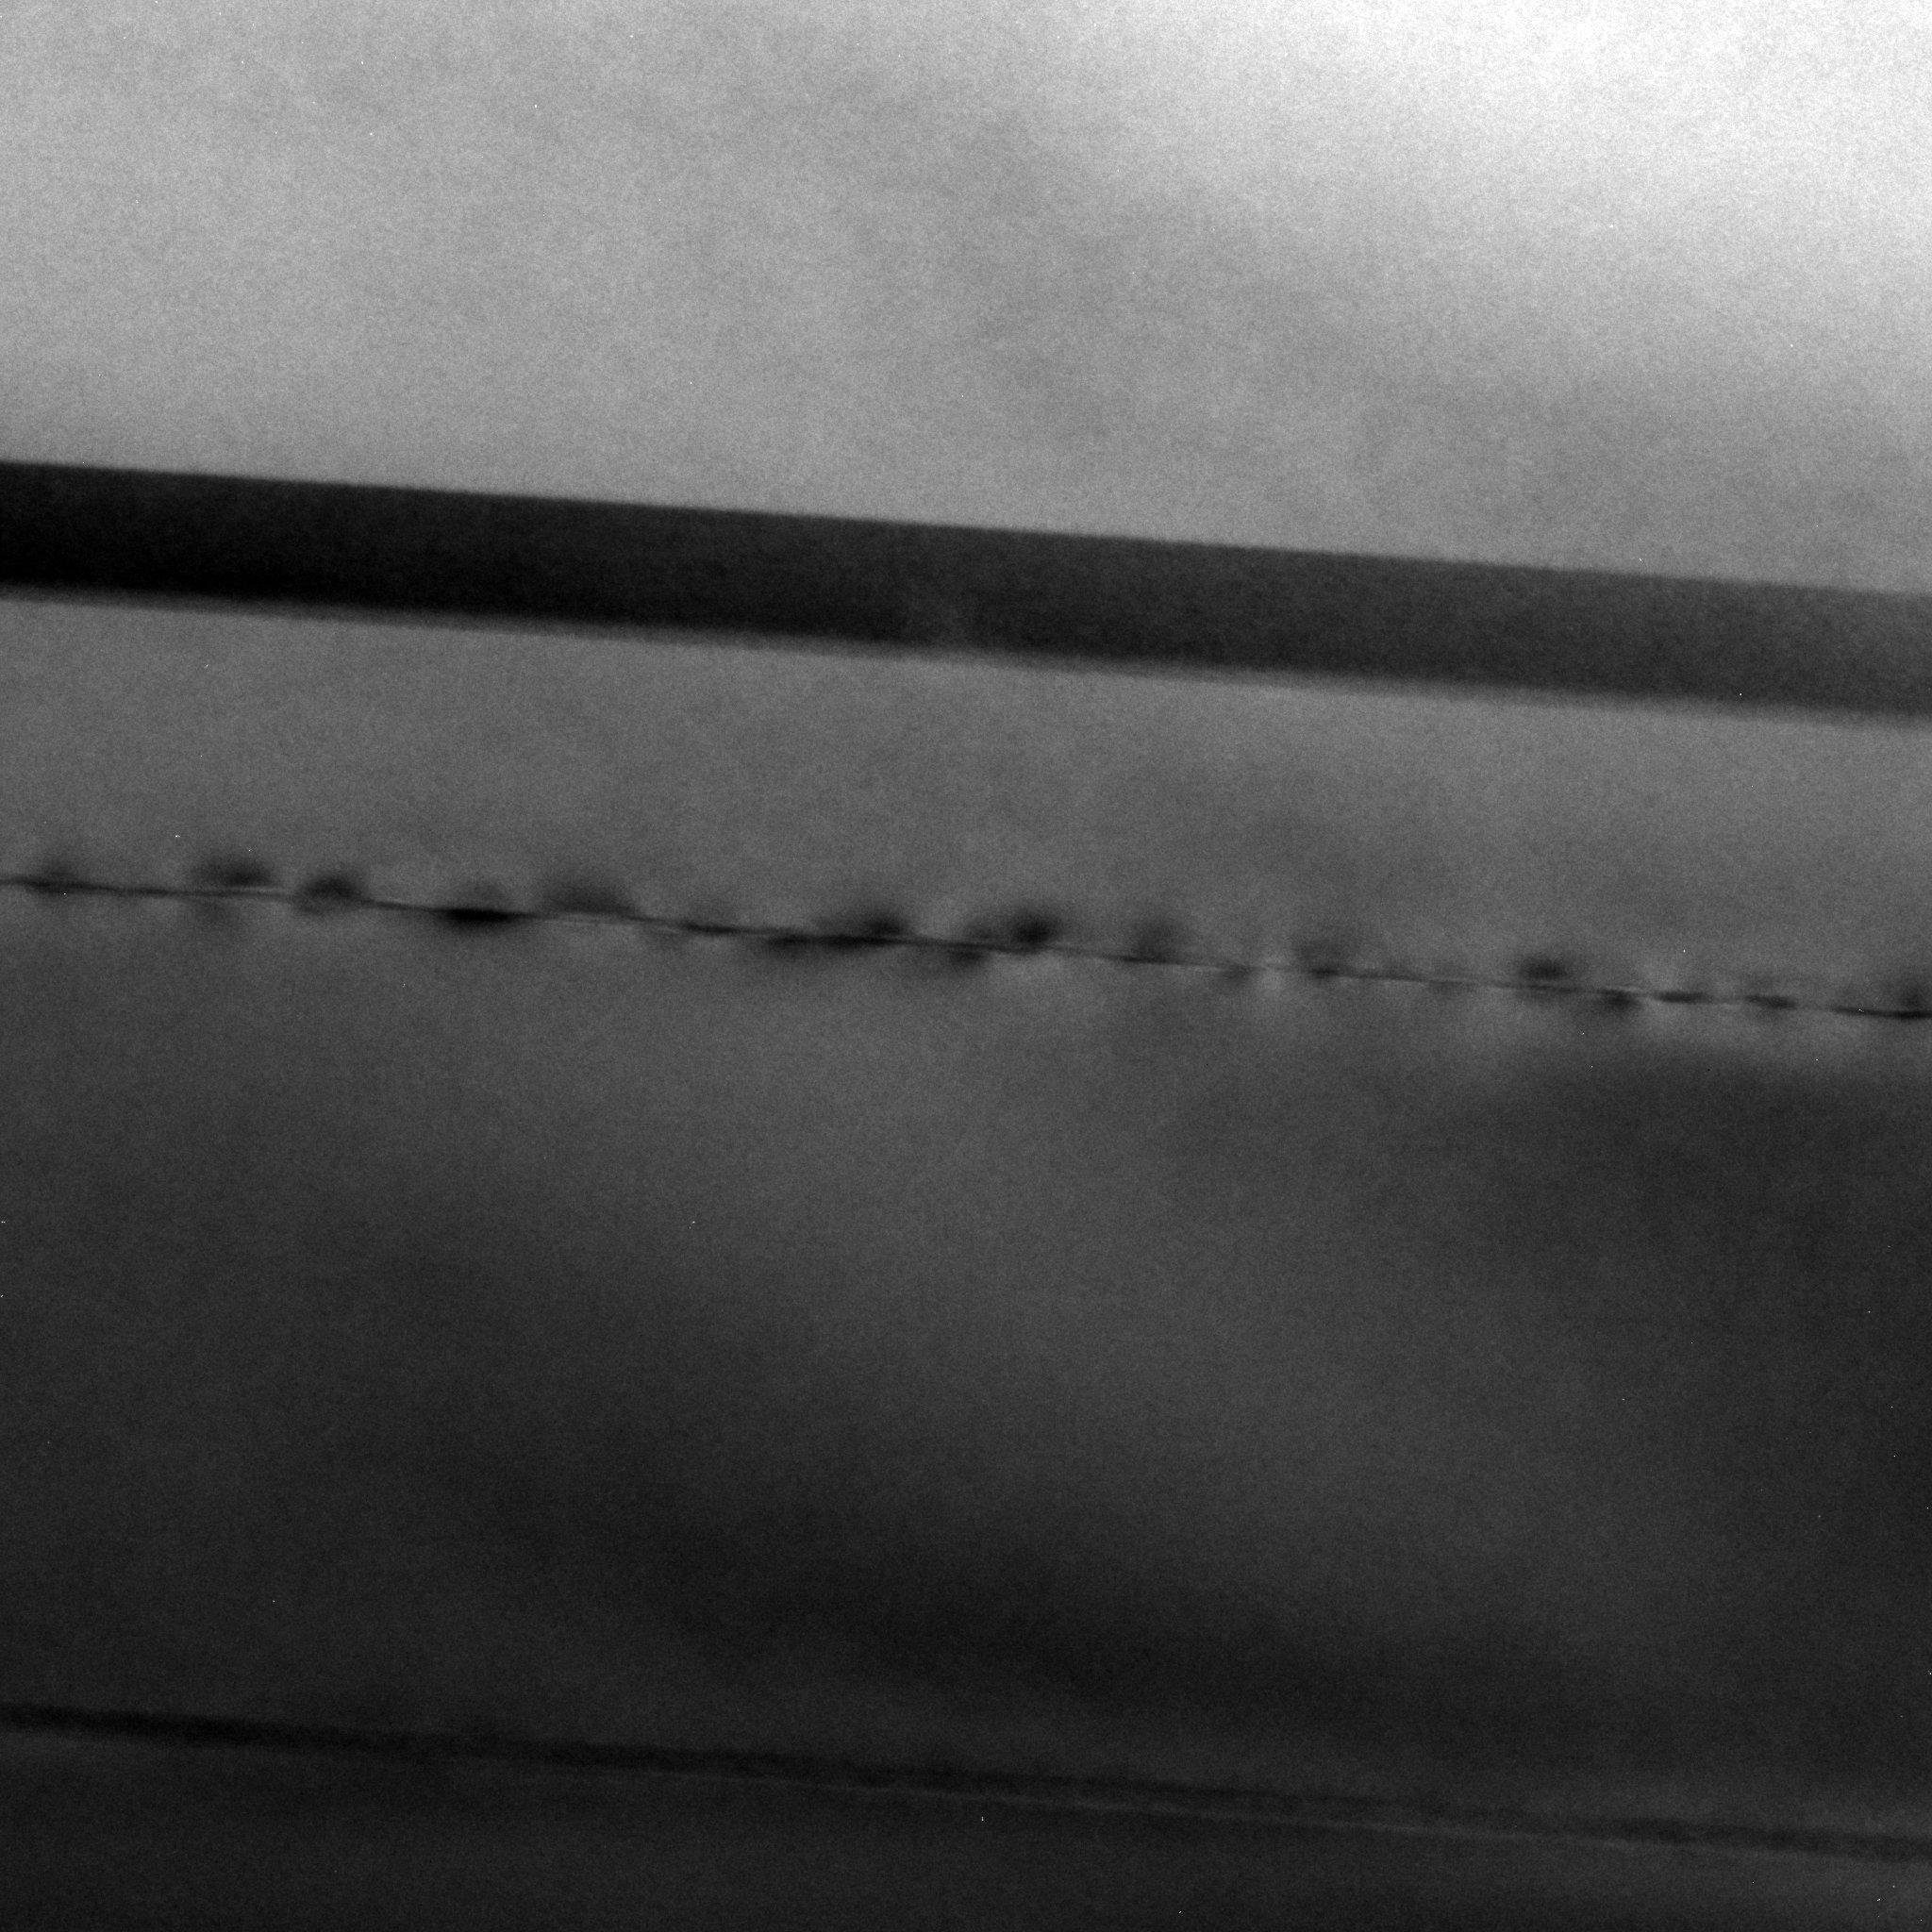
\includegraphics[width=\textwidth]{Grundlagen&Beugung/Eigeneprobe_BF_Al_Belt.jpg}
         \caption{Brightfield}
         \label{EPBFAl}
     \end{subfigure}
     \hfill
     \begin{subfigure}[b]{0.49\textwidth}
         \centering
         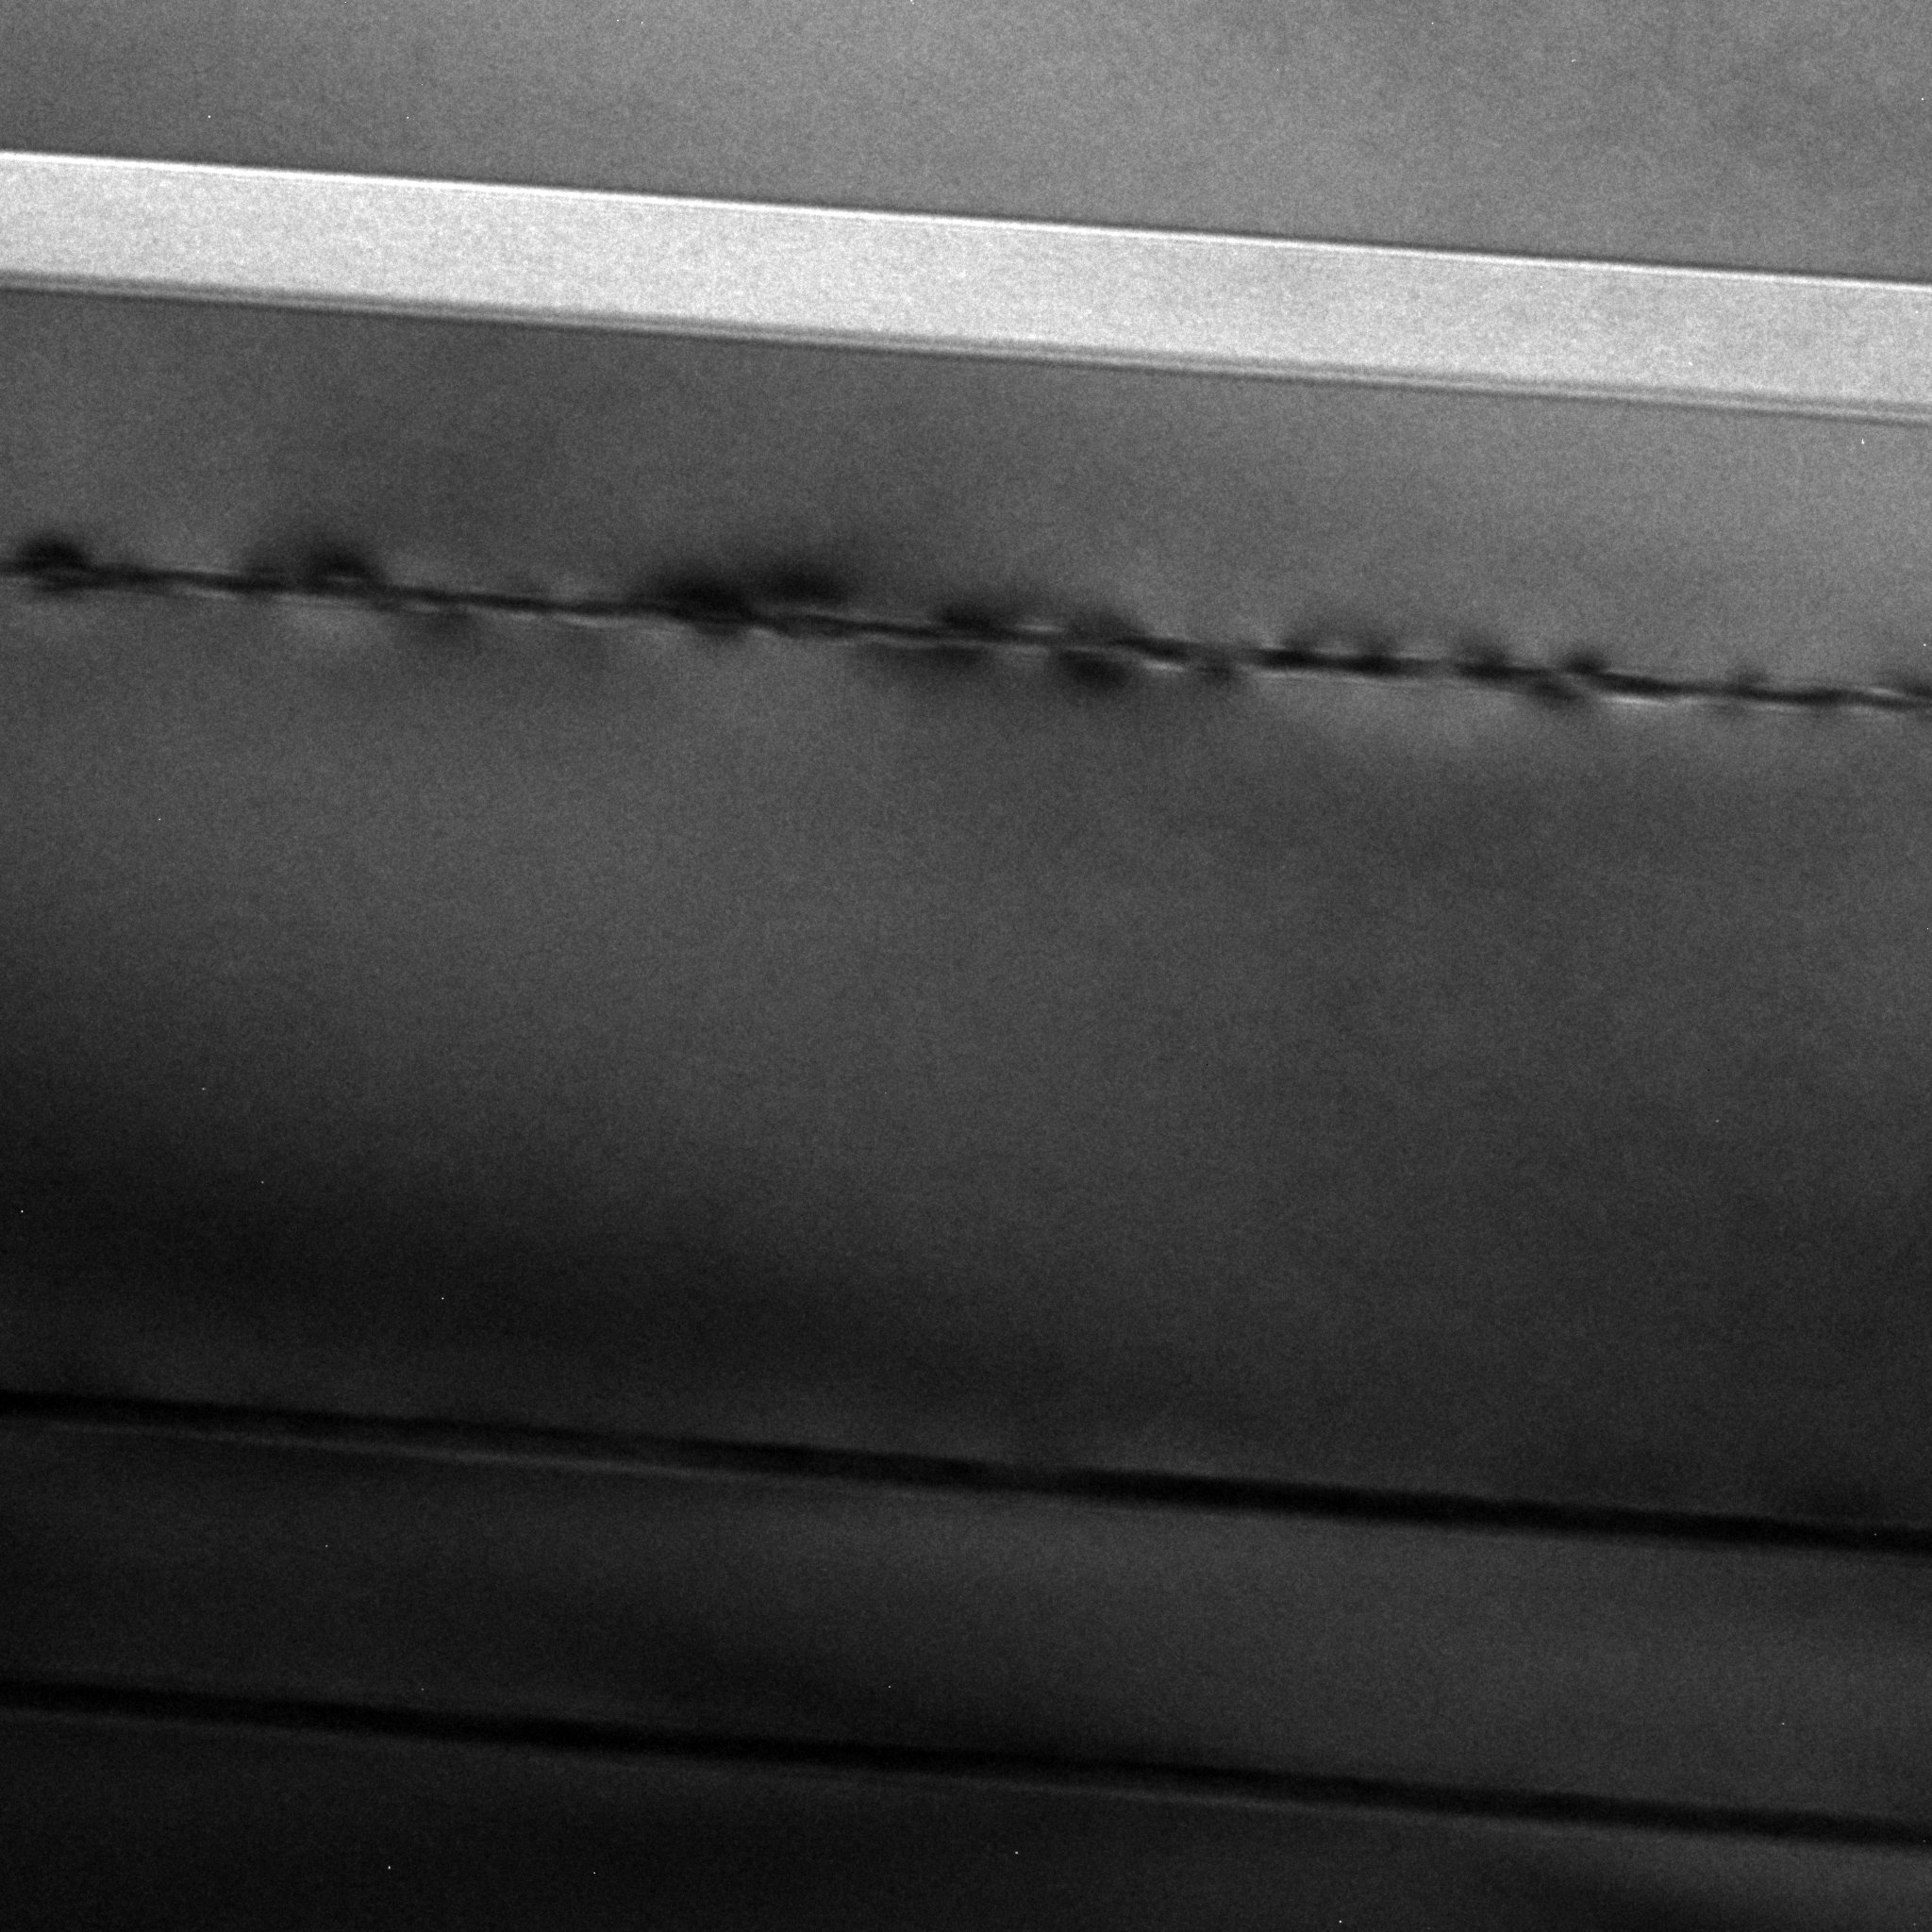
\includegraphics[width=\textwidth]{Grundlagen&Beugung/Eigeneprobe_DF_Al_Beld.jpg}
         \caption{Darkfield}
         \label{EPDFAl}
     \end{subfigure}
        \caption{TEM Darkfield und Brightfield Aufnahme GaAs Probe mit Al Belt.}
        \label{EPBF&DFAl}
\end{figure}

Die nächsten aufnahmen (Siehe \cref{EPBF&DFQB}) sind von den Quantum Belts, es wurden Jeweils Hell und Dunkel Feld aufnahmen. In der Dunkelfeld Aufnahme ist durch den hohen Kontrast die unterschiedliche dicke der Quantum Belts gut zu erkennen. 

\begin{figure}
     \centering
     \begin{subfigure}[b]{0.49\textwidth}
         \centering
         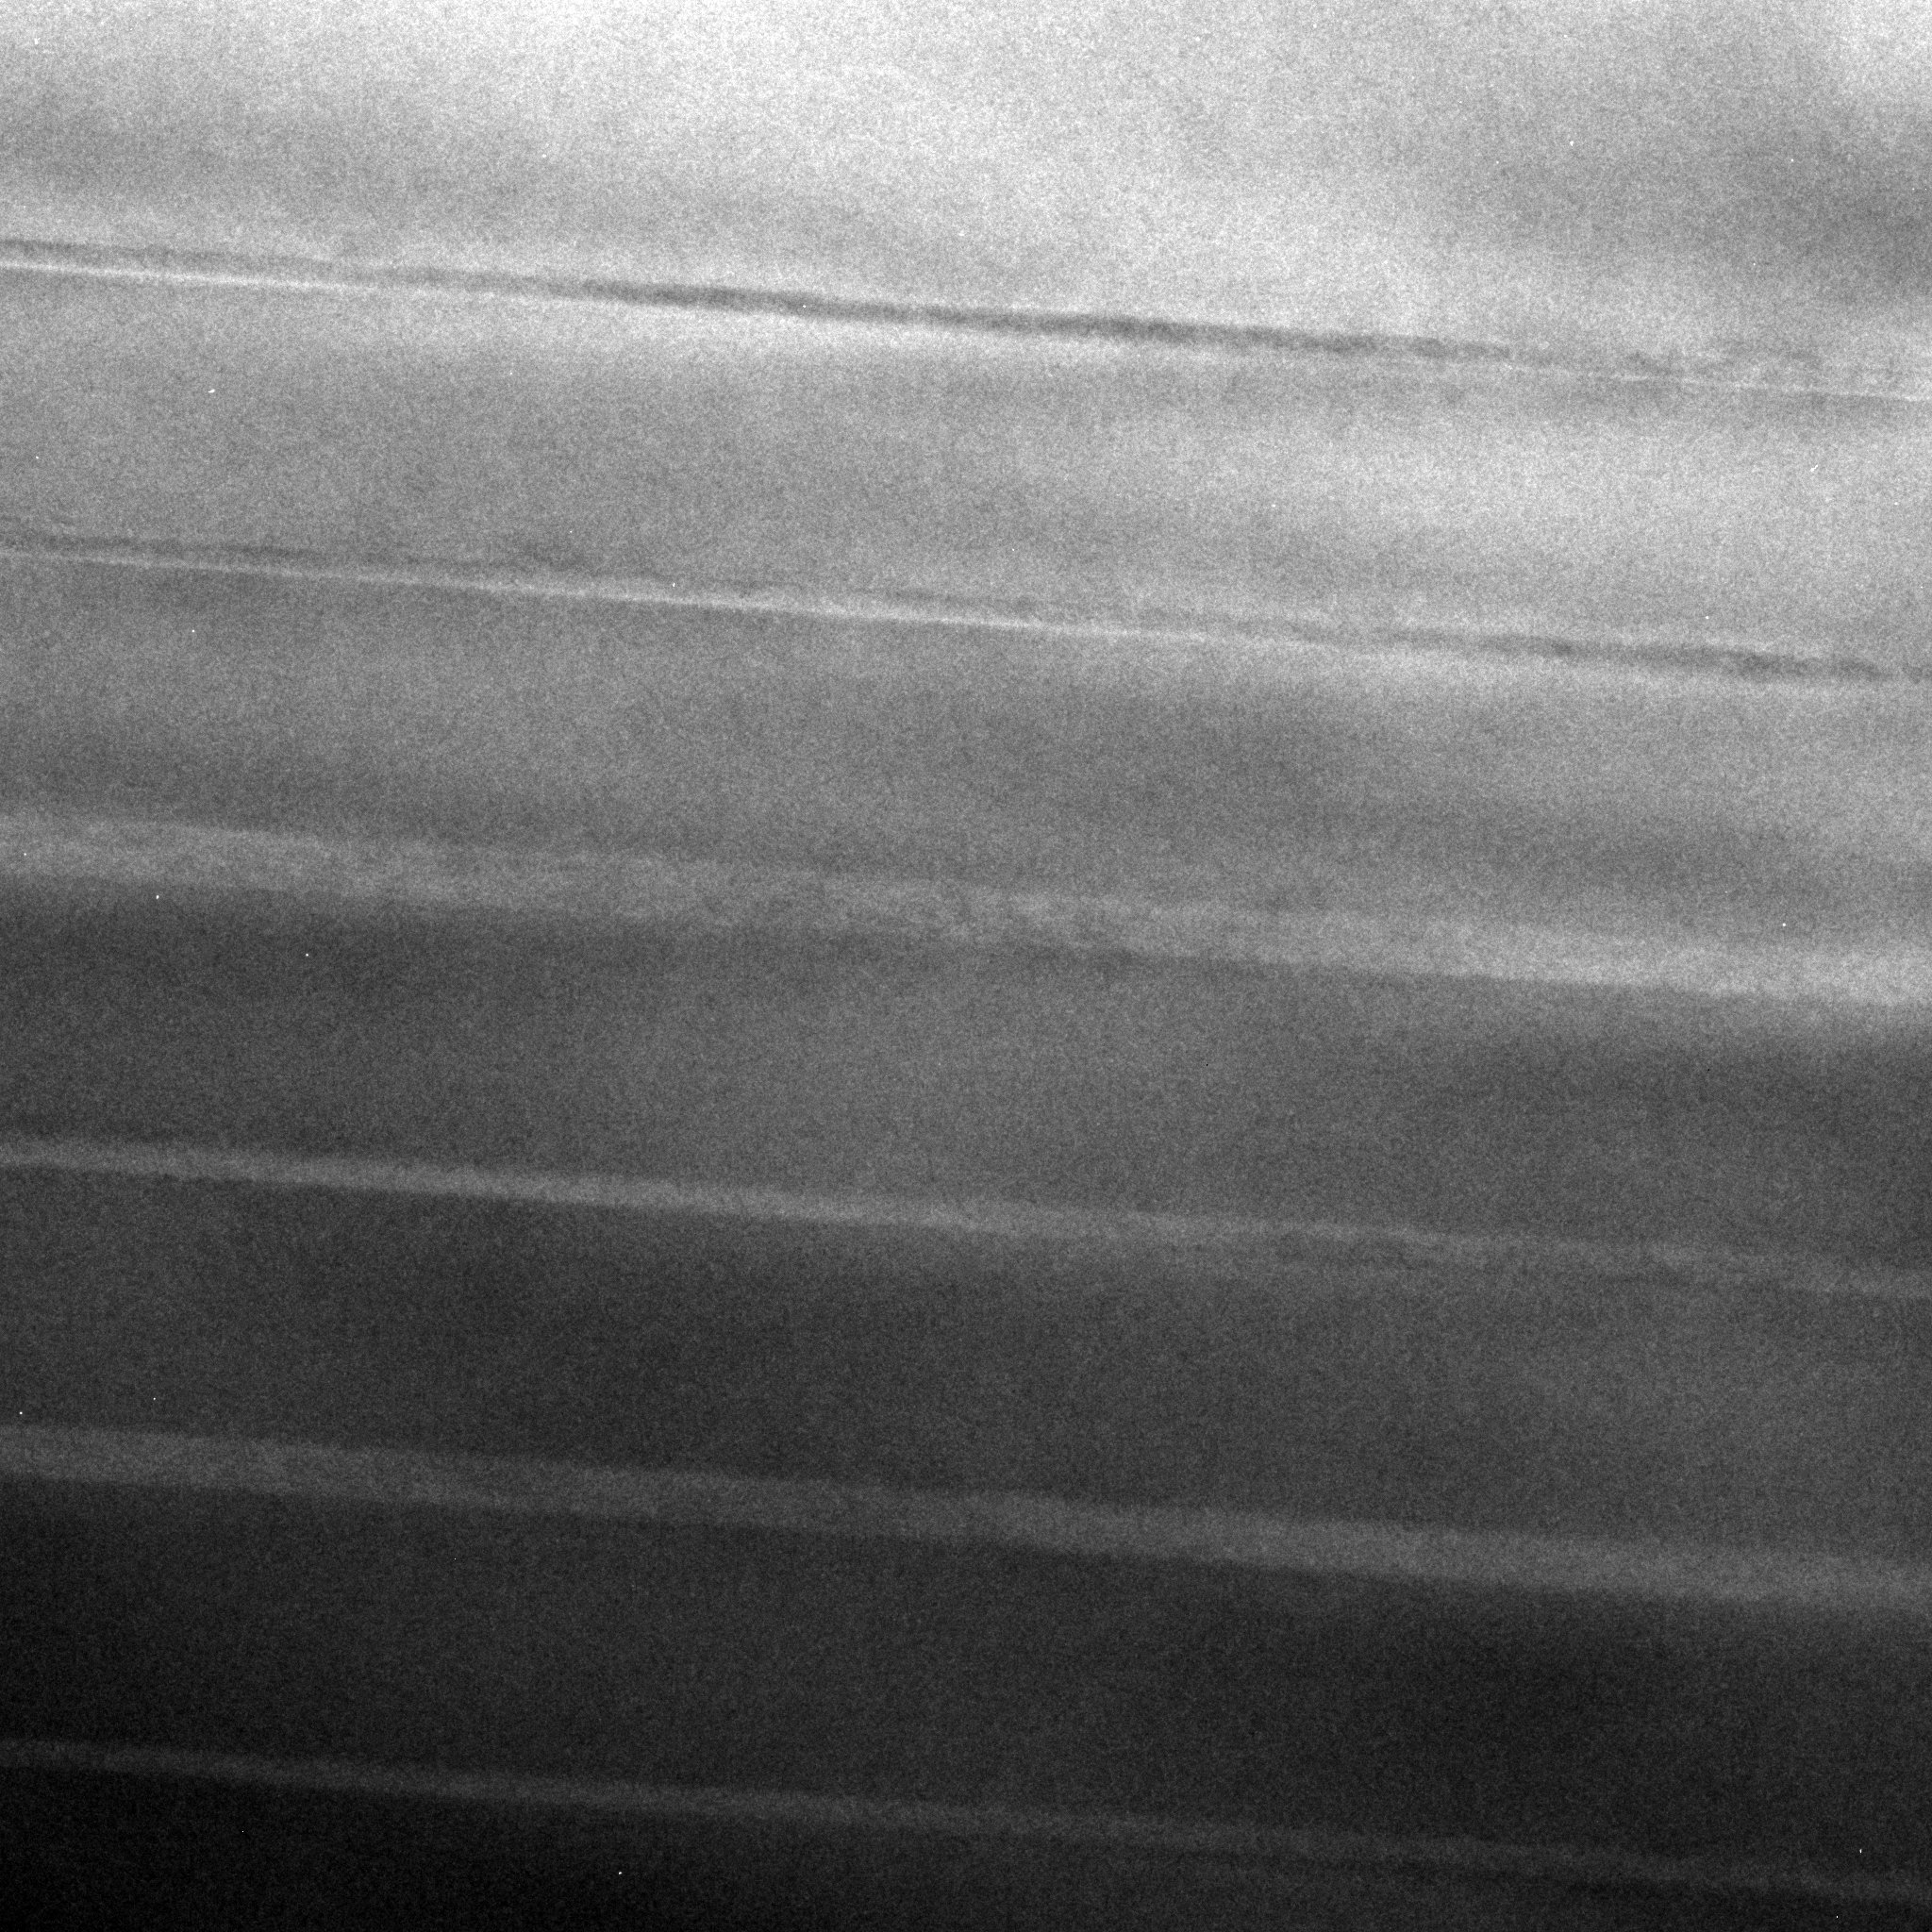
\includegraphics[width=\textwidth]{Grundlagen&Beugung/Eigeneprobe_BF_Quantumbelts_(true)2.jpg }
         \caption{Brightfield}
         \label{EPBFQB}
     \end{subfigure}
     \hfill
     \begin{subfigure}[b]{0.49\textwidth}
         \centering
         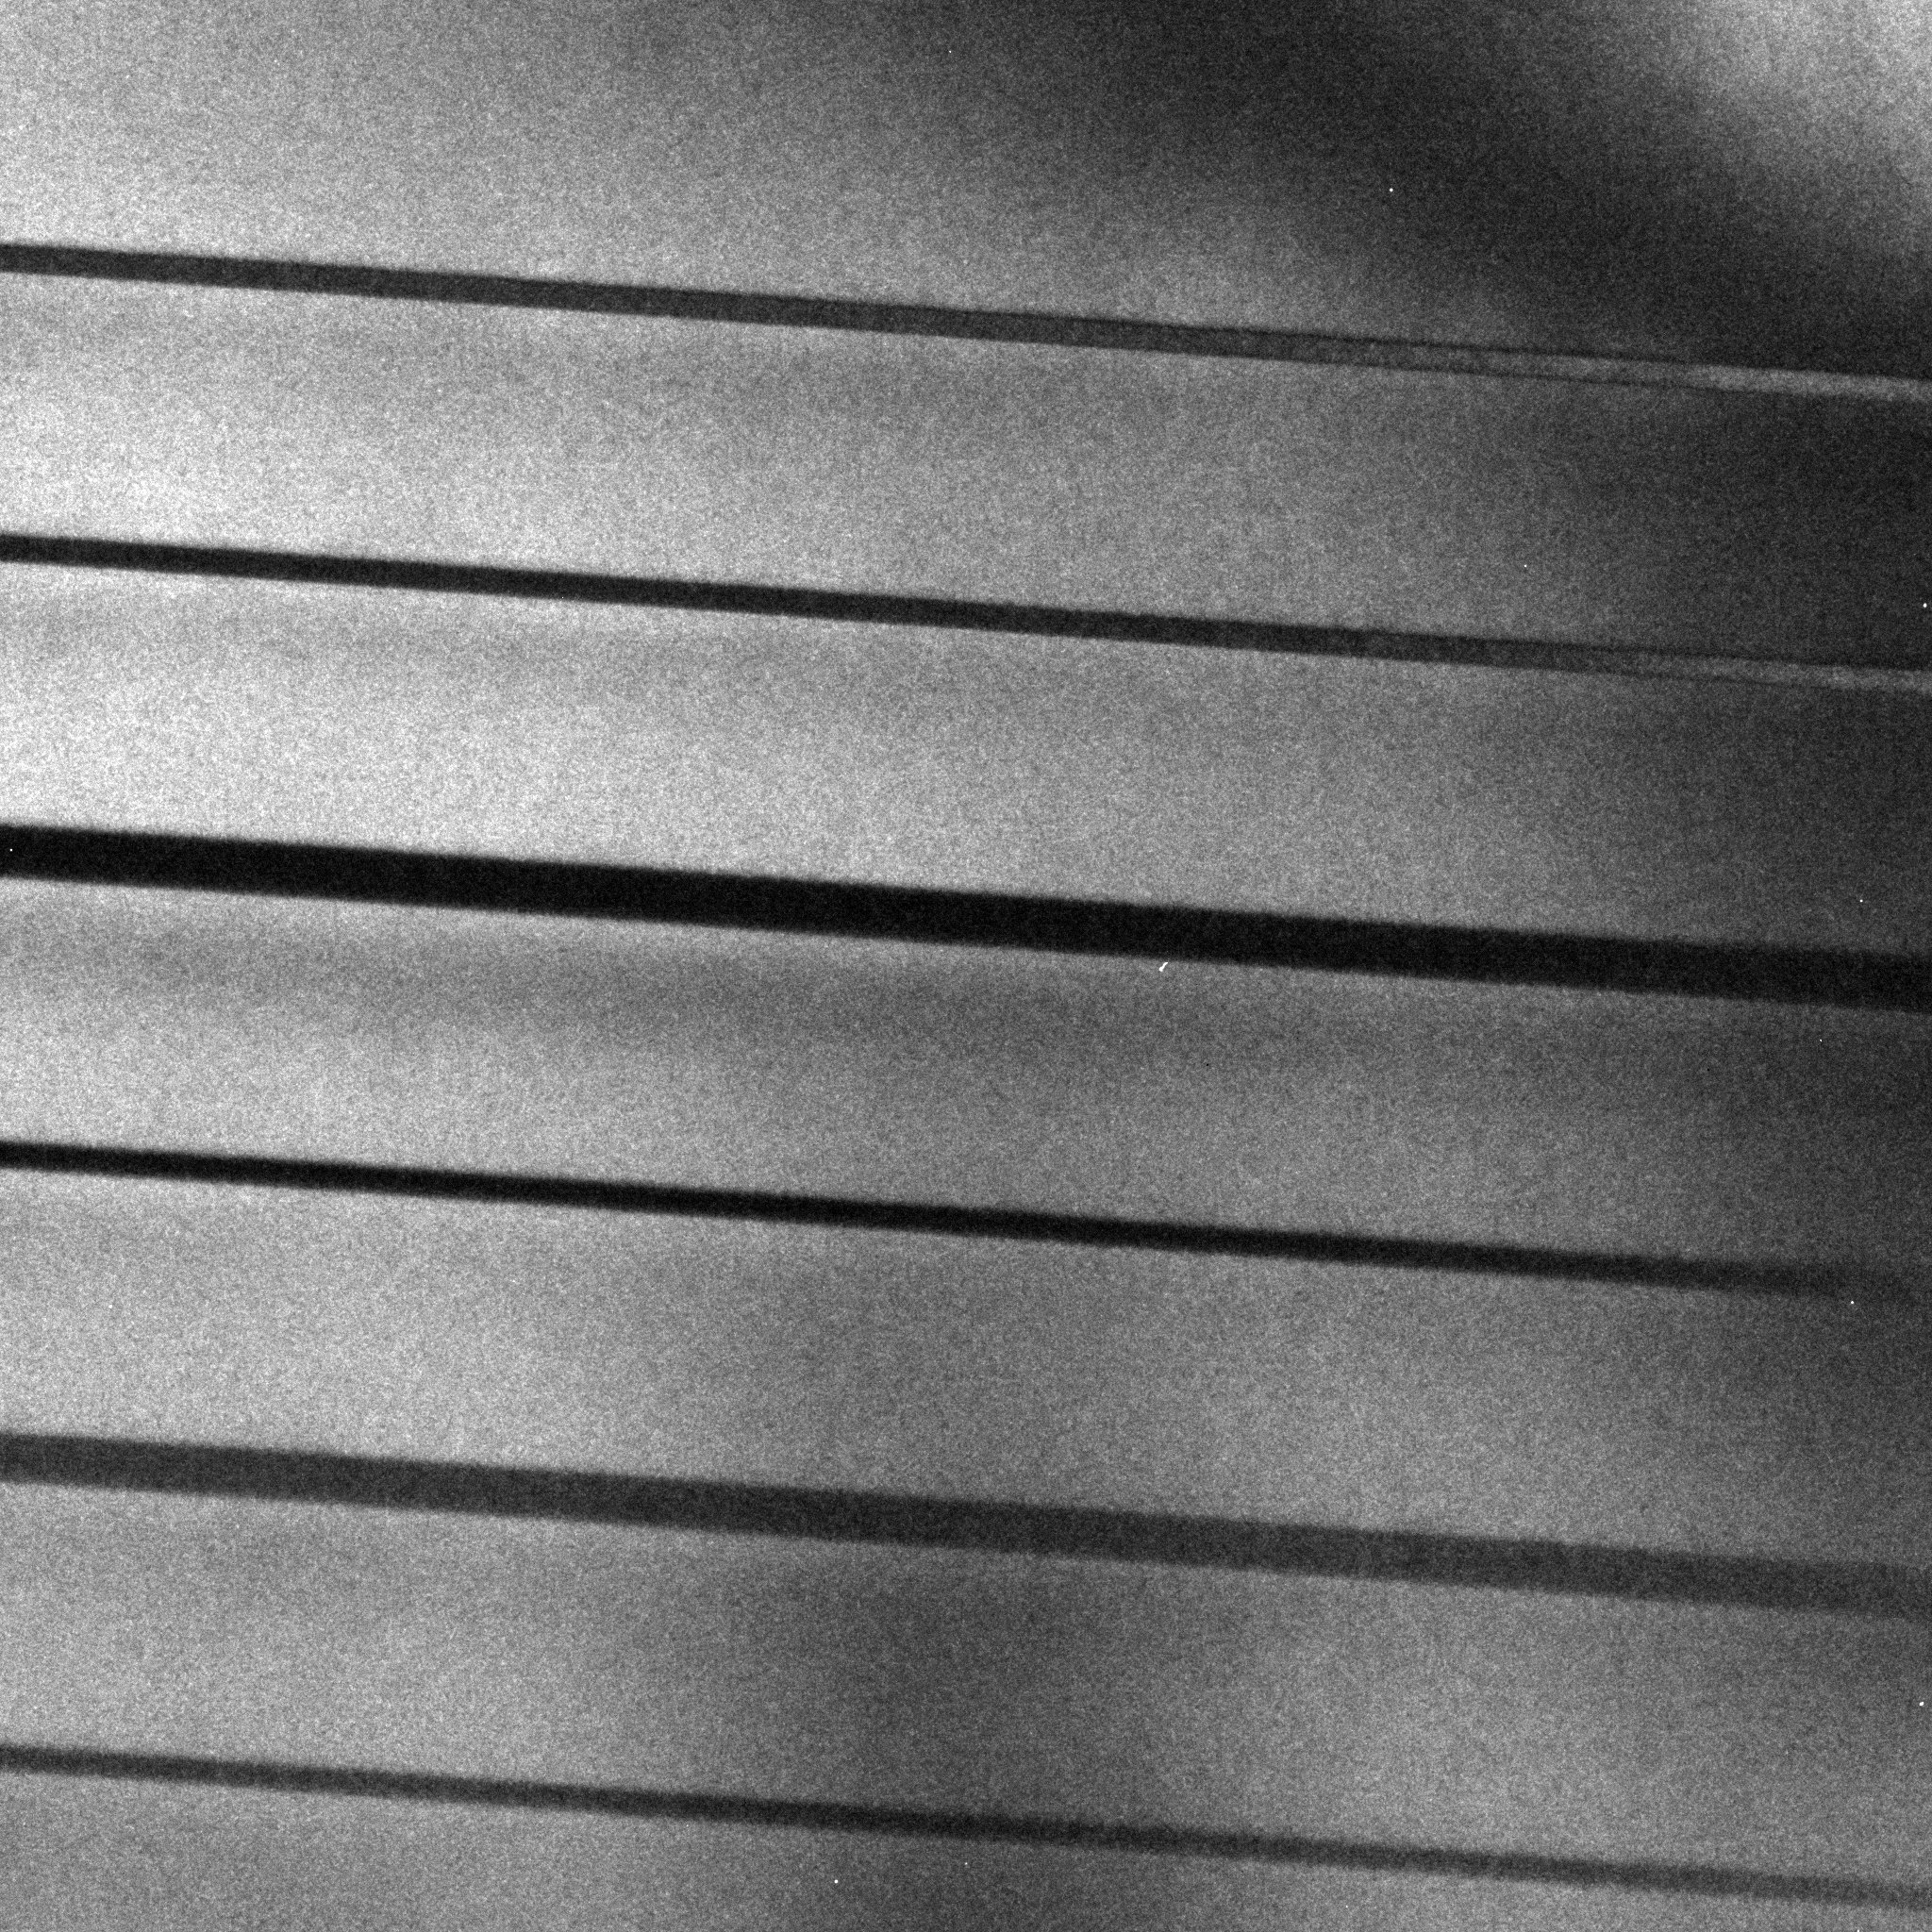
\includegraphics[width=\textwidth]{Grundlagen&Beugung/Eigeneprobe_DF_Quantumbelt_(true)2.jpg}
         \caption{Darkfield}
         \label{EPDFQB}
     \end{subfigure}
        \caption{TEM Darkfield und Brightfield Aufnahme GaAs Probe.}
        \label{EPBF&DFQB}
\end{figure}
